\chapter{\uppercase{Efficient and Safe Network Updates with Suffix Causal Consistency}}
\label{chap:scc}

In this chapter, we propose a new method to achieve efficient and safe network forwarding-state update using an alternative consistent update abstraction that we call \textit{suffix causal consistency}.
Unlike existing mechanisms~\cite{swan,dionysus,espres,zupdate,incrementalcu,timedcu}
which enforce atomicity, this approach allows packets to traverse a combination of
both old and new paths, thus relaxing the consistency model and speeding up update
times.  Our work builds on the following insights: (1) for most
network policies, the network paths are designed to control routes to
a destination (or a suffix), and (2) a packet (or a flow) traversing a
mixture of old and new paths can retain correctness provided it
traverses the old policy and then the new. These insights are a
natural fit for causal consistency~\cite{causal}, a shared memory
consistency model that guarantees that processes (in our case packets)
observe operations (in our case rules) in a causal order.  To this
end, we propose \textit{suffix causal consistency} (SCC), a practical and
efficient networking domain-specific realization of causal
consistency.

There are several challenges in practically realizing causal
consistency within the network of distributed devices.  The first is
designing update algorithms that provide causal consistency while
simultaneously preserving a broad range of network invariants,
e.g., black-hole freedom.  We tackle this challenge by tagging each
packet with a Lamport timestamp~\cite{LamportClock}; each switch then
updates this timestamp to reflect the rule matched to the packet.
Naively, this approach would then require that downstream switches
match this packet only to a rule with a timestamp at least as large,
but doing so requires that any network update affect \textit{all} of
these downstream switches (to increase their rule timestamps, even if
their rules need not change).  We thus propose a novel method of
managing these timestamps to limit the number of switches that each
network update must involve, thereby accelerating the update process.
A second challenge is developing network primitives to efficiently
support causal consistency on commodity switches in the face of
practical switch constraints and dynamic switch behavior. Despite the
development of highly programmable switches~\cite{P4Switch} that
unlock flexible functionality, support for causal consistency poses
several challenges. Specifically, supporting causal consistency
requires switches to detour packets and temporarily buffer
packets.

To demonstrate the effectiveness and efficiency of suffix causal
consistency, we developed prototypes for both Open vSwitch (OVS) and
P4~\cite{P4Switch}.  We evaluate our prototypes against realistic
workloads and topologies. Our analyses show that SCC deploys updates
faster than state-of-the-art alternatives (COCONUT~\cite{COCONUT}, TSU~\cite{tsu} and
CU~\cite{CU}) while simultaneously providing for less packet loss and
less rule overhead during updates.  We also show that our
rule-generation algorithm scales well to topologies of considerable
size.

Results of our evaluation show that:
\begin {enumerate*}
\item SCC outperforms COCONUT~\cite{COCONUT} and the original, uncoordinated approach to
rule updates in terms of the packets dropped during an update, and outperforms COCONUT,
CU~\cite{CU}, and TSU~\cite{tsu} in terms of the packets dropped due
to link failures.

\item SCC deploys rules more efficiently than CU, COCONUT, or
TSU and imposes less rule storage overhead in amount and/or duration than these alternatives.

\item The rule generation time of our algorithm scales across a range
of both fat-tree and ISP topologies.

\end {enumerate*}


\section{Network Model and Goals}
\label{sec:model}

In this section, we detail our model of the network, which is general
enough to include SDN setups and some others (\secref{sec:model:net}).
We then motivate and define our main goal in this dissertation, a property
that we call \textit{suffix causal consistency}
(\secref{sec:model:scc}).

\subsection{Network model}
\label{sec:model:net}

\paragraph{Controller}
The network has a logically centralized controller that is responsible
for configuring the switches.  To do so, the controller stores network
topology information, the \textit{rules} deployed on each switch
(i.e., flow table snapshot) as discussed below, and switch
configurations.  It makes network information available to one or more
\textit{applications} that make routing decisions.  The controller
produces a new routing policy as needed, based on input from
applications.  We refer to the emission of a new policy as a new
\textit{epoch}.  We assume that the routing policy of each new epoch
is deployed to the network (in the form of \textit{rules} described
below) before the next epoch begins.  Epochs are thus totally ordered
by time, and we use an epoch counter $\epochIdx = 1, 2, \ldots$ to
index a particular epoch.

\iffalse
An application informs the controller of a new route by calling the
interface \pathMod{\flowSpec}{\pathID{}}{\prtLevel} to specify a new
path \pathID{} (or drop action) for a set of flows specified by
\flowSpec (e.g., by IP 5-tuple).
\mkr{We don't use \prtLevel anywhere in the algorithm description or
  in the definition of SCC.  Suggest we drop this.}
The path \pathID{} is represented
by a list of switches $\switchID{\switchIdx} \rightarrow
... \rightarrow \switchID{\switchIdxAlt}$ where each $\switchID{}$ is
a switch id (or the application can specify $\dropAction$ to represent
the drop action). The priority level $\prtLevel$ indicates the
priority of this path.  \iffalse If the application requires higher
priority than other applications, it can issue commands with
$\prtLevel = high$ to ensure the rules deployed on switches of the
highest priority.  \fi The application leverages this interface to
provide a route change of a specific flow to the controller.  To
specify correctness for our protocol, we assume that the \pathMod
interface is invoked sequentially, and we denote by \pathModIdx the
index of a specific \pathMod invocation.
\fi

\paragraph{Routing policies} A routing policy specifies how to route
\textit{flows} through the network.  A flow consists of packets with
the same addressing information (IP 5-tuple).  We assume that the
packets of any flow enter the network at a single ingress point that
remains constant across epochs (as is commonly assumed,
e.g.,~\cite{CU}).
\iffalse
\footnote{This assumption can be relaxed through
  techniques to support migration, e.g.,~\cite{lime}.}
\fi

\paragraph{Rules}
The instructions for how a switch should treat certain packets are
specified by \textit{rules}.  Each rule \ruleID{} includes (at least)
the following fields, all of which are immutable:
\begin{itemize}
\item \ruleID{}{\coverField} specifies the set of flows to which
  this rule pertains (i.e., that can be matched to this rule);
\item \ruleID{}{\priorityField} specifies the priority of this rule,
  with higher priorities indicated by larger numbers and with a
  special priority $\infty$ to represent the maximum priority, which
  can be used only by our algorithm;
\item \ruleID{}{\sendToField} specifies the switch identifier (in
  practice, an outbound port) to which packets matched to this rule
  should be forwarded, or \dropAction if the packets should be
  dropped;
\item \ruleID{}{\switchField{}} specifies the unique switch
  \switchID{} into which \ruleID{} can be installed; and
\item \ruleID{}{\epochField{}} records the index \epochIdx of the
  epoch that produced this rule.
\end{itemize}

Each epoch yields a collection of rules for switches in the network to
implement the routing policy for this epoch.  That said, not all such
rules will necessarily be installed at (i.e., deployed to) switches,
since they may be redundant with rules already installed in some of
the switches.

\paragraph{Switches}
Each switch maintains a flow entry table which stores a set of rules
for flow management.  We denote the set of rules in the flow table of
switch \switchID{} as \switchID{}{\ruleSet}; e.g.,
$\switchID{}{\ruleSet} = \{\ruleID{1}, \ruleID{6}, \ruleID{10}\}$
means that switch \switchID{} includes rules $\ruleID{1}$,
$\ruleID{6}$ and $\ruleID{10}$.  The controller modifies this set by
invoking the following interface, which is similar to that provided by
OpenFlow:
\begin{itemize}
\item \switchID{}{\flowAdd{\ruleID{\ruleIdx}}} inserts rule
  \ruleID{\ruleIdx} into \switchID{}{\ruleSet}.  This command fails
  with no effect if $\ruleID{\ruleIdx}{\switchField} \neq \switchID{}$
  or if \switchID{}{\ruleSet} already contains a rule
  \ruleID{\ruleIdxAlt} such that $\ruleID{\ruleIdxAlt}{\priorityField}
  = \ruleID{\ruleIdx}{\priorityField}$ and
  $\ruleID{\ruleIdx}{\coverField} \cap
  \ruleID{\ruleIdxAlt}{\coverField} \neq \emptyset$.
\item \switchID{}{\flowDel{\ruleID{\ruleIdx}}} removes rule
  \ruleID{\ruleIdx} from \switchID{}{\ruleSet}.
\end{itemize}


Due to the communication delay between the controller and each switch,
invoking these switch commands on multiple switches simultaneously
cannot ensure that the switches reflect these changes at the same
time, which may cause inconsistent states across the switches. For
example, if one switch has already deleted a stale rule, but its
upstream switch still keeps sending packets to it, this switch may not
find a matching rule or leverage the default rule (which may drop the
packets and create a black hole).

\paragraph{An example}
Consider a packet \pktID{} that traverses a sequence of switches
$\switchID{\switchIdx} \rightarrow \ldots \rightarrow
\switchID{\switchIdxAlt}$, as directed by the rules on these switches,
written $\ruleID{\ruleIdx} \rightarrow \ldots \rightarrow
\ruleID{\ruleIdxAlt}$. For example, in \figref{fig:route}, the rules
applied to packet $\pktID{}$ on path $\switchID{1} \rightarrow
\switchID{2} \rightarrow \switchID{4} \rightarrow \switchID{5}$ are
$\ruleID{1} \rightarrow \ruleID{2} \rightarrow \ruleID{3} \rightarrow
\ruleID{4}$, where rule $\ruleID{1}$ directs switch $\switchID{1}$ to
send the packet $\pktID{}$ to switch $\switchID{2}$, and so on. If the
application wants to change the path of packet $\pktID{}$ from
$\switchID{1} \rightarrow \switchID{2} \rightarrow \switchID{4}
\rightarrow \switchID{5}$ (the dashed line in \figref{fig:route},
denoted \oldPath{\pktID{}}) to $\switchID{1} \rightarrow \switchID{3}
\rightarrow \switchID{4} \rightarrow \switchID{5}$ (the solid line,
denoted \newPath{\pktID{}}), then the application conveys this to the
controller, and the controller generates several commands to update
the switch states (resulting in a new epoch). The commands include:
\begin{itemize}
\item \switchID{1}{\flowDel{\ruleID{1}}} and
  \switchID{1}{\flowAdd{\ruleID{11}}}
  where\\ $\ruleID{11}{\sendToField} = \switchID{3}$ and $\pktID{}
  \in \ruleID{11}{\coverField}$;

\item \switchID{2}{\flowDel{\ruleID{2}}} to delete rule \ruleID{2}
  from \switchID{2}; and

\item \switchID{3}{\flowAdd{\ruleID{5}}} to instruct \switchID{3} to
  send \pktID{} to \switchID{4} (i.e., $\ruleID{5}{\sendToField} =
  \switchID{4}$ and $\pktID{} \in \ruleID{5}{\coverField}$).
\end{itemize}

Rule \ruleID{3} instructing \switchID{4} to send \pktID{} to
\switchID{5} need not be changed (assuming \ruleID{3}{\coverField}
does not specify the inbound port on \switchID{4}).  Nor does rule
\ruleID{4} instructing \switchID{5} to send \pktID{} to the
destination node.

\begin{figure}
\centering
\resizebox{0.75\linewidth}{!}{\small% Graphic for TeX using PGF
% Title: /Users/ziqiaozhou/GoogleDrive/sheng/svn/fig/example.dia
% Creator: Dia v0.97.2
% CreationDate: Tue Jan 30 21:33:30 2018
% For: ziqiaozhou
% \usepackage{tikz}
% The following commands are not supported in PSTricks at present
% We define them conditionally, so when they are implemented,
% this pgf file will use them.
\ifx\du\undefined
  \newlength{\du}
\fi
\setlength{\du}{4.8\unitlength}
\begin{tikzpicture}
\pgftransformxscale{1.000000}
\pgftransformyscale{-1.000000}
\definecolor{dialinecolor}{rgb}{0.000000, 0.000000, 0.000000}
\pgfsetstrokecolor{dialinecolor}
\definecolor{dialinecolor}{rgb}{1.000000, 1.000000, 1.000000}
\pgfsetfillcolor{dialinecolor}
\pgfsetlinewidth{0.100000\du}
\pgfsetdash{}{0pt}
\pgfsetdash{}{0pt}
\pgfsetbuttcap
\pgfsetmiterjoin
\pgfsetlinewidth{0.100000\du}
\pgfsetbuttcap
\pgfsetmiterjoin
\pgfsetdash{}{0pt}
\definecolor{dialinecolor}{rgb}{0.000000, 0.000000, 0.000000}
\pgfsetstrokecolor{dialinecolor}
\draw (62.600700\du,20.767400\du)--(62.600700\du,24.430619\du)--(66.996563\du,24.430619\du)--(66.996563\du,20.767400\du)--cycle;
\pgfsetlinewidth{0.010000\du}
\pgfsetbuttcap
\pgfsetmiterjoin
\pgfsetdash{}{0pt}
\definecolor{dialinecolor}{rgb}{0.000000, 0.000000, 0.000000}
\pgfsetstrokecolor{dialinecolor}
\draw (62.600700\du,20.767400\du)--(62.600700\du,24.430619\du)--(66.996563\du,24.430619\du)--(66.996563\du,20.767400\du)--cycle;
\pgfsetlinewidth{0.100000\du}
\pgfsetbuttcap
\pgfsetmiterjoin
\pgfsetdash{}{0pt}
\definecolor{dialinecolor}{rgb}{0.000000, 0.000000, 0.000000}
\pgfsetstrokecolor{dialinecolor}
\draw (62.844915\du,21.011615\du)--(62.844915\du,23.942190\du)--(66.752348\du,23.942190\du)--(66.752348\du,21.011615\du)--cycle;
\pgfsetlinewidth{0.010000\du}
\pgfsetbuttcap
\pgfsetmiterjoin
\pgfsetdash{}{0pt}
\definecolor{dialinecolor}{rgb}{0.000000, 0.000000, 0.000000}
\pgfsetstrokecolor{dialinecolor}
\draw (62.844915\du,21.011615\du)--(62.844915\du,23.942190\du)--(66.752348\du,23.942190\du)--(66.752348\du,21.011615\du)--cycle;
\pgfsetlinewidth{0.100000\du}
\pgfsetbuttcap
\pgfsetmiterjoin
\pgfsetdash{}{0pt}
\definecolor{dialinecolor}{rgb}{0.000000, 0.000000, 0.000000}
\pgfsetstrokecolor{dialinecolor}
\draw (63.333344\du,24.430619\du)--(66.263919\du,24.430619\du)--(65.531275\du,24.674834\du)--(64.065988\du,24.674834\du)--cycle;
\pgfsetlinewidth{0.010000\du}
\pgfsetbuttcap
\pgfsetmiterjoin
\pgfsetdash{}{0pt}
\definecolor{dialinecolor}{rgb}{0.000000, 0.000000, 0.000000}
\pgfsetstrokecolor{dialinecolor}
\draw (63.333344\du,24.430619\du)--(66.263919\du,24.430619\du)--(65.531275\du,24.674834\du)--(64.065988\du,24.674834\du)--cycle;
\pgfsetlinewidth{0.100000\du}
\pgfsetbuttcap
\pgfsetmiterjoin
\pgfsetdash{}{0pt}
\definecolor{dialinecolor}{rgb}{0.000000, 0.000000, 0.000000}
\pgfsetstrokecolor{dialinecolor}
\draw (64.065988\du,24.674834\du)--(64.065988\du,24.919048\du)--(65.531275\du,24.919048\du)--(65.531275\du,24.674834\du)--cycle;
\pgfsetlinewidth{0.010000\du}
\pgfsetbuttcap
\pgfsetmiterjoin
\pgfsetdash{}{0pt}
\definecolor{dialinecolor}{rgb}{0.000000, 0.000000, 0.000000}
\pgfsetstrokecolor{dialinecolor}
\draw (64.065988\du,24.674834\du)--(64.065988\du,24.919048\du)--(65.531275\du,24.919048\du)--(65.531275\du,24.674834\du)--cycle;
\pgfsetlinewidth{0.100000\du}
\pgfsetbuttcap
\pgfsetmiterjoin
\pgfsetdash{}{0pt}
\definecolor{dialinecolor}{rgb}{0.000000, 0.000000, 0.000000}
\pgfsetstrokecolor{dialinecolor}
\draw (63.333344\du,24.919048\du)--(63.333344\du,25.163263\du)--(66.263919\du,25.163263\du)--(66.263919\du,24.919048\du)--cycle;
\pgfsetlinewidth{0.010000\du}
\pgfsetbuttcap
\pgfsetmiterjoin
\pgfsetdash{}{0pt}
\definecolor{dialinecolor}{rgb}{0.000000, 0.000000, 0.000000}
\pgfsetstrokecolor{dialinecolor}
\draw (63.333344\du,24.919048\du)--(63.333344\du,25.163263\du)--(66.263919\du,25.163263\du)--(66.263919\du,24.919048\du)--cycle;
\pgfsetlinewidth{0.100000\du}
\pgfsetdash{}{0pt}
\pgfsetdash{}{0pt}
\pgfsetbuttcap
\pgfsetmiterjoin
\pgfsetlinewidth{0.100000\du}
\pgfsetbuttcap
\pgfsetmiterjoin
\pgfsetdash{}{0pt}
\definecolor{dialinecolor}{rgb}{0.000000, 0.000000, 0.000000}
\pgfsetstrokecolor{dialinecolor}
\draw (11.599100\du,20.671200\du)--(11.599100\du,24.334419\du)--(15.994963\du,24.334419\du)--(15.994963\du,20.671200\du)--cycle;
\pgfsetlinewidth{0.010000\du}
\pgfsetbuttcap
\pgfsetmiterjoin
\pgfsetdash{}{0pt}
\definecolor{dialinecolor}{rgb}{0.000000, 0.000000, 0.000000}
\pgfsetstrokecolor{dialinecolor}
\draw (11.599100\du,20.671200\du)--(11.599100\du,24.334419\du)--(15.994963\du,24.334419\du)--(15.994963\du,20.671200\du)--cycle;
\pgfsetlinewidth{0.100000\du}
\pgfsetbuttcap
\pgfsetmiterjoin
\pgfsetdash{}{0pt}
\definecolor{dialinecolor}{rgb}{0.000000, 0.000000, 0.000000}
\pgfsetstrokecolor{dialinecolor}
\draw (11.843315\du,20.915415\du)--(11.843315\du,23.845990\du)--(15.750748\du,23.845990\du)--(15.750748\du,20.915415\du)--cycle;
\pgfsetlinewidth{0.010000\du}
\pgfsetbuttcap
\pgfsetmiterjoin
\pgfsetdash{}{0pt}
\definecolor{dialinecolor}{rgb}{0.000000, 0.000000, 0.000000}
\pgfsetstrokecolor{dialinecolor}
\draw (11.843315\du,20.915415\du)--(11.843315\du,23.845990\du)--(15.750748\du,23.845990\du)--(15.750748\du,20.915415\du)--cycle;
\pgfsetlinewidth{0.100000\du}
\pgfsetbuttcap
\pgfsetmiterjoin
\pgfsetdash{}{0pt}
\definecolor{dialinecolor}{rgb}{0.000000, 0.000000, 0.000000}
\pgfsetstrokecolor{dialinecolor}
\draw (12.331744\du,24.334419\du)--(15.262319\du,24.334419\du)--(14.529675\du,24.578634\du)--(13.064388\du,24.578634\du)--cycle;
\pgfsetlinewidth{0.010000\du}
\pgfsetbuttcap
\pgfsetmiterjoin
\pgfsetdash{}{0pt}
\definecolor{dialinecolor}{rgb}{0.000000, 0.000000, 0.000000}
\pgfsetstrokecolor{dialinecolor}
\draw (12.331744\du,24.334419\du)--(15.262319\du,24.334419\du)--(14.529675\du,24.578634\du)--(13.064388\du,24.578634\du)--cycle;
\pgfsetlinewidth{0.100000\du}
\pgfsetbuttcap
\pgfsetmiterjoin
\pgfsetdash{}{0pt}
\definecolor{dialinecolor}{rgb}{0.000000, 0.000000, 0.000000}
\pgfsetstrokecolor{dialinecolor}
\draw (13.064388\du,24.578634\du)--(13.064388\du,24.822848\du)--(14.529675\du,24.822848\du)--(14.529675\du,24.578634\du)--cycle;
\pgfsetlinewidth{0.010000\du}
\pgfsetbuttcap
\pgfsetmiterjoin
\pgfsetdash{}{0pt}
\definecolor{dialinecolor}{rgb}{0.000000, 0.000000, 0.000000}
\pgfsetstrokecolor{dialinecolor}
\draw (13.064388\du,24.578634\du)--(13.064388\du,24.822848\du)--(14.529675\du,24.822848\du)--(14.529675\du,24.578634\du)--cycle;
\pgfsetlinewidth{0.100000\du}
\pgfsetbuttcap
\pgfsetmiterjoin
\pgfsetdash{}{0pt}
\definecolor{dialinecolor}{rgb}{0.000000, 0.000000, 0.000000}
\pgfsetstrokecolor{dialinecolor}
\draw (12.331744\du,24.822848\du)--(12.331744\du,25.067063\du)--(15.262319\du,25.067063\du)--(15.262319\du,24.822848\du)--cycle;
\pgfsetlinewidth{0.010000\du}
\pgfsetbuttcap
\pgfsetmiterjoin
\pgfsetdash{}{0pt}
\definecolor{dialinecolor}{rgb}{0.000000, 0.000000, 0.000000}
\pgfsetstrokecolor{dialinecolor}
\draw (12.331744\du,24.822848\du)--(12.331744\du,25.067063\du)--(15.262319\du,25.067063\du)--(15.262319\du,24.822848\du)--cycle;
\pgfsetlinewidth{0.350000\du}
\pgfsetdash{}{0pt}
\pgfsetdash{}{0pt}
\definecolor{dialinecolor}{rgb}{0.000000, 0.000000, 0.000000}
\pgfsetstrokecolor{dialinecolor}
\pgfpathellipse{\pgfpoint{23.108200\du}{22.875300\du}}{\pgfpoint{2.725000\du}{0\du}}{\pgfpoint{0\du}{2.775000\du}}
\pgfusepath{stroke}
% setfont left to latex
\definecolor{dialinecolor}{rgb}{0.000000, 0.000000, 0.000000}
\pgfsetstrokecolor{dialinecolor}
\node[anchor=west] at (20.542400\du,23.134800\du){\switchID{1}};
\pgfsetlinewidth{0.350000\du}
\pgfsetdash{}{0pt}
\pgfsetdash{}{0pt}
\definecolor{dialinecolor}{rgb}{0.000000, 0.000000, 0.000000}
\pgfsetstrokecolor{dialinecolor}
\pgfpathellipse{\pgfpoint{43.559900\du}{22.966400\du}}{\pgfpoint{2.725000\du}{0\du}}{\pgfpoint{0\du}{2.775000\du}}
\pgfusepath{stroke}
% setfont left to latex
\definecolor{dialinecolor}{rgb}{0.000000, 0.000000, 0.000000}
\pgfsetstrokecolor{dialinecolor}
\node[anchor=west] at (41.067400\du,23.275000\du){\switchID{4}};
% setfont left to latex
\definecolor{dialinecolor}{rgb}{0.000000, 0.000000, 0.000000}
\pgfsetstrokecolor{dialinecolor}
\node at (13.901300\du,22.437500\du){Src};
% setfont left to latex
\definecolor{dialinecolor}{rgb}{0.000000, 0.000000, 0.000000}
\pgfsetstrokecolor{dialinecolor}
\node at (64.920700\du,22.702400\du){Dst};
\pgfsetlinewidth{0.350000\du}
\pgfsetdash{}{0pt}
\pgfsetdash{}{0pt}
\pgfsetbuttcap
{
\definecolor{dialinecolor}{rgb}{0.000000, 0.000000, 0.000000}
\pgfsetfillcolor{dialinecolor}
% was here!!!
\pgfsetarrowsend{stealth}
\definecolor{dialinecolor}{rgb}{0.000000, 0.000000, 0.000000}
\pgfsetstrokecolor{dialinecolor}
\draw (16.295000\du,22.869524\du)--(20.083200\du,22.874876\du);
}
\pgfsetlinewidth{0.350000\du}
\pgfsetdash{{1.000000\du}{1.000000\du}}{0\du}
\pgfsetdash{{0.300000\du}{0.300000\du}}{0\du}
\pgfsetbuttcap
{
\definecolor{dialinecolor}{rgb}{0.000000, 0.000000, 0.000000}
\pgfsetfillcolor{dialinecolor}
% was here!!!
\pgfsetarrowsend{stealth}
\definecolor{dialinecolor}{rgb}{0.000000, 0.000000, 0.000000}
\pgfsetstrokecolor{dialinecolor}
\draw (25.673735\du,20.934066\du)--(30.321867\du,17.417018\du);
}
\pgfsetlinewidth{0.350000\du}
\pgfsetdash{{0.300000\du}{0.300000\du}}{0\du}
\pgfsetdash{{0.300000\du}{0.300000\du}}{0\du}
\pgfsetbuttcap
{
\definecolor{dialinecolor}{rgb}{0.000000, 0.000000, 0.000000}
\pgfsetfillcolor{dialinecolor}
% was here!!!
\pgfsetarrowsend{stealth}
\definecolor{dialinecolor}{rgb}{0.000000, 0.000000, 0.000000}
\pgfsetstrokecolor{dialinecolor}
\draw (35.126616\du,17.107073\du)--(40.921284\du,21.133127\du);
}
\pgfsetlinewidth{0.350000\du}
\pgfsetdash{}{0pt}
\pgfsetdash{}{0pt}
\pgfsetbuttcap
{
\definecolor{dialinecolor}{rgb}{0.000000, 0.000000, 0.000000}
\pgfsetfillcolor{dialinecolor}
% was here!!!
\pgfsetarrowsend{stealth}
\definecolor{dialinecolor}{rgb}{0.000000, 0.000000, 0.000000}
\pgfsetstrokecolor{dialinecolor}
\draw (25.796453\du,24.638739\du)--(30.173147\du,27.509761\du);
}
\pgfsetlinewidth{0.350000\du}
\pgfsetdash{}{0pt}
\pgfsetdash{}{0pt}
\pgfsetbuttcap
{
\definecolor{dialinecolor}{rgb}{0.000000, 0.000000, 0.000000}
\pgfsetfillcolor{dialinecolor}
% was here!!!
\pgfsetarrowsend{stealth}
\definecolor{dialinecolor}{rgb}{0.000000, 0.000000, 0.000000}
\pgfsetstrokecolor{dialinecolor}
\draw (46.584898\du,22.965235\du)--(51.097305\du,22.947717\du);
}
% setfont left to latex
\definecolor{dialinecolor}{rgb}{0.000000, 0.000000, 0.000000}
\pgfsetstrokecolor{dialinecolor}
\node[anchor=west] at (35.058200\du,14.140300\du){};
% setfont left to latex
\definecolor{dialinecolor}{rgb}{0.000000, 0.000000, 0.000000}
\pgfsetstrokecolor{dialinecolor}
\node[anchor=west] at (17.158200\du,7.840290\du){};
% setfont left to latex
\definecolor{dialinecolor}{rgb}{0.000000, 0.000000, 0.000000}
\pgfsetstrokecolor{dialinecolor}
\node[anchor=west] at (17.903200\du,7.840290\du){};
% setfont left to latex
\definecolor{dialinecolor}{rgb}{0.000000, 0.000000, 0.000000}
\pgfsetstrokecolor{dialinecolor}
\node[anchor=west] at (24.221200\du,28.042700\du){};
% setfont left to latex
\definecolor{dialinecolor}{rgb}{0.000000, 0.000000, 0.000000}
\pgfsetstrokecolor{dialinecolor}
\node[anchor=west] at (32.908200\du,24.290300\du){};
\pgfsetlinewidth{0.350000\du}
\pgfsetdash{}{0pt}
\pgfsetdash{}{0pt}
\pgfsetbuttcap
{
\definecolor{dialinecolor}{rgb}{0.000000, 0.000000, 0.000000}
\pgfsetfillcolor{dialinecolor}
% was here!!!
\pgfsetarrowsend{stealth}
\definecolor{dialinecolor}{rgb}{0.000000, 0.000000, 0.000000}
\pgfsetstrokecolor{dialinecolor}
\draw (35.057133\du,27.177749\du)--(40.683519\du,24.391048\du);
}
% setfont left to latex
\definecolor{dialinecolor}{rgb}{0.000000, 0.000000, 0.000000}
\pgfsetstrokecolor{dialinecolor}
\node[anchor=west] at (20.908200\du,26.865300\du){};
% setfont left to latex
\definecolor{dialinecolor}{rgb}{0.000000, 0.000000, 0.000000}
\pgfsetstrokecolor{dialinecolor}
\node[anchor=west] at (32.658200\du,24.465300\du){};
% setfont left to latex
\definecolor{dialinecolor}{rgb}{0.000000, 0.000000, 0.000000}
\pgfsetstrokecolor{dialinecolor}
\node[anchor=west] at (46.758200\du,24.915300\du){};
% setfont left to latex
\definecolor{dialinecolor}{rgb}{0.000000, 0.000000, 0.000000}
\pgfsetstrokecolor{dialinecolor}
\node[anchor=west] at (18.571200\du,28.102700\du){};
% setfont left to latex
\definecolor{dialinecolor}{rgb}{0.000000, 0.000000, 0.000000}
\pgfsetstrokecolor{dialinecolor}
\node[anchor=west] at (20.631600\du,27.566800\du){};
% setfont left to latex
\definecolor{dialinecolor}{rgb}{0.000000, 0.000000, 0.000000}
\pgfsetstrokecolor{dialinecolor}
\node[anchor=west] at (64.721700\du,28.991300\du){};
% setfont left to latex
\definecolor{dialinecolor}{rgb}{0.000000, 0.000000, 0.000000}
\pgfsetstrokecolor{dialinecolor}
\node at (21.719400\du,27.255070\du){$\pktID{}\in\ruleID{1}{\coverField}$};
% setfont left to latex
\definecolor{dialinecolor}{rgb}{0.000000, 0.000000, 0.000000}
\pgfsetstrokecolor{dialinecolor}
\node at (21.719400\du,29.548125\du){$\downarrow$};
% setfont left to latex
\definecolor{dialinecolor}{rgb}{0.000000, 0.000000, 0.000000}
\pgfsetstrokecolor{dialinecolor}
\node at (21.719400\du,31.841180\du){$\pktID{}\in\ruleID{11}{\coverField}$};
% setfont left to latex
\definecolor{dialinecolor}{rgb}{0.000000, 0.000000, 0.000000}
\pgfsetstrokecolor{dialinecolor}
\node at (46.295800\du,18.108325\du){$\pktID{}\in\ruleID{3}{\coverField}$};
\pgfsetlinewidth{0.350000\du}
\pgfsetdash{}{0pt}
\pgfsetdash{}{0pt}
\definecolor{dialinecolor}{rgb}{0.000000, 0.000000, 0.000000}
\pgfsetstrokecolor{dialinecolor}
\pgfpathellipse{\pgfpoint{54.522300\du}{22.945000\du}}{\pgfpoint{2.725000\du}{0\du}}{\pgfpoint{0\du}{2.775000\du}}
\pgfusepath{stroke}
% setfont left to latex
\definecolor{dialinecolor}{rgb}{0.000000, 0.000000, 0.000000}
\pgfsetstrokecolor{dialinecolor}
\node[anchor=west] at (52.029800\du,23.253600\du){\switchID{5}};
\pgfsetlinewidth{0.350000\du}
\pgfsetdash{}{0pt}
\pgfsetdash{}{0pt}
\pgfsetbuttcap
{
\definecolor{dialinecolor}{rgb}{0.000000, 0.000000, 0.000000}
\pgfsetfillcolor{dialinecolor}
% was here!!!
\pgfsetarrowsend{stealth}
\definecolor{dialinecolor}{rgb}{0.000000, 0.000000, 0.000000}
\pgfsetstrokecolor{dialinecolor}
\draw (57.547298\du,22.946138\du)--(61.900705\du,22.962646\du);
}
% setfont left to latex
\definecolor{dialinecolor}{rgb}{0.000000, 0.000000, 0.000000}
\pgfsetstrokecolor{dialinecolor}
\node at (54.529300\du,27.684625\du){$\pktID{}\in\ruleID{4}{\coverField}$};
% setfont left to latex
\definecolor{dialinecolor}{rgb}{0.000000, 0.000000, 0.000000}
\pgfsetstrokecolor{dialinecolor}
\node at (31.233363\du,11.157670\du){$\pktID{}\in\ruleID{2}{\coverField}\longrightarrow\flowDel{\ruleID{2}}$};
% setfont left to latex
\definecolor{dialinecolor}{rgb}{0.000000, 0.000000, 0.000000}
\pgfsetstrokecolor{dialinecolor}
\node at (39.058900\du,34.172625\du){$\bot\longrightarrow\pktID{}\in\ruleID{5}{\coverField}$};
\pgfsetlinewidth{0.350000\du}
\pgfsetdash{{1.000000\du}{1.000000\du}}{0\du}
\pgfsetdash{{0.300000\du}{0.300000\du}}{0\du}
\pgfsetbuttcap
{
\definecolor{dialinecolor}{rgb}{0.000000, 0.000000, 0.000000}
\pgfsetfillcolor{dialinecolor}
% was here!!!
\pgfsetarrowsend{stealth}
\definecolor{dialinecolor}{rgb}{0.000000, 0.000000, 0.000000}
\pgfsetstrokecolor{dialinecolor}
\draw (16.291500\du,21.738724\du)--(20.079700\du,21.744076\du);
}
\pgfsetlinewidth{0.350000\du}
\pgfsetdash{{0.300000\du}{0.300000\du}}{0\du}
\pgfsetdash{{0.300000\du}{0.300000\du}}{0\du}
\pgfsetbuttcap
{
\definecolor{dialinecolor}{rgb}{0.000000, 0.000000, 0.000000}
\pgfsetfillcolor{dialinecolor}
% was here!!!
\pgfsetarrowsend{stealth}
\definecolor{dialinecolor}{rgb}{0.000000, 0.000000, 0.000000}
\pgfsetstrokecolor{dialinecolor}
\draw (57.613798\du,21.755304\du)--(61.949205\du,21.739458\du);
}
\pgfsetlinewidth{0.350000\du}
\pgfsetdash{{0.300000\du}{0.300000\du}}{0\du}
\pgfsetdash{{0.300000\du}{0.300000\du}}{0\du}
\pgfsetbuttcap
{
\definecolor{dialinecolor}{rgb}{0.000000, 0.000000, 0.000000}
\pgfsetfillcolor{dialinecolor}
% was here!!!
\pgfsetarrowsend{stealth}
\definecolor{dialinecolor}{rgb}{0.000000, 0.000000, 0.000000}
\pgfsetstrokecolor{dialinecolor}
\draw (46.656098\du,21.807841\du)--(51.168505\du,21.790405\du);
}
% setfont left to latex
\definecolor{dialinecolor}{rgb}{0.000000, 0.000000, 0.000000}
\pgfsetstrokecolor{dialinecolor}
\node[anchor=west] at (60.259700\du,9.933870\du){\oldPath{\pktID{}}};
\pgfsetlinewidth{0.350000\du}
\pgfsetdash{{0.300000\du}{0.300000\du}}{0\du}
\pgfsetdash{{0.300000\du}{0.300000\du}}{0\du}
\pgfsetbuttcap
{
\definecolor{dialinecolor}{rgb}{0.000000, 0.000000, 0.000000}
\pgfsetfillcolor{dialinecolor}
% was here!!!
\pgfsetarrowsend{stealth}
\definecolor{dialinecolor}{rgb}{0.000000, 0.000000, 0.000000}
\pgfsetstrokecolor{dialinecolor}
\draw (53.165100\du,9.804570\du)--(60.186500\du,9.801700\du);
}
% setfont left to latex
\definecolor{dialinecolor}{rgb}{0.000000, 0.000000, 0.000000}
\pgfsetstrokecolor{dialinecolor}
\node[anchor=west] at (60.926200\du,13.024700\du){\newPath{\pktID{}}};
\pgfsetlinewidth{0.350000\du}
\pgfsetdash{}{0pt}
\pgfsetdash{}{0pt}
\pgfsetbuttcap
{
\definecolor{dialinecolor}{rgb}{0.000000, 0.000000, 0.000000}
\pgfsetfillcolor{dialinecolor}
% was here!!!
\pgfsetarrowsend{stealth}
\definecolor{dialinecolor}{rgb}{0.000000, 0.000000, 0.000000}
\pgfsetstrokecolor{dialinecolor}
\draw (53.274500\du,13.075100\du)--(60.295900\du,13.072300\du);
}
\pgfsetlinewidth{0.350000\du}
\pgfsetdash{}{0pt}
\pgfsetdash{}{0pt}
\definecolor{dialinecolor}{rgb}{0.000000, 0.000000, 0.000000}
\pgfsetstrokecolor{dialinecolor}
\pgfpathellipse{\pgfpoint{32.861400\du}{29.273200\du}}{\pgfpoint{2.725000\du}{0\du}}{\pgfpoint{0\du}{2.775000\du}}
\pgfusepath{stroke}
% setfont left to latex
\definecolor{dialinecolor}{rgb}{0.000000, 0.000000, 0.000000}
\pgfsetstrokecolor{dialinecolor}
\node[anchor=west] at (30.153200\du,29.580500\du){\switchID{3}};
\pgfsetlinewidth{0.350000\du}
\pgfsetdash{}{0pt}
\pgfsetdash{}{0pt}
\definecolor{dialinecolor}{rgb}{0.000000, 0.000000, 0.000000}
\pgfsetstrokecolor{dialinecolor}
\pgfpathellipse{\pgfpoint{32.488000\du}{15.273800\du}}{\pgfpoint{2.725000\du}{0\du}}{\pgfpoint{0\du}{2.775000\du}}
\pgfusepath{stroke}
% setfont left to latex
\definecolor{dialinecolor}{rgb}{0.000000, 0.000000, 0.000000}
\pgfsetstrokecolor{dialinecolor}
\node[anchor=west] at (29.977100\du,15.439300\du){\switchID{2}};
\end{tikzpicture}
}
%\vspace{-0.3cm}
\caption{Example of route change.}
\label{fig:route}
\vspace{-0.5cm}
\end{figure}

\subsection{Goals}
\label{sec:model:scc}

In the example of \figref{fig:route}, if \switchID{1} is updated prior
to the addition of \ruleID{5} to \switchID{3}, then \pktID{} might be
directed to \switchID{3} before \switchID{3} has a rule to handle it.
Similarly, if switch $\switchID{1}$ is not yet updated but switch
$\switchID{2}$ has already deleted the rule $\ruleID{2}$, then switch
$\switchID{2}$ would not have a rule to match \pktID{} upon its
arrival.  Our central goal in this dissertation is to develop a rule-update
framework that avoids such inconsistencies.

More specifically, the property we seek to implement in this dissertation,
namely \textit{suffix causal consistency} (SCC), prevents such
inconsistencies from occurring.  At a high level, SCC ensures that a
packet traverses a suffix of the most recent path specified for it and
for which it encounters rules.  If the path routes the packet to a
desirable egress point from the network, then any suffix of that path
also delivers the packet to that egress point.

\medskip

\hspace*{-\parindent}
\fbox{\begin{minipage}{0.95\columnwidth}
\textit{Suffix causal consistency (SCC)}:
Let \pktID{}{\epochField} denote the largest value of
\ruleID{}{\epochField} among all rules \ruleID{} to which a packet
\pktID{} is matched between its entry to and departure from the
network.  Let \pathID{} be the path specified for \pktID{} in epoch
\pktID{}{\epochField}.  Then, the sequence of switches traversed
by \pktID{} ends in a suffix of \pathID{}.
\end{minipage}}

\medskip

It is instructive to put this definition to work using the example in
\figref{fig:route}, discussed above.  In the first source of
inconsistency considered there, \switchID{1} is updated with rule
\ruleID{11} before \ruleID{5} is added to \switchID{3}, causing
\pktID{} to be directed to \switchID{3} before \switchID{3} has a rule
to handle it.  Since $\pktID{}{\epochField} =
\ruleID{11}{\epochField}$ (i.e., assuming \pktID{} does not encounter a
more recent update later), SCC ensures that \pktID{} is routed along
the new path; in this case, the suffix along which \pktID{} is routed
is all of \newPath{\pktID{}}.  To do so, our framework ensures that
\switchID{3} can detect that it needs to buffer \pktID{} and await the
arrival of \ruleID{5}.

The second potential source of inconsistency in the discussion above
was that $\switchID{2}$ already deleted $\ruleID{2}$ but
$\switchID{1}$, having not yet been updated, still forwards \pktID{}
to \switchID{2}.  Since \ruleID{2} is gone from \switchID{2}, there is
no hope of forwarding \pktID{} further along the old path,
\oldPath{\pktID{}}.  So, if the system deleted \ruleID{2}, SCC also
obligates the system to match \pktID{} to some rule, say \ruleID{6}
(not shown in \figref{fig:route}), with \ruleID{6}{\epochField}
reflecting the existence of a new path \newPath{\pktID{}} and, in
fact, that forwards \pktID{} in the direction of that new path.
(Additional rules will need to ensure it gets there.)  As we will see,
in our framework, \ruleID{6} is deployed to \switchID{2} alongside the
deletion of \ruleID{2}, expressly for the purpose of forwarding
\pktID{} back toward the switch at which \newPath{\pktID{}} departed
from \oldPath{\pktID{}} (which is \switchID{1} in this example).  The
\pktID{} will then pick up the new path at that departure point,
traveling the suffix of \newPath{\pktID{}} beginning there.
\ruleID{6} will need to remain in \switchID{2} only temporarily.

As we will discuss in \secref{sec:algo:properties}, SCC is a strong
property, in that it facilitates a number of other, more familiar
properties such as black-hole freedom and bounded looping during
updates, as well as various forms of waypoint enforcement.

Of course, we seek to implement SCC as efficiently as possible.  Our
primary efficiency concerns include the speed of an epoch taking
effect, the update of as few switches as is necessary to do so, and
minimizing the additional rules that switches must (even temporarily)
maintain during an update.

\section{Components}
\label{sec:architecture}

To support the SCC primitive, we augment both the controllers and the
switches with modules to support operations for managing and
maintaining the timestamps and epochs.  We summarize these components
here.

\paragraph{Controller Module Operations}
In our system, the SDN applications (SDNApps) remain
unmodified. Instead, the SDN controller intercepts rules and
introduces the timestamps and epoch counters into the rules. To do
this, the controller module maintains all information required to
efficiently manage the different epochs and timestamps.  Additionally,
the controller coordinates with the network edge to ensure that
appropriate timestamps are added into the different packets.

\paragraph{Switch Module Operations}
We modify the switches to provide operations required to maintain and
support timestamps.  Specifically, upon the arrival of the packet
\pktID{}, the switch will first search for the highest-priority rule
\ruleID{} covering the packet.  If $\ruleID{}{\epochField} \ge
\pktID{}{\pktTmpField}$, then the switch tags the packet with the
rule's \textit{tagging timestamp} \ruleID{}{\tagTmpField} (i.e.,
$\pktID{}{\pktTmpField} \gets \ruleID{}{\tagTmpField}$; see
\secref{sec:algo}) and forwards \pktID{} to \ruleID{}{\sendToField}.
Otherwise, the packet is buffered by the switch and until its
highest-priority rule \ruleID{} covering the packet satisfies
$\ruleID{}{\epochField} \ge \pktID{}{\pktTmpField}$.

The initial insertion and the final removal of the packet timestamp
\pktID{}{\pktTmpField} can be accomplished by the source and
destination endhosts themselves, by appliances between the endhosts
and switches, or by the ingress and egress switches. If switches are
in charge of inserting and removing timestamps, the ingress switch
should insert \ruleID{}{\tagTmpField} for the rule \ruleID{} to which
it matches the packet.  For example, when packet $\pktID{1}$ first
arrives at switch $\switchID{1}$ in \figref{fig:route}, the switch
tags the packet according to the rule \ruleID{1} to which it is
matched (i.e., $\pktID{1}{\pktTmpField} \gets
\ruleID{1}{\tagTmpField}$).  Then switch $\switchID{5}$ can remove the
tag from the packets by setting the corresponding header field to a
default value (e.g., $\pktID{1}{\pktTmpField} \gets \bot$).

We require switches to support bundled operations.  A bundle is a
sequence of multiple flow table modifications from the controller
(i.e., \switchID{}{\flowAdd} and \switchID{}{\flowDel} operations) to
the same switch that the switch should apply atomically.  (Bundled
operations are supported in the OpenFlow specification starting with
version 1.4.) In each epoch, the controller
submits all changes to each switch in one bundle.



\section{Algorithm Description}
\label{sec:algo}

In this section we provide an algorithm for preventing inconsistencies
during path updates such as those described in \secref{sec:model},
and specifically to implement SCC.  In our framework, we add to each
rule a \textit{tagging timestamp} \ruleID{}{\tagTmpField} (an integer)
with which a switch tags packets matched to that rule before
forwarding them.  Each packet thus includes a new field
\pktID{}{\pktTmpField} to hold this timestamp.  This timestamp plays a
role similar to a Lamport timestamp~\cite{LamportClock}, in that it
indicates to the switch at which a packet arrives the recency of the
previous rules applied to that packet.  The switch is then required to
match this packet to a rule at least this recent.  However, in the
event that the controller recognizes that a rule already deployed to a
switch is just as good for a packet \pktID{} as the most recent rule
\ruleID{} for that packet, then it can forego installing \ruleID{} at
that switch.  Instead, it \textit{backdates} the timestamp on the
packet, by deploying a rule \ruleID{\ruleIdx} to the immediately
upstream switch (if it had to do so anyway) with a tagging timestamp
\ruleID{\ruleIdx}{\tagTmpField} that, when carried forward by the
packet (in \pktID{}{\pktTmpField}), will not induce downstream
switches to await a new rule from the controller.  In the remainder of
this section we detail this algorithm.

\subsection{Controller Operation}
\label{sec:algo:controller}

Upon computing a new routing policy, the controller computes the rules
currently deployed that must be changed in this epoch.  The controller
does this by first computing forwarding rules based on the new epoch's
routing policy; here we simply borrow an existing algorithm (in our
implementation, we use the algorithm of Kang et
al.~\cite{OneBigSwitch}).  This algorithm outputs a rule set
\newRules, and let \oldRules denote the rules already deployed to the
network.


To define the controller's algorithm for generating the rules
$\addRules \subseteq \newRules$ to add to the network and the rules
$\deleteRules \subseteq \oldRules$ to delete, we first define some
additional notation.  First, we say that $\ruleID{1} \in \newRules$
and $\ruleID{2} \in \oldRules$ are \textit{copies} of one another if
\ruleID{1} and \ruleID{2} are identical except for their \epochField
and \tagTmpField fields.  Second, for any set \rules of rules, any
$\ruleID{1} \in \rules$, and any packet \pktID{}, the predicate
\ruleMatch{\rules}{\ruleID{1}}{\pktID{}} is true if and only if
$\pktID{} \in \ruleID{1}{\coverField}$ and there is no higher priority
rule $\ruleID{2} \in \rules$ such that $\pktID{} \in
\ruleID{2}{\coverField}$ and $\ruleID{2}{\switchField} =
\ruleID{1}{\switchField}$.

%\begin{shaded}
%The controller will keep the path information of each packet. To save the
%memory, we define flow \flowID{} as a class of packets traversing a single
%specific path \pathID{\flowID{}}. Specifically, the controller can store a
%number of flow-path pairs $(\flowID{}, \pathID{\flowID{}})$ where $\flowID{}$
%is represented by a sequence of bits (wildcard expression). For example, if the
%match fields of rules only take into account the source and destination IP address,
%we can use a(multiple) 64-bit string(s) to indicate a flow \flowID{} (consider
%a 32-bit IPv4 address). When the controller receives the \pathMod command,
%it will first search for the current paths of flows covered by
%\flowSpec. This can be done by transforming the \flowSpec into wildcard expression
%and computing the intersection for \flowSpec and flows $\flowID{}$ stored in the
%controller. For example, if \flowSpec is $10xx1$ ($x$ indicates a wildcard) and
%we have the current paths of flows $10x0x$ and $10x1x$ respectively.
%We can obtain two wildcard-path pairs, $(10x01, \pathID{10x01})$ and
%$(10x11, \pathID{10x11})$, because $10x0x \cap 10xx1 = 10x01$ and
%$10x1x \cap 10xx1 = 10x11$. Here we use the Header Space Algebra
%defined in~\cite{Header} to execute the set operations on wildcard
%expressions. After this operation, the controller will obtain
%a sequence of flows $(\flowID{1}, \flowID{2}, ...)$ and their corresponding
%current path $(\oldPath{\flowID{1}}, \oldPath{\flowID{2}}, ...)$.
%The controller will update the path information of each flow after each \pathMod operation.
%\end{shaded}

%\begin{table*}[t]
%\begin{center}
%  \begin{tabular}{ | c | c | c | c | c | c | c | }
%    \hline
%    \ruleID{} & \ruleID{}{\switchField} & \ruleID{}{\coverField} & \ruleID{}{\sendToField} & \ruleID{}{\epochField} & \ruleID{}{\tagTmpField} & \ruleID{}{\priorityField} \\ \hline
%    \ruleID{1} & \switchID{1} & 10xxx & \switchID{2} & 5 & 5 & 2  \\ \hline
%  \end{tabular}
%\end{center}
%\end{table*}

Then, the controller computes \addRules and \deleteRules using an
algorithm consisting of five steps, executed in order:
\begin{enumerate}
\item Initialization
\item Backward closure
\item Forward closure
\item Set tagging timestamps
\item Send-back rules
\end{enumerate}


We first describe the goals of these steps and then
elaborate on them in detail below.  The ``initialization'' step simply
sets $\addRules$, $\deleteRules$, and $\keepRules$ to initial values.  The
``backward closure'' step updates $\addRules$ to include rules from
$\newRules$ that precede (on routing paths) those already in $\addRules$
in certain circumstances, thereby propagating the installation of new
rules ``backward'' along routing paths.  The ``forward closure'' step
then updates $\addRules$ to include rules from $\newRules$ that follow (on
routing paths) those already in $\addRules$ in other circumstances, thus
propagating the installation of new rules ``forward'' along routing
paths.  The ``set tagging timestamps'' step sets the
$\ruleID{}{\tagTmpField}$ field of rules $\ruleID{} \in \addRules$ that
have not been set in the preceding steps.  Finally, the ``send-back
rules'' step adds new rules to $\addRules$ to account for the
possibility that a packet traveling its old path encounters a switch
at which the rule it would have matched in the old configuration has
already been deleted and no new rule has been added to instead match
this packet (e.g., since the new path does not traverse this switch).
To avoid dropping the packet, this step adds a temporary rule on the
switch to send the packet back to the upstream switch from which it
came, eventually allowing the packet to pick up the new path toward
its destination.

\paragraph{Initialization}
The controller initializes sets \keepRules, \addRules, and
\deleteRules that it will then update throughout the remainder of the
algorithm.  By the end of the algorithm, \addRules will contain those
rules that the controller will install via \switchID{}{\flowAdd}
invocations, and \deleteRules rules will contain those rules that
controller will remove via \switchID{}{\flowDel} invocations.  (As we
will discuss below, some of the added rules will also be deleted
afterwards.)  The rules in \keepRules at the end of the algorithm will
be those that the controller leaves in place.

\medskip

\hspace*{-\parindent}
\fbox{\begin{minipage}[t]{0.95\columnwidth}
\textbf{Initialization}: Initialize sets \keepRules, \addRules, and
\deleteRules as follows.  Initialize \keepRules to contain each
$\ruleID{} \in \oldRules$ for which there is a copy in \newRules.
Initialize \deleteRules to $\oldRules \setminus \keepRules$, and
initialize \addRules to include any $\ruleID{} \in \newRules$ for
which there is no copy in \keepRules.  Note that each $\ruleID{} \in
\addRules$ has $\ruleID{}{\epochField} = \epochIdx$ and
$\ruleID{}{\tagTmpField} = \bot$ (undefined) since $\addRules
\subseteq \newRules$.
\end{minipage}}

\paragraph{Taking the backward closure of \addRules}



The next stage of the algorithm is motivated by situations like that
shown in \figref{fig:backward example}, where $\oldPath{\pktID{}} =
(\switchID{1} \rightarrow \switchID{2} \rightarrow \switchID{5})$ is
the path taken by \pktID{} under the previous routing policy and the
new path $\newPath{\pktID{}} = (\switchID{1} \rightarrow
\switchID{3} \rightarrow \switchID{4} \rightarrow \switchID{5})$ is the
path it will take under the new routing policy.  At this stage of the
algorithm, $\ruleID{1} \in \keepRules$ and $\ruleID{2} \in
\addRules$. If we keep \ruleID{1} unchanged and if the packet \pktID{}
arrives at \switchID{3} on the new path, it will be tagged using the
old timestamp (e.g., $\pktID{}{\tagTmpField} \gets
\ruleID{1}{\tagTmpField} = 8$). Therefore, upon the arrival of the
packet at \switchID{4}, if \switchID{4} has not been updated, the
stale rule \ruleID{0} will be applied on the packet.  This rule may
send the packet to a switch that belongs to neither the old path nor
the new path (e.g., \switchID{6}) or to a switch (e.g., \switchID{1})
that the packet has already passed, potentially creating a black-hole
or loop. So we need to add a copy \ruleID{3} of \ruleID{1} to
\addRules, so that upon passing \switchID{3}, the packet will carry a
new timestamp $\pktID{}{\tagTmpField} \gets \ruleID{3}{\tagTmpField} =
10$, ensuring that new rule \ruleID{2} will be applied to it at switch
\switchID{4}.

\begin{figure}
\centering
\resizebox{0.75\linewidth}{!}{% Graphic for TeX using PGF
% Title: /Users/ziqiaozhou/GoogleDrive/sheng/svn/fig/backward.dia
% Creator: Dia v0.97.2
% CreationDate: Fri Jan 26 05:06:38 2018
% For: ziqiaozhou
% \usepackage{tikz}
% The following commands are not supported in PSTricks at present
% We define them conditionally, so when they are implemented,
% this pgf file will use them.
\ifx\du\undefined
  \newlength{\du}
\fi
\setlength{\du}{4.8\unitlength}
\begin{tikzpicture}
\pgftransformxscale{1.000000}
\pgftransformyscale{-1.000000}
\definecolor{dialinecolor}{rgb}{0.000000, 0.000000, 0.000000}
\pgfsetstrokecolor{dialinecolor}
\definecolor{dialinecolor}{rgb}{1.000000, 1.000000, 1.000000}
\pgfsetfillcolor{dialinecolor}
\pgfsetlinewidth{0.350000\du}
\pgfsetdash{}{0pt}
\pgfsetdash{}{0pt}
\definecolor{dialinecolor}{rgb}{0.000000, 0.000000, 0.000000}
\pgfsetstrokecolor{dialinecolor}
\pgfpathellipse{\pgfpoint{52.680100\du}{16.326400\du}}{\pgfpoint{2.725000\du}{0\du}}{\pgfpoint{0\du}{2.775000\du}}
\pgfusepath{stroke}
\pgfsetlinewidth{0.200000\du}
\pgfsetdash{}{0pt}
\pgfsetdash{}{0pt}
\pgfsetmiterjoin
\definecolor{dialinecolor}{rgb}{1.000000, 1.000000, 1.000000}
\pgfsetfillcolor{dialinecolor}
\fill (7.127910\du,27.021300\du)--(7.127910\du,30.052072\du)--(18.861322\du,30.052072\du)--(18.861322\du,27.021300\du)--cycle;
\definecolor{dialinecolor}{rgb}{0.000000, 0.000000, 0.000000}
\pgfsetstrokecolor{dialinecolor}
\draw (7.127910\du,27.021300\du)--(7.127910\du,30.052072\du)--(18.861322\du,30.052072\du)--(18.861322\du,27.021300\du)--cycle;
\pgfsetlinewidth{0.200000\du}
\pgfsetdash{}{0pt}
\pgfsetdash{}{0pt}
\pgfsetmiterjoin
\definecolor{dialinecolor}{rgb}{1.000000, 1.000000, 1.000000}
\pgfsetfillcolor{dialinecolor}
\fill (18.839800\du,27.015100\du)--(18.839800\du,30.050733\du)--(26.169082\du,30.050733\du)--(26.169082\du,27.015100\du)--cycle;
\definecolor{dialinecolor}{rgb}{0.000000, 0.000000, 0.000000}
\pgfsetstrokecolor{dialinecolor}
\draw (18.839800\du,27.015100\du)--(18.839800\du,30.050733\du)--(26.169082\du,30.050733\du)--(26.169082\du,27.015100\du)--cycle;
\pgfsetlinewidth{0.200000\du}
\pgfsetdash{}{0pt}
\pgfsetdash{}{0pt}
\pgfsetmiterjoin
\definecolor{dialinecolor}{rgb}{1.000000, 1.000000, 1.000000}
\pgfsetfillcolor{dialinecolor}
\fill (3.858150\du,27.016200\du)--(3.858150\du,30.051833\du)--(7.139304\du,30.051833\du)--(7.139304\du,27.016200\du)--cycle;
\definecolor{dialinecolor}{rgb}{0.000000, 0.000000, 0.000000}
\pgfsetstrokecolor{dialinecolor}
\draw (3.858150\du,27.016200\du)--(3.858150\du,30.051833\du)--(7.139304\du,30.051833\du)--(7.139304\du,27.016200\du)--cycle;
% setfont left to latex
\definecolor{dialinecolor}{rgb}{0.000000, 0.000000, 0.000000}
\pgfsetstrokecolor{dialinecolor}
\node at (12.994600\du,28.536700\du){\pathmodField};
\pgfsetlinewidth{0.200000\du}
\pgfsetdash{}{0pt}
\pgfsetdash{}{0pt}
\pgfsetmiterjoin
\definecolor{dialinecolor}{rgb}{1.000000, 1.000000, 1.000000}
\pgfsetfillcolor{dialinecolor}
\fill (40.117800\du,33.192500\du)--(40.117800\du,36.332019\du)--(43.687525\du,36.332019\du)--(43.687525\du,33.192500\du)--cycle;
\definecolor{dialinecolor}{rgb}{0.000000, 0.000000, 0.000000}
\pgfsetstrokecolor{dialinecolor}
\draw (40.117800\du,33.192500\du)--(40.117800\du,36.332019\du)--(43.687525\du,36.332019\du)--(43.687525\du,33.192500\du)--cycle;
\pgfsetlinewidth{0.200000\du}
\pgfsetdash{}{0pt}
\pgfsetdash{}{0pt}
\pgfsetmiterjoin
\definecolor{dialinecolor}{rgb}{1.000000, 1.000000, 1.000000}
\pgfsetfillcolor{dialinecolor}
\fill (47.254300\du,33.194500\du)--(47.254300\du,36.334019\du)--(50.824025\du,36.334019\du)--(50.824025\du,33.194500\du)--cycle;
\definecolor{dialinecolor}{rgb}{0.000000, 0.000000, 0.000000}
\pgfsetstrokecolor{dialinecolor}
\draw (47.254300\du,33.194500\du)--(47.254300\du,36.334019\du)--(50.824025\du,36.334019\du)--(50.824025\du,33.194500\du)--cycle;
\pgfsetlinewidth{0.200000\du}
\pgfsetdash{}{0pt}
\pgfsetdash{}{0pt}
\pgfsetmiterjoin
\definecolor{dialinecolor}{rgb}{1.000000, 1.000000, 1.000000}
\pgfsetfillcolor{dialinecolor}
\fill (43.695500\du,33.194500\du)--(43.695500\du,36.334019\du)--(47.265225\du,36.334019\du)--(47.265225\du,33.194500\du)--cycle;
\definecolor{dialinecolor}{rgb}{0.000000, 0.000000, 0.000000}
\pgfsetstrokecolor{dialinecolor}
\draw (43.695500\du,33.194500\du)--(43.695500\du,36.334019\du)--(47.265225\du,36.334019\du)--(47.265225\du,33.194500\du)--cycle;
% setfont left to latex
\definecolor{dialinecolor}{rgb}{0.000000, 0.000000, 0.000000}
\pgfsetstrokecolor{dialinecolor}
\node[anchor=west] at (34.310300\du,10.741000\du){\newPath{\pktID{}}};
\pgfsetlinewidth{0.350000\du}
\pgfsetdash{}{0pt}
\pgfsetdash{}{0pt}
\pgfsetbuttcap
{
\definecolor{dialinecolor}{rgb}{0.000000, 0.000000, 0.000000}
\pgfsetfillcolor{dialinecolor}
% was here!!!
\pgfsetarrowsend{stealth}
\definecolor{dialinecolor}{rgb}{0.000000, 0.000000, 0.000000}
\pgfsetstrokecolor{dialinecolor}
\draw (26.658600\du,10.791400\du)--(33.680000\du,10.788500\du);
}
% setfont left to latex
\definecolor{dialinecolor}{rgb}{0.000000, 0.000000, 0.000000}
\pgfsetstrokecolor{dialinecolor}
\node[anchor=west] at (11.622800\du,10.999800\du){\oldPath{\pktID{}}};
\pgfsetlinewidth{0.350000\du}
\pgfsetdash{}{0pt}
\pgfsetdash{}{0pt}
\pgfsetbuttcap
{
\definecolor{dialinecolor}{rgb}{0.000000, 0.000000, 0.000000}
\pgfsetfillcolor{dialinecolor}
% was here!!!
\pgfsetarrowsend{stealth}
\definecolor{dialinecolor}{rgb}{0.000000, 0.000000, 0.000000}
\pgfsetstrokecolor{dialinecolor}
\draw (9.356059\du,17.785394\du)--(17.541031\du,17.667906\du);
}
\pgfsetlinewidth{0.350000\du}
\pgfsetdash{{1.000000\du}{1.000000\du}}{0\du}
\pgfsetdash{{0.300000\du}{0.300000\du}}{0\du}
\pgfsetbuttcap
{
\definecolor{dialinecolor}{rgb}{0.000000, 0.000000, 0.000000}
\pgfsetfillcolor{dialinecolor}
% was here!!!
\pgfsetarrowsend{stealth}
\definecolor{dialinecolor}{rgb}{0.000000, 0.000000, 0.000000}
\pgfsetstrokecolor{dialinecolor}
\draw (23.766324\du,16.265892\du)--(34.620001\du,16.291979\du);
}
\pgfsetlinewidth{0.350000\du}
\pgfsetdash{{0.300000\du}{0.300000\du}}{0\du}
\pgfsetdash{{0.300000\du}{0.300000\du}}{0\du}
\pgfsetbuttcap
{
\definecolor{dialinecolor}{rgb}{0.000000, 0.000000, 0.000000}
\pgfsetfillcolor{dialinecolor}
% was here!!!
\pgfsetarrowsend{stealth}
\definecolor{dialinecolor}{rgb}{0.000000, 0.000000, 0.000000}
\pgfsetstrokecolor{dialinecolor}
\draw (40.845294\du,16.299873\du)--(49.479806\du,16.319227\du);
}
\pgfsetlinewidth{0.350000\du}
\pgfsetdash{}{0pt}
\pgfsetdash{}{0pt}
\pgfsetbuttcap
{
\definecolor{dialinecolor}{rgb}{0.000000, 0.000000, 0.000000}
\pgfsetfillcolor{dialinecolor}
% was here!!!
\pgfsetarrowsend{stealth}
\definecolor{dialinecolor}{rgb}{0.000000, 0.000000, 0.000000}
\pgfsetstrokecolor{dialinecolor}
\draw (23.241127\du,18.040866\du)--(29.037873\du,21.903734\du);
}
\pgfsetlinewidth{0.350000\du}
\pgfsetdash{}{0pt}
\pgfsetdash{}{0pt}
\pgfsetbuttcap
{
\definecolor{dialinecolor}{rgb}{0.000000, 0.000000, 0.000000}
\pgfsetfillcolor{dialinecolor}
% was here!!!
\pgfsetarrowsend{stealth}
\definecolor{dialinecolor}{rgb}{0.000000, 0.000000, 0.000000}
\pgfsetstrokecolor{dialinecolor}
\draw (34.737974\du,23.682445\du)--(41.539926\du,23.592755\du);
}
\pgfsetlinewidth{0.350000\du}
\pgfsetdash{}{0pt}
\pgfsetdash{}{0pt}
\pgfsetbuttcap
{
\definecolor{dialinecolor}{rgb}{0.000000, 0.000000, 0.000000}
\pgfsetfillcolor{dialinecolor}
% was here!!!
\pgfsetarrowsend{stealth}
\definecolor{dialinecolor}{rgb}{0.000000, 0.000000, 0.000000}
\pgfsetstrokecolor{dialinecolor}
\draw (55.705091\du,17.804291\du)--(59.537320\du,17.833555\du);
}
% setfont left to latex
\definecolor{dialinecolor}{rgb}{0.000000, 0.000000, 0.000000}
\pgfsetstrokecolor{dialinecolor}
\node[anchor=west] at (31.083000\du,11.089500\du){};
\pgfsetlinewidth{0.350000\du}
\pgfsetdash{{1.000000\du}{0.400000\du}{0.200000\du}{0.400000\du}}{0cm}
\pgfsetdash{{1.500000\du}{0.600000\du}{0.300000\du}{0.600000\du}}{0cm}
\pgfsetbuttcap
{
\definecolor{dialinecolor}{rgb}{0.000000, 0.000000, 0.000000}
\pgfsetfillcolor{dialinecolor}
% was here!!!
\pgfsetarrowsend{stealth}
\definecolor{dialinecolor}{rgb}{0.000000, 0.000000, 0.000000}
\pgfsetstrokecolor{dialinecolor}
\draw (47.679898\du,23.587731\du)--(54.616099\du,23.563007\du);
}
% setfont left to latex
\definecolor{dialinecolor}{rgb}{0.000000, 0.000000, 0.000000}
\pgfsetstrokecolor{dialinecolor}
\node[anchor=west] at (26.150000\du,17.743500\du){};
\pgfsetlinewidth{0.350000\du}
\pgfsetdash{}{0pt}
\pgfsetdash{}{0pt}
\pgfsetbuttcap
{
\definecolor{dialinecolor}{rgb}{0.000000, 0.000000, 0.000000}
\pgfsetfillcolor{dialinecolor}
% was here!!!
\pgfsetarrowsend{stealth}
\definecolor{dialinecolor}{rgb}{0.000000, 0.000000, 0.000000}
\pgfsetstrokecolor{dialinecolor}
\draw (47.015951\du,21.423587\du)--(50.285378\du,18.481418\du);
}
% setfont left to latex
\definecolor{dialinecolor}{rgb}{0.000000, 0.000000, 0.000000}
\pgfsetstrokecolor{dialinecolor}
\node[anchor=west] at (14.150000\du,20.318500\du){};
% setfont left to latex
\definecolor{dialinecolor}{rgb}{0.000000, 0.000000, 0.000000}
\pgfsetstrokecolor{dialinecolor}
\node[anchor=west] at (25.900000\du,17.918500\du){};
% setfont left to latex
\definecolor{dialinecolor}{rgb}{0.000000, 0.000000, 0.000000}
\pgfsetstrokecolor{dialinecolor}
\node[anchor=west] at (40.000000\du,18.368500\du){};
\pgfsetlinewidth{0.350000\du}
\pgfsetdash{{1.000000\du}{0.400000\du}{0.200000\du}{0.400000\du}}{0cm}
\pgfsetdash{{1.500000\du}{0.600000\du}{0.300000\du}{0.600000\du}}{0cm}
\pgfsetbuttcap
{
\definecolor{dialinecolor}{rgb}{0.000000, 0.000000, 0.000000}
\pgfsetfillcolor{dialinecolor}
% was here!!!
\pgfsetarrowsstart{stealth}
\definecolor{dialinecolor}{rgb}{0.000000, 0.000000, 0.000000}
\pgfsetstrokecolor{dialinecolor}
\draw (23.630247\du,17.192440\du)--(41.599218\du,22.670891\du);
}
% setfont left to latex
\definecolor{dialinecolor}{rgb}{0.000000, 0.000000, 0.000000}
\pgfsetstrokecolor{dialinecolor}
\node at (50.142600\du,21.961500\du){a};
% setfont left to latex
\definecolor{dialinecolor}{rgb}{0.000000, 0.000000, 0.000000}
\pgfsetstrokecolor{dialinecolor}
\node[anchor=west] at (32.349800\du,18.614600\du){b};
% setfont left to latex
\definecolor{dialinecolor}{rgb}{0.000000, 0.000000, 0.000000}
\pgfsetstrokecolor{dialinecolor}
\node at (13.873400\du,21.020000\du){};
\pgfsetlinewidth{0.350000\du}
\pgfsetdash{{1.500000\du}{1.500000\du}}{0\du}
\pgfsetdash{{0.300000\du}{0.300000\du}}{0\du}
\pgfsetbuttcap
{
\definecolor{dialinecolor}{rgb}{0.000000, 0.000000, 0.000000}
\pgfsetfillcolor{dialinecolor}
% was here!!!
\pgfsetarrowsend{stealth}
\definecolor{dialinecolor}{rgb}{0.000000, 0.000000, 0.000000}
\pgfsetstrokecolor{dialinecolor}
\draw (9.495269\du,16.250217\du)--(17.366801\du,16.229683\du);
}
\pgfsetlinewidth{0.350000\du}
\pgfsetdash{{0.300000\du}{0.300000\du}}{0\du}
\pgfsetdash{{0.300000\du}{0.300000\du}}{0\du}
\pgfsetbuttcap
{
\definecolor{dialinecolor}{rgb}{0.000000, 0.000000, 0.000000}
\pgfsetfillcolor{dialinecolor}
% was here!!!
\pgfsetarrowsend{stealth}
\definecolor{dialinecolor}{rgb}{0.000000, 0.000000, 0.000000}
\pgfsetstrokecolor{dialinecolor}
\draw (55.876400\du,16.169727\du)--(59.561500\du,16.167603\du);
}
\pgfsetlinewidth{0.350000\du}
\pgfsetdash{{0.300000\du}{0.300000\du}}{0\du}
\pgfsetdash{{0.300000\du}{0.300000\du}}{0\du}
\pgfsetbuttcap
{
\definecolor{dialinecolor}{rgb}{0.000000, 0.000000, 0.000000}
\pgfsetfillcolor{dialinecolor}
% was here!!!
\pgfsetarrowsend{stealth}
\definecolor{dialinecolor}{rgb}{0.000000, 0.000000, 0.000000}
\pgfsetstrokecolor{dialinecolor}
\draw (4.528130\du,10.870500\du)--(11.549600\du,10.867700\du);
}
\pgfsetlinewidth{0.350000\du}
\pgfsetdash{}{0pt}
\pgfsetdash{}{0pt}
\definecolor{dialinecolor}{rgb}{0.000000, 0.000000, 0.000000}
\pgfsetstrokecolor{dialinecolor}
\pgfpathellipse{\pgfpoint{37.645000\du}{16.292700\du}}{\pgfpoint{2.725000\du}{0\du}}{\pgfpoint{0\du}{2.775000\du}}
\pgfusepath{stroke}
% setfont left to latex
\definecolor{dialinecolor}{rgb}{0.000000, 0.000000, 0.000000}
\pgfsetstrokecolor{dialinecolor}
\node[anchor=west] at (35.134100\du,16.458100\du){\switchID{2}};
\pgfsetlinewidth{0.100000\du}
\pgfsetdash{}{0pt}
\pgfsetdash{}{0pt}
\pgfsetbuttcap
\pgfsetmiterjoin
\pgfsetlinewidth{0.100000\du}
\pgfsetbuttcap
\pgfsetmiterjoin
\pgfsetdash{}{0pt}
\definecolor{dialinecolor}{rgb}{0.000000, 0.000000, 0.000000}
\pgfsetstrokecolor{dialinecolor}
\draw (60.237300\du,14.175700\du)--(60.237300\du,17.838919\du)--(64.633163\du,17.838919\du)--(64.633163\du,14.175700\du)--cycle;
\pgfsetlinewidth{0.010000\du}
\pgfsetbuttcap
\pgfsetmiterjoin
\pgfsetdash{}{0pt}
\definecolor{dialinecolor}{rgb}{0.000000, 0.000000, 0.000000}
\pgfsetstrokecolor{dialinecolor}
\draw (60.237300\du,14.175700\du)--(60.237300\du,17.838919\du)--(64.633163\du,17.838919\du)--(64.633163\du,14.175700\du)--cycle;
\pgfsetlinewidth{0.100000\du}
\pgfsetbuttcap
\pgfsetmiterjoin
\pgfsetdash{}{0pt}
\definecolor{dialinecolor}{rgb}{0.000000, 0.000000, 0.000000}
\pgfsetstrokecolor{dialinecolor}
\draw (60.481515\du,14.419915\du)--(60.481515\du,17.350490\du)--(64.388948\du,17.350490\du)--(64.388948\du,14.419915\du)--cycle;
\pgfsetlinewidth{0.010000\du}
\pgfsetbuttcap
\pgfsetmiterjoin
\pgfsetdash{}{0pt}
\definecolor{dialinecolor}{rgb}{0.000000, 0.000000, 0.000000}
\pgfsetstrokecolor{dialinecolor}
\draw (60.481515\du,14.419915\du)--(60.481515\du,17.350490\du)--(64.388948\du,17.350490\du)--(64.388948\du,14.419915\du)--cycle;
\pgfsetlinewidth{0.100000\du}
\pgfsetbuttcap
\pgfsetmiterjoin
\pgfsetdash{}{0pt}
\definecolor{dialinecolor}{rgb}{0.000000, 0.000000, 0.000000}
\pgfsetstrokecolor{dialinecolor}
\draw (60.969944\du,17.838919\du)--(63.900519\du,17.838919\du)--(63.167875\du,18.083134\du)--(61.702588\du,18.083134\du)--cycle;
\pgfsetlinewidth{0.010000\du}
\pgfsetbuttcap
\pgfsetmiterjoin
\pgfsetdash{}{0pt}
\definecolor{dialinecolor}{rgb}{0.000000, 0.000000, 0.000000}
\pgfsetstrokecolor{dialinecolor}
\draw (60.969944\du,17.838919\du)--(63.900519\du,17.838919\du)--(63.167875\du,18.083134\du)--(61.702588\du,18.083134\du)--cycle;
\pgfsetlinewidth{0.100000\du}
\pgfsetbuttcap
\pgfsetmiterjoin
\pgfsetdash{}{0pt}
\definecolor{dialinecolor}{rgb}{0.000000, 0.000000, 0.000000}
\pgfsetstrokecolor{dialinecolor}
\draw (61.702588\du,18.083134\du)--(61.702588\du,18.327348\du)--(63.167875\du,18.327348\du)--(63.167875\du,18.083134\du)--cycle;
\pgfsetlinewidth{0.010000\du}
\pgfsetbuttcap
\pgfsetmiterjoin
\pgfsetdash{}{0pt}
\definecolor{dialinecolor}{rgb}{0.000000, 0.000000, 0.000000}
\pgfsetstrokecolor{dialinecolor}
\draw (61.702588\du,18.083134\du)--(61.702588\du,18.327348\du)--(63.167875\du,18.327348\du)--(63.167875\du,18.083134\du)--cycle;
\pgfsetlinewidth{0.100000\du}
\pgfsetbuttcap
\pgfsetmiterjoin
\pgfsetdash{}{0pt}
\definecolor{dialinecolor}{rgb}{0.000000, 0.000000, 0.000000}
\pgfsetstrokecolor{dialinecolor}
\draw (60.969944\du,18.327348\du)--(60.969944\du,18.571563\du)--(63.900519\du,18.571563\du)--(63.900519\du,18.327348\du)--cycle;
\pgfsetlinewidth{0.010000\du}
\pgfsetbuttcap
\pgfsetmiterjoin
\pgfsetdash{}{0pt}
\definecolor{dialinecolor}{rgb}{0.000000, 0.000000, 0.000000}
\pgfsetstrokecolor{dialinecolor}
\draw (60.969944\du,18.327348\du)--(60.969944\du,18.571563\du)--(63.900519\du,18.571563\du)--(63.900519\du,18.327348\du)--cycle;
% setfont left to latex
\definecolor{dialinecolor}{rgb}{0.000000, 0.000000, 0.000000}
\pgfsetstrokecolor{dialinecolor}
\node at (62.552400\du,16.079000\du){Dst};
\pgfsetlinewidth{0.350000\du}
\pgfsetdash{}{0pt}
\pgfsetdash{}{0pt}
\definecolor{dialinecolor}{rgb}{0.000000, 0.000000, 0.000000}
\pgfsetstrokecolor{dialinecolor}
\pgfpathellipse{\pgfpoint{31.713000\du}{23.686400\du}}{\pgfpoint{2.725000\du}{0\du}}{\pgfpoint{0\du}{2.775000\du}}
\pgfusepath{stroke}
% setfont left to latex
\definecolor{dialinecolor}{rgb}{0.000000, 0.000000, 0.000000}
\pgfsetstrokecolor{dialinecolor}
\node[anchor=west] at (29.004800\du,23.993800\du){\switchID{3}};
% setfont left to latex
\definecolor{dialinecolor}{rgb}{0.000000, 0.000000, 0.000000}
\pgfsetstrokecolor{dialinecolor}
\node[anchor=west] at (53.682000\du,10.653300\du){\ruleID{}{\sendToField}};
\pgfsetlinewidth{0.350000\du}
\pgfsetdash{{1.000000\du}{0.400000\du}{0.200000\du}{0.400000\du}}{0cm}
\pgfsetdash{{1.500000\du}{0.600000\du}{0.300000\du}{0.600000\du}}{0cm}
\pgfsetbuttcap
{
\definecolor{dialinecolor}{rgb}{0.000000, 0.000000, 0.000000}
\pgfsetfillcolor{dialinecolor}
% was here!!!
\pgfsetarrowsend{stealth}
\definecolor{dialinecolor}{rgb}{0.000000, 0.000000, 0.000000}
\pgfsetstrokecolor{dialinecolor}
\draw (46.391100\du,10.915400\du)--(53.412600\du,10.912500\du);
}
\pgfsetlinewidth{0.350000\du}
\pgfsetdash{}{0pt}
\pgfsetdash{}{0pt}
\definecolor{dialinecolor}{rgb}{0.000000, 0.000000, 0.000000}
\pgfsetstrokecolor{dialinecolor}
\pgfpathellipse{\pgfpoint{57.816300\du}{23.551600\du}}{\pgfpoint{2.725000\du}{0\du}}{\pgfpoint{0\du}{2.775000\du}}
\pgfusepath{stroke}
% setfont left to latex
\definecolor{dialinecolor}{rgb}{0.000000, 0.000000, 0.000000}
\pgfsetstrokecolor{dialinecolor}
\node[anchor=west] at (55.236400\du,23.849100\du){\switchID{6}};
% setfont left to latex
\definecolor{dialinecolor}{rgb}{0.000000, 0.000000, 0.000000}
\pgfsetstrokecolor{dialinecolor}
\node[anchor=west] at (50.117200\du,16.494500\du){\switchID{5}};
\pgfsetlinewidth{0.100000\du}
\pgfsetdash{}{0pt}
\pgfsetdash{}{0pt}
\pgfsetbuttcap
\pgfsetmiterjoin
\pgfsetlinewidth{0.100000\du}
\pgfsetbuttcap
\pgfsetmiterjoin
\pgfsetdash{}{0pt}
\definecolor{dialinecolor}{rgb}{0.000000, 0.000000, 0.000000}
\pgfsetstrokecolor{dialinecolor}
\draw (4.660230\du,14.186400\du)--(4.660230\du,17.849619\du)--(9.056093\du,17.849619\du)--(9.056093\du,14.186400\du)--cycle;
\pgfsetlinewidth{0.010000\du}
\pgfsetbuttcap
\pgfsetmiterjoin
\pgfsetdash{}{0pt}
\definecolor{dialinecolor}{rgb}{0.000000, 0.000000, 0.000000}
\pgfsetstrokecolor{dialinecolor}
\draw (4.660230\du,14.186400\du)--(4.660230\du,17.849619\du)--(9.056093\du,17.849619\du)--(9.056093\du,14.186400\du)--cycle;
\pgfsetlinewidth{0.100000\du}
\pgfsetbuttcap
\pgfsetmiterjoin
\pgfsetdash{}{0pt}
\definecolor{dialinecolor}{rgb}{0.000000, 0.000000, 0.000000}
\pgfsetstrokecolor{dialinecolor}
\draw (4.904445\du,14.430615\du)--(4.904445\du,17.361190\du)--(8.811878\du,17.361190\du)--(8.811878\du,14.430615\du)--cycle;
\pgfsetlinewidth{0.010000\du}
\pgfsetbuttcap
\pgfsetmiterjoin
\pgfsetdash{}{0pt}
\definecolor{dialinecolor}{rgb}{0.000000, 0.000000, 0.000000}
\pgfsetstrokecolor{dialinecolor}
\draw (4.904445\du,14.430615\du)--(4.904445\du,17.361190\du)--(8.811878\du,17.361190\du)--(8.811878\du,14.430615\du)--cycle;
\pgfsetlinewidth{0.100000\du}
\pgfsetbuttcap
\pgfsetmiterjoin
\pgfsetdash{}{0pt}
\definecolor{dialinecolor}{rgb}{0.000000, 0.000000, 0.000000}
\pgfsetstrokecolor{dialinecolor}
\draw (5.392874\du,17.849619\du)--(8.323449\du,17.849619\du)--(7.590805\du,18.093834\du)--(6.125518\du,18.093834\du)--cycle;
\pgfsetlinewidth{0.010000\du}
\pgfsetbuttcap
\pgfsetmiterjoin
\pgfsetdash{}{0pt}
\definecolor{dialinecolor}{rgb}{0.000000, 0.000000, 0.000000}
\pgfsetstrokecolor{dialinecolor}
\draw (5.392874\du,17.849619\du)--(8.323449\du,17.849619\du)--(7.590805\du,18.093834\du)--(6.125518\du,18.093834\du)--cycle;
\pgfsetlinewidth{0.100000\du}
\pgfsetbuttcap
\pgfsetmiterjoin
\pgfsetdash{}{0pt}
\definecolor{dialinecolor}{rgb}{0.000000, 0.000000, 0.000000}
\pgfsetstrokecolor{dialinecolor}
\draw (6.125518\du,18.093834\du)--(6.125518\du,18.338048\du)--(7.590805\du,18.338048\du)--(7.590805\du,18.093834\du)--cycle;
\pgfsetlinewidth{0.010000\du}
\pgfsetbuttcap
\pgfsetmiterjoin
\pgfsetdash{}{0pt}
\definecolor{dialinecolor}{rgb}{0.000000, 0.000000, 0.000000}
\pgfsetstrokecolor{dialinecolor}
\draw (6.125518\du,18.093834\du)--(6.125518\du,18.338048\du)--(7.590805\du,18.338048\du)--(7.590805\du,18.093834\du)--cycle;
\pgfsetlinewidth{0.100000\du}
\pgfsetbuttcap
\pgfsetmiterjoin
\pgfsetdash{}{0pt}
\definecolor{dialinecolor}{rgb}{0.000000, 0.000000, 0.000000}
\pgfsetstrokecolor{dialinecolor}
\draw (5.392874\du,18.338048\du)--(5.392874\du,18.582263\du)--(8.323449\du,18.582263\du)--(8.323449\du,18.338048\du)--cycle;
\pgfsetlinewidth{0.010000\du}
\pgfsetbuttcap
\pgfsetmiterjoin
\pgfsetdash{}{0pt}
\definecolor{dialinecolor}{rgb}{0.000000, 0.000000, 0.000000}
\pgfsetstrokecolor{dialinecolor}
\draw (5.392874\du,18.338048\du)--(5.392874\du,18.582263\du)--(8.323449\du,18.582263\du)--(8.323449\du,18.338048\du)--cycle;
% setfont left to latex
\definecolor{dialinecolor}{rgb}{0.000000, 0.000000, 0.000000}
\pgfsetstrokecolor{dialinecolor}
\node at (6.862400\du,16.129400\du){Src};
\pgfsetlinewidth{0.350000\du}
\pgfsetdash{}{0pt}
\pgfsetdash{}{0pt}
\definecolor{dialinecolor}{rgb}{0.000000, 0.000000, 0.000000}
\pgfsetstrokecolor{dialinecolor}
\pgfpathellipse{\pgfpoint{20.566000\du}{16.258200\du}}{\pgfpoint{2.725000\du}{0\du}}{\pgfpoint{0\du}{2.775000\du}}
\pgfusepath{stroke}
% setfont left to latex
\definecolor{dialinecolor}{rgb}{0.000000, 0.000000, 0.000000}
\pgfsetstrokecolor{dialinecolor}
\node[anchor=west] at (18.000300\du,16.517700\du){\switchID{1}};
\pgfsetlinewidth{0.350000\du}
\pgfsetdash{}{0pt}
\pgfsetdash{}{0pt}
\definecolor{dialinecolor}{rgb}{0.000000, 0.000000, 0.000000}
\pgfsetstrokecolor{dialinecolor}
\pgfpathellipse{\pgfpoint{44.609900\du}{23.588800\du}}{\pgfpoint{2.770000\du}{0\du}}{\pgfpoint{0\du}{2.775000\du}}
\pgfusepath{stroke}
% setfont left to latex
\definecolor{dialinecolor}{rgb}{0.000000, 0.000000, 0.000000}
\pgfsetstrokecolor{dialinecolor}
\node[anchor=west] at (41.895000\du,23.904600\du){\switchID{4}};
% setfont left to latex
\definecolor{dialinecolor}{rgb}{0.000000, 0.000000, 0.000000}
\pgfsetstrokecolor{dialinecolor}
\node at (11.950100\du,21.716500\du){};
% setfont left to latex
\definecolor{dialinecolor}{rgb}{0.000000, 0.000000, 0.000000}
\pgfsetstrokecolor{dialinecolor}
\node[anchor=west] at (31.959500\du,27.793500\du){};
% setfont left to latex
\definecolor{dialinecolor}{rgb}{0.000000, 0.000000, 0.000000}
\pgfsetstrokecolor{dialinecolor}
\node[anchor=west] at (26.964600\du,27.740800\du){};
\pgfsetlinewidth{0.200000\du}
\pgfsetdash{}{0pt}
\pgfsetdash{}{0pt}
\pgfsetbuttcap
{
\definecolor{dialinecolor}{rgb}{0.000000, 0.000000, 0.000000}
\pgfsetfillcolor{dialinecolor}
% was here!!!
\pgfsetarrowsend{to}
\definecolor{dialinecolor}{rgb}{0.000000, 0.000000, 0.000000}
\pgfsetstrokecolor{dialinecolor}
\draw (32.568872\du,30.396573\du)--(32.535228\du,32.901927\du);
}
% setfont left to latex
\definecolor{dialinecolor}{rgb}{0.000000, 0.000000, 0.000000}
\pgfsetstrokecolor{dialinecolor}
\node[anchor=west] at (43.243600\du,29.884000\du){};
% setfont left to latex
\definecolor{dialinecolor}{rgb}{0.000000, 0.000000, 0.000000}
\pgfsetstrokecolor{dialinecolor}
\node[anchor=west] at (41.493600\du,28.884000\du){};
\pgfsetlinewidth{0.200000\du}
\pgfsetdash{}{0pt}
\pgfsetdash{}{0pt}
\pgfsetmiterjoin
\definecolor{dialinecolor}{rgb}{1.000000, 1.000000, 1.000000}
\pgfsetfillcolor{dialinecolor}
\fill (40.120300\du,26.988000\du)--(40.120300\du,30.127519\du)--(43.690025\du,30.127519\du)--(43.690025\du,26.988000\du)--cycle;
\definecolor{dialinecolor}{rgb}{0.000000, 0.000000, 0.000000}
\pgfsetstrokecolor{dialinecolor}
\draw (40.120300\du,26.988000\du)--(40.120300\du,30.127519\du)--(43.690025\du,30.127519\du)--(43.690025\du,26.988000\du)--cycle;
\pgfsetlinewidth{0.200000\du}
\pgfsetdash{}{0pt}
\pgfsetdash{}{0pt}
\pgfsetmiterjoin
\definecolor{dialinecolor}{rgb}{1.000000, 1.000000, 1.000000}
\pgfsetfillcolor{dialinecolor}
\fill (47.256800\du,26.990100\du)--(47.256800\du,30.129619\du)--(50.826525\du,30.129619\du)--(50.826525\du,26.990100\du)--cycle;
\definecolor{dialinecolor}{rgb}{0.000000, 0.000000, 0.000000}
\pgfsetstrokecolor{dialinecolor}
\draw (47.256800\du,26.990100\du)--(47.256800\du,30.129619\du)--(50.826525\du,30.129619\du)--(50.826525\du,26.990100\du)--cycle;
\pgfsetlinewidth{0.200000\du}
\pgfsetdash{}{0pt}
\pgfsetdash{}{0pt}
\pgfsetmiterjoin
\definecolor{dialinecolor}{rgb}{1.000000, 1.000000, 1.000000}
\pgfsetfillcolor{dialinecolor}
\fill (43.698000\du,26.990100\du)--(43.698000\du,30.129619\du)--(47.267725\du,30.129619\du)--(47.267725\du,26.990100\du)--cycle;
\definecolor{dialinecolor}{rgb}{0.000000, 0.000000, 0.000000}
\pgfsetstrokecolor{dialinecolor}
\draw (43.698000\du,26.990100\du)--(43.698000\du,30.129619\du)--(47.267725\du,30.129619\du)--(47.267725\du,26.990100\du)--cycle;
% setfont left to latex
\definecolor{dialinecolor}{rgb}{0.000000, 0.000000, 0.000000}
\pgfsetstrokecolor{dialinecolor}
\node at (41.905200\du,28.557800\du){\ruleID{0}};
% setfont left to latex
\definecolor{dialinecolor}{rgb}{0.000000, 0.000000, 0.000000}
\pgfsetstrokecolor{dialinecolor}
\node at (45.482900\du,28.559800\du){8};
% setfont left to latex
\definecolor{dialinecolor}{rgb}{0.000000, 0.000000, 0.000000}
\pgfsetstrokecolor{dialinecolor}
\node at (49.041600\du,28.559800\du){8};
% setfont left to latex
\definecolor{dialinecolor}{rgb}{0.000000, 0.000000, 0.000000}
\pgfsetstrokecolor{dialinecolor}
\node at (22.504400\du,28.533000\du){\tagTmpField};
% setfont left to latex
\definecolor{dialinecolor}{rgb}{0.000000, 0.000000, 0.000000}
\pgfsetstrokecolor{dialinecolor}
\node at (5.498730\du,28.534000\du){\ruleID{\ruleIdx}};
% setfont left to latex
\definecolor{dialinecolor}{rgb}{0.000000, 0.000000, 0.000000}
\pgfsetstrokecolor{dialinecolor}
\node[anchor=west] at (28.562300\du,28.354300\du){};
\pgfsetlinewidth{0.200000\du}
\pgfsetdash{}{0pt}
\pgfsetdash{}{0pt}
\pgfsetmiterjoin
\definecolor{dialinecolor}{rgb}{1.000000, 1.000000, 1.000000}
\pgfsetfillcolor{dialinecolor}
\fill (27.210300\du,26.955000\du)--(27.210300\du,30.094519\du)--(30.780025\du,30.094519\du)--(30.780025\du,26.955000\du)--cycle;
\definecolor{dialinecolor}{rgb}{0.000000, 0.000000, 0.000000}
\pgfsetstrokecolor{dialinecolor}
\draw (27.210300\du,26.955000\du)--(27.210300\du,30.094519\du)--(30.780025\du,30.094519\du)--(30.780025\du,26.955000\du)--cycle;
\pgfsetlinewidth{0.200000\du}
\pgfsetdash{}{0pt}
\pgfsetdash{}{0pt}
\pgfsetmiterjoin
\definecolor{dialinecolor}{rgb}{1.000000, 1.000000, 1.000000}
\pgfsetfillcolor{dialinecolor}
\fill (34.346700\du,26.957000\du)--(34.346700\du,30.096519\du)--(37.916425\du,30.096519\du)--(37.916425\du,26.957000\du)--cycle;
\definecolor{dialinecolor}{rgb}{0.000000, 0.000000, 0.000000}
\pgfsetstrokecolor{dialinecolor}
\draw (34.346700\du,26.957000\du)--(34.346700\du,30.096519\du)--(37.916425\du,30.096519\du)--(37.916425\du,26.957000\du)--cycle;
\pgfsetlinewidth{0.200000\du}
\pgfsetdash{}{0pt}
\pgfsetdash{}{0pt}
\pgfsetmiterjoin
\definecolor{dialinecolor}{rgb}{1.000000, 1.000000, 1.000000}
\pgfsetfillcolor{dialinecolor}
\fill (30.788000\du,26.957000\du)--(30.788000\du,30.096519\du)--(34.357725\du,30.096519\du)--(34.357725\du,26.957000\du)--cycle;
\definecolor{dialinecolor}{rgb}{0.000000, 0.000000, 0.000000}
\pgfsetstrokecolor{dialinecolor}
\draw (30.788000\du,26.957000\du)--(30.788000\du,30.096519\du)--(34.357725\du,30.096519\du)--(34.357725\du,26.957000\du)--cycle;
% setfont left to latex
\definecolor{dialinecolor}{rgb}{0.000000, 0.000000, 0.000000}
\pgfsetstrokecolor{dialinecolor}
\node at (28.995100\du,28.524700\du){\ruleID{1}};
% setfont left to latex
\definecolor{dialinecolor}{rgb}{0.000000, 0.000000, 0.000000}
\pgfsetstrokecolor{dialinecolor}
\node at (32.572900\du,28.526800\du){8};
% setfont left to latex
\definecolor{dialinecolor}{rgb}{0.000000, 0.000000, 0.000000}
\pgfsetstrokecolor{dialinecolor}
\node at (36.131600\du,28.526800\du){8};
\pgfsetlinewidth{0.200000\du}
\pgfsetdash{}{0pt}
\pgfsetdash{}{0pt}
\pgfsetmiterjoin
\definecolor{dialinecolor}{rgb}{1.000000, 1.000000, 1.000000}
\pgfsetfillcolor{dialinecolor}
\fill (27.168600\du,33.199900\du)--(27.168600\du,36.339419\du)--(30.738325\du,36.339419\du)--(30.738325\du,33.199900\du)--cycle;
\definecolor{dialinecolor}{rgb}{0.000000, 0.000000, 0.000000}
\pgfsetstrokecolor{dialinecolor}
\draw (27.168600\du,33.199900\du)--(27.168600\du,36.339419\du)--(30.738325\du,36.339419\du)--(30.738325\du,33.199900\du)--cycle;
\pgfsetlinewidth{0.200000\du}
\pgfsetdash{}{0pt}
\pgfsetdash{}{0pt}
\pgfsetmiterjoin
\definecolor{dialinecolor}{rgb}{1.000000, 1.000000, 1.000000}
\pgfsetfillcolor{dialinecolor}
\fill (34.305000\du,33.201900\du)--(34.305000\du,36.341419\du)--(37.874725\du,36.341419\du)--(37.874725\du,33.201900\du)--cycle;
\definecolor{dialinecolor}{rgb}{0.000000, 0.000000, 0.000000}
\pgfsetstrokecolor{dialinecolor}
\draw (34.305000\du,33.201900\du)--(34.305000\du,36.341419\du)--(37.874725\du,36.341419\du)--(37.874725\du,33.201900\du)--cycle;
\pgfsetlinewidth{0.200000\du}
\pgfsetdash{}{0pt}
\pgfsetdash{}{0pt}
\pgfsetmiterjoin
\definecolor{dialinecolor}{rgb}{1.000000, 1.000000, 1.000000}
\pgfsetfillcolor{dialinecolor}
\fill (30.746300\du,33.201900\du)--(30.746300\du,36.341419\du)--(34.316025\du,36.341419\du)--(34.316025\du,33.201900\du)--cycle;
\definecolor{dialinecolor}{rgb}{0.000000, 0.000000, 0.000000}
\pgfsetstrokecolor{dialinecolor}
\draw (30.746300\du,33.201900\du)--(30.746300\du,36.341419\du)--(34.316025\du,36.341419\du)--(34.316025\du,33.201900\du)--cycle;
% setfont left to latex
\definecolor{dialinecolor}{rgb}{0.000000, 0.000000, 0.000000}
\pgfsetstrokecolor{dialinecolor}
\node at (28.953400\du,34.769600\du){\ruleID{3}};
% setfont left to latex
\definecolor{dialinecolor}{rgb}{0.000000, 0.000000, 0.000000}
\pgfsetstrokecolor{dialinecolor}
\node at (32.531200\du,34.771700\du){10};
% setfont left to latex
\definecolor{dialinecolor}{rgb}{0.000000, 0.000000, 0.000000}
\pgfsetstrokecolor{dialinecolor}
\node at (36.089900\du,34.771700\du){10};
% setfont left to latex
\definecolor{dialinecolor}{rgb}{0.000000, 0.000000, 0.000000}
\pgfsetstrokecolor{dialinecolor}
\node[anchor=west] at (43.873500\du,36.158700\du){};
% setfont left to latex
\definecolor{dialinecolor}{rgb}{0.000000, 0.000000, 0.000000}
\pgfsetstrokecolor{dialinecolor}
\node[anchor=west] at (42.123500\du,35.158700\du){};
% setfont left to latex
\definecolor{dialinecolor}{rgb}{0.000000, 0.000000, 0.000000}
\pgfsetstrokecolor{dialinecolor}
\node at (41.902700\du,34.762200\du){\ruleID{2}};
% setfont left to latex
\definecolor{dialinecolor}{rgb}{0.000000, 0.000000, 0.000000}
\pgfsetstrokecolor{dialinecolor}
\node at (45.480400\du,34.764300\du){10};
% setfont left to latex
\definecolor{dialinecolor}{rgb}{0.000000, 0.000000, 0.000000}
\pgfsetstrokecolor{dialinecolor}
\node at (49.039100\du,34.764300\du){7};
\pgfsetlinewidth{0.200000\du}
\pgfsetdash{}{0pt}
\pgfsetdash{}{0pt}
\pgfsetbuttcap
{
\definecolor{dialinecolor}{rgb}{0.000000, 0.000000, 0.000000}
\pgfsetfillcolor{dialinecolor}
% was here!!!
\pgfsetarrowsend{to}
\definecolor{dialinecolor}{rgb}{0.000000, 0.000000, 0.000000}
\pgfsetstrokecolor{dialinecolor}
\draw (45.482655\du,30.429600\du)--(45.480645\du,32.894500\du);
}
\end{tikzpicture}
}
%\vspace{-0.3cm}
\caption{Example motivating backward closure.}
\label{fig:backward example}
%\vspace{-0.5cm}
\end{figure}



\medskip

\hspace*{-\parindent}
\fbox{\begin{minipage}{0.95\columnwidth}
\textbf{Backward closure}: Repeat this
step until no more rules can be added to \addRules.  If for
any $\ruleID{1} \in \keepRules$, there is a \pktID{} where
  \begin{itemize}
    \item \ruleMatch{\addRules \cup \keepRules}{\ruleID{1}}{\pktID{}},
    \item there is a $\ruleID{2} \in \addRules$ with
      $\ruleID{2}{\switchField} = \ruleID{1}{\sendToField}$ such that
      \ruleMatch{\addRules \cup \keepRules}{\ruleID{2}}{\pktID{}},
    \item if \newPath{\pktID{}} is the path that \pktID{} would travel
      if routed by \newRules, and if \oldPath{\pktID{}} is the path
      that \pktID{} would travel if routed with \oldRules, then either
      $\ruleID{1}{\switchField{}} \not\in \oldPath{\pktID{}}$ or the
      prefixes of \newPath{\pktID{}} and \oldPath{\pktID{}} ending at
      \ruleID{1}{\switchField} are not the same,
  \end{itemize}
then add to \addRules the rule $\ruleID{3} \in \newRules$ that is a
copy of \ruleID{1}, and move \ruleID{1} from \keepRules to
\deleteRules.  Set $\ruleID{3}{\tagTmpField} \gets \epochIdx$.
\end{minipage}}


As such, the next step of the algorithm identifies any rule \ruleID{2}
to be added but for which some packet that will be matched to it could
be matched at the immediately upstream switch to a rule \ruleID{1}
that is currently slated to be kept.  If \ruleID{1} is not replaced by
its copy \ruleID{3} that will timestamp the packet to force it to
await the arrival of \ruleID{2}, then the packet could be routed
incorrectly or routed along the old path indefinitely.  The latter
case cannot be allowed (and achieve SCC) if the packet could have been
previously routed differently by new rules, i.e., if the prefixes of
the old and new paths ending at \ruleID{1}{\switchField} differ, or if
\ruleID{1}{\switchField} isn't even on the old path.


%Here, because we only change the path of flows defined by \flowSpec.
%Therefore, we do not need to search for all the packets covered by each
%rule, but just the flows obtained from \flowSpec.





\paragraph{Taking the forward closure of \addRules}



To understand the need for the next stage of our algorithm, consider
\figref{fig:forward example}, where there is a rule $\ruleID{1} \in
\addRules$ at \switchID{3} matching two packets $\pktID{1}$ and
$\pktID{2}$, another rule $\ruleID{2} \in \addRules$ at \switchID{4}
matching \pktID{1}, and another rule $\ruleID{3} \in \keepRules$ at
\switchID{4} matching packet \pktID{2}. Because
$\ruleID{2}{\epochField} = 10$, the \pktID{1}{\tagTmpField} should
equal $10$ to ensure that \ruleID{2} matches \pktID{1}.  To ensure
this, $\ruleID{1}{\tagTmpField} = 10$, meaning that
\pktID{2}{\tagTmpField} will also be assigned $10$.  So, the old
\ruleID{3} with $\ruleID{3}{\epochField} = 8$ must be replaced, to
ensure that \pktID{2} will be not buffered indefinitely at
\switchID{4}.

So, the next step of the algorithm identifies cases in which some
packets handled by a rule $\ruleID{1} \in \addRules$ will be handled
at the downstream switch by another rule $\ruleID{2} \in \addRules$,
while others handled by \ruleID{1} will be handled at the downstream
switch by a rule $\ruleID{3} \in \keepRules$.  In this case, packets
of the first type handled by \ruleID{1} must be timestamped to force
their handling by \ruleID{2} (see the ``Tagging timestamps'' step
below), but then packets of the second type will be stuck waiting
indefinitely for a new rule to replace \ruleID{3} that will never
arrive.  As such, we schedule \ruleID{3} to be replaced, as well.


\begin{figure}
\centering
\resizebox{0.75\linewidth}{!}{\small% Graphic for TeX using PGF
% Title: /Users/ziqiaozhou/GoogleDrive/sheng/svn/fig/forward.dia
% Creator: Dia v0.97.2
% CreationDate: Tue Jan 30 21:26:36 2018
% For: ziqiaozhou
% \usepackage{tikz}
% The following commands are not supported in PSTricks at present
% We define them conditionally, so when they are implemented,
% this pgf file will use them.
\ifx\du\undefined
  \newlength{\du}
\fi
\setlength{\du}{4.8\unitlength}
\begin{tikzpicture}
\pgftransformxscale{1.000000}
\pgftransformyscale{-1.000000}
\definecolor{dialinecolor}{rgb}{0.000000, 0.000000, 0.000000}
\pgfsetstrokecolor{dialinecolor}
\definecolor{dialinecolor}{rgb}{1.000000, 1.000000, 1.000000}
\pgfsetfillcolor{dialinecolor}
\pgfsetlinewidth{0.200000\du}
\pgfsetdash{}{0pt}
\pgfsetdash{}{0pt}
\pgfsetmiterjoin
\definecolor{dialinecolor}{rgb}{1.000000, 1.000000, 1.000000}
\pgfsetfillcolor{dialinecolor}
\fill (39.307900\du,40.983500\du)--(39.307900\du,44.123019\du)--(42.877625\du,44.123019\du)--(42.877625\du,40.983500\du)--cycle;
\definecolor{dialinecolor}{rgb}{0.000000, 0.000000, 0.000000}
\pgfsetstrokecolor{dialinecolor}
\draw (39.307900\du,40.983500\du)--(39.307900\du,44.123019\du)--(42.877625\du,44.123019\du)--(42.877625\du,40.983500\du)--cycle;
\pgfsetlinewidth{0.200000\du}
\pgfsetdash{}{0pt}
\pgfsetdash{}{0pt}
\pgfsetmiterjoin
\definecolor{dialinecolor}{rgb}{1.000000, 1.000000, 1.000000}
\pgfsetfillcolor{dialinecolor}
\fill (46.444300\du,40.985500\du)--(46.444300\du,44.125019\du)--(50.014025\du,44.125019\du)--(50.014025\du,40.985500\du)--cycle;
\definecolor{dialinecolor}{rgb}{0.000000, 0.000000, 0.000000}
\pgfsetstrokecolor{dialinecolor}
\draw (46.444300\du,40.985500\du)--(46.444300\du,44.125019\du)--(50.014025\du,44.125019\du)--(50.014025\du,40.985500\du)--cycle;
\pgfsetlinewidth{0.200000\du}
\pgfsetdash{}{0pt}
\pgfsetdash{}{0pt}
\pgfsetmiterjoin
\definecolor{dialinecolor}{rgb}{1.000000, 1.000000, 1.000000}
\pgfsetfillcolor{dialinecolor}
\fill (42.885600\du,40.985500\du)--(42.885600\du,44.125019\du)--(46.455325\du,44.125019\du)--(46.455325\du,40.985500\du)--cycle;
\definecolor{dialinecolor}{rgb}{0.000000, 0.000000, 0.000000}
\pgfsetstrokecolor{dialinecolor}
\draw (42.885600\du,40.985500\du)--(42.885600\du,44.125019\du)--(46.455325\du,44.125019\du)--(46.455325\du,40.985500\du)--cycle;
\pgfsetlinewidth{0.200000\du}
\pgfsetdash{}{0pt}
\pgfsetdash{}{0pt}
\pgfsetmiterjoin
\definecolor{dialinecolor}{rgb}{1.000000, 1.000000, 1.000000}
\pgfsetfillcolor{dialinecolor}
\fill (39.293700\du,34.805500\du)--(39.293700\du,37.945019\du)--(42.863425\du,37.945019\du)--(42.863425\du,34.805500\du)--cycle;
\definecolor{dialinecolor}{rgb}{0.000000, 0.000000, 0.000000}
\pgfsetstrokecolor{dialinecolor}
\draw (39.293700\du,34.805500\du)--(39.293700\du,37.945019\du)--(42.863425\du,37.945019\du)--(42.863425\du,34.805500\du)--cycle;
\pgfsetlinewidth{0.200000\du}
\pgfsetdash{}{0pt}
\pgfsetdash{}{0pt}
\pgfsetmiterjoin
\definecolor{dialinecolor}{rgb}{1.000000, 1.000000, 1.000000}
\pgfsetfillcolor{dialinecolor}
\fill (46.430200\du,34.807600\du)--(46.430200\du,37.947119\du)--(49.999925\du,37.947119\du)--(49.999925\du,34.807600\du)--cycle;
\definecolor{dialinecolor}{rgb}{0.000000, 0.000000, 0.000000}
\pgfsetstrokecolor{dialinecolor}
\draw (46.430200\du,34.807600\du)--(46.430200\du,37.947119\du)--(49.999925\du,37.947119\du)--(49.999925\du,34.807600\du)--cycle;
\pgfsetlinewidth{0.200000\du}
\pgfsetdash{}{0pt}
\pgfsetdash{}{0pt}
\pgfsetmiterjoin
\definecolor{dialinecolor}{rgb}{1.000000, 1.000000, 1.000000}
\pgfsetfillcolor{dialinecolor}
\fill (42.871400\du,34.807600\du)--(42.871400\du,37.947119\du)--(46.441125\du,37.947119\du)--(46.441125\du,34.807600\du)--cycle;
\definecolor{dialinecolor}{rgb}{0.000000, 0.000000, 0.000000}
\pgfsetstrokecolor{dialinecolor}
\draw (42.871400\du,34.807600\du)--(42.871400\du,37.947119\du)--(46.441125\du,37.947119\du)--(46.441125\du,34.807600\du)--cycle;
\pgfsetlinewidth{0.200000\du}
\pgfsetdash{}{0pt}
\pgfsetdash{}{0pt}
\pgfsetmiterjoin
\definecolor{dialinecolor}{rgb}{1.000000, 1.000000, 1.000000}
\pgfsetfillcolor{dialinecolor}
\fill (39.355000\du,27.322000\du)--(39.355000\du,30.461519\du)--(42.924725\du,30.461519\du)--(42.924725\du,27.322000\du)--cycle;
\definecolor{dialinecolor}{rgb}{0.000000, 0.000000, 0.000000}
\pgfsetstrokecolor{dialinecolor}
\draw (39.355000\du,27.322000\du)--(39.355000\du,30.461519\du)--(42.924725\du,30.461519\du)--(42.924725\du,27.322000\du)--cycle;
\pgfsetlinewidth{0.200000\du}
\pgfsetdash{}{0pt}
\pgfsetdash{}{0pt}
\pgfsetmiterjoin
\definecolor{dialinecolor}{rgb}{1.000000, 1.000000, 1.000000}
\pgfsetfillcolor{dialinecolor}
\fill (46.491400\du,27.324100\du)--(46.491400\du,30.463619\du)--(50.061125\du,30.463619\du)--(50.061125\du,27.324100\du)--cycle;
\definecolor{dialinecolor}{rgb}{0.000000, 0.000000, 0.000000}
\pgfsetstrokecolor{dialinecolor}
\draw (46.491400\du,27.324100\du)--(46.491400\du,30.463619\du)--(50.061125\du,30.463619\du)--(50.061125\du,27.324100\du)--cycle;
\pgfsetlinewidth{0.200000\du}
\pgfsetdash{}{0pt}
\pgfsetdash{}{0pt}
\pgfsetmiterjoin
\definecolor{dialinecolor}{rgb}{1.000000, 1.000000, 1.000000}
\pgfsetfillcolor{dialinecolor}
\fill (42.932700\du,27.329200\du)--(42.932700\du,30.468719\du)--(46.502425\du,30.468719\du)--(46.502425\du,27.329200\du)--cycle;
\definecolor{dialinecolor}{rgb}{0.000000, 0.000000, 0.000000}
\pgfsetstrokecolor{dialinecolor}
\draw (42.932700\du,27.329200\du)--(42.932700\du,30.468719\du)--(46.502425\du,30.468719\du)--(46.502425\du,27.329200\du)--cycle;
\pgfsetlinewidth{0.200000\du}
\pgfsetdash{}{0pt}
\pgfsetdash{}{0pt}
\pgfsetmiterjoin
\definecolor{dialinecolor}{rgb}{1.000000, 1.000000, 1.000000}
\pgfsetfillcolor{dialinecolor}
\fill (19.601600\du,27.406900\du)--(19.601600\du,30.546419\du)--(23.171325\du,30.546419\du)--(23.171325\du,27.406900\du)--cycle;
\definecolor{dialinecolor}{rgb}{0.000000, 0.000000, 0.000000}
\pgfsetstrokecolor{dialinecolor}
\draw (19.601600\du,27.406900\du)--(19.601600\du,30.546419\du)--(23.171325\du,30.546419\du)--(23.171325\du,27.406900\du)--cycle;
\pgfsetlinewidth{0.200000\du}
\pgfsetdash{}{0pt}
\pgfsetdash{}{0pt}
\pgfsetmiterjoin
\definecolor{dialinecolor}{rgb}{1.000000, 1.000000, 1.000000}
\pgfsetfillcolor{dialinecolor}
\fill (26.738000\du,27.408900\du)--(26.738000\du,30.548419\du)--(30.307725\du,30.548419\du)--(30.307725\du,27.408900\du)--cycle;
\definecolor{dialinecolor}{rgb}{0.000000, 0.000000, 0.000000}
\pgfsetstrokecolor{dialinecolor}
\draw (26.738000\du,27.408900\du)--(26.738000\du,30.548419\du)--(30.307725\du,30.548419\du)--(30.307725\du,27.408900\du)--cycle;
\pgfsetlinewidth{0.200000\du}
\pgfsetdash{}{0pt}
\pgfsetdash{}{0pt}
\pgfsetmiterjoin
\definecolor{dialinecolor}{rgb}{1.000000, 1.000000, 1.000000}
\pgfsetfillcolor{dialinecolor}
\fill (23.179300\du,27.414100\du)--(23.179300\du,30.553619\du)--(26.749025\du,30.553619\du)--(26.749025\du,27.414100\du)--cycle;
\definecolor{dialinecolor}{rgb}{0.000000, 0.000000, 0.000000}
\pgfsetstrokecolor{dialinecolor}
\draw (23.179300\du,27.414100\du)--(23.179300\du,30.553619\du)--(26.749025\du,30.553619\du)--(26.749025\du,27.414100\du)--cycle;
\pgfsetlinewidth{0.350000\du}
\pgfsetdash{}{0pt}
\pgfsetdash{}{0pt}
\definecolor{dialinecolor}{rgb}{0.000000, 0.000000, 0.000000}
\pgfsetstrokecolor{dialinecolor}
\pgfpathellipse{\pgfpoint{52.784600\du}{15.996000\du}}{\pgfpoint{2.725000\du}{0\du}}{\pgfpoint{0\du}{2.775000\du}}
\pgfusepath{stroke}
% setfont left to latex
\definecolor{dialinecolor}{rgb}{0.000000, 0.000000, 0.000000}
\pgfsetstrokecolor{dialinecolor}
\node at (52.583400\du,16.061800\du){\switchID{5}};
% setfont left to latex
\definecolor{dialinecolor}{rgb}{0.000000, 0.000000, 0.000000}
\pgfsetstrokecolor{dialinecolor}
\node at (25.011200\du,32.048900\du){${\pktID{1},\pktID{2}}\in\ruleID{1}{\coverField}$};
% setfont left to latex
\definecolor{dialinecolor}{rgb}{0.000000, 0.000000, 0.000000}
\pgfsetstrokecolor{dialinecolor}
\node at (58.204600\du,29.146900\du){${\pktID{1}}\in\ruleID{2}{\coverField}$};
\pgfsetlinewidth{0.350000\du}
\pgfsetdash{}{0pt}
\pgfsetdash{}{0pt}
\pgfsetbuttcap
{
\definecolor{dialinecolor}{rgb}{0.000000, 0.000000, 0.000000}
\pgfsetfillcolor{dialinecolor}
% was here!!!
\pgfsetarrowsend{stealth}
\definecolor{dialinecolor}{rgb}{0.000000, 0.000000, 0.000000}
\pgfsetstrokecolor{dialinecolor}
\draw (10.962100\du,17.428403\du)--(15.294273\du,17.426999\du);
}
\pgfsetlinewidth{0.350000\du}
\pgfsetdash{{1.000000\du}{1.000000\du}}{0\du}
\pgfsetdash{{0.300000\du}{0.300000\du}}{0\du}
\pgfsetbuttcap
{
\definecolor{dialinecolor}{rgb}{0.000000, 0.000000, 0.000000}
\pgfsetfillcolor{dialinecolor}
% was here!!!
\pgfsetarrowsend{stealth}
\definecolor{dialinecolor}{rgb}{0.000000, 0.000000, 0.000000}
\pgfsetstrokecolor{dialinecolor}
\draw (21.936712\du,15.955012\du)--(33.956400\du,15.971586\du);
}
\pgfsetlinewidth{0.350000\du}
\pgfsetdash{{0.300000\du}{0.300000\du}}{0\du}
\pgfsetdash{{0.300000\du}{0.300000\du}}{0\du}
\pgfsetbuttcap
{
\definecolor{dialinecolor}{rgb}{0.000000, 0.000000, 0.000000}
\pgfsetfillcolor{dialinecolor}
% was here!!!
\pgfsetarrowsend{stealth}
\definecolor{dialinecolor}{rgb}{0.000000, 0.000000, 0.000000}
\pgfsetstrokecolor{dialinecolor}
\draw (40.181322\du,15.976860\du)--(49.584678\du,15.991140\du);
}
\pgfsetlinewidth{0.350000\du}
\pgfsetdash{}{0pt}
\pgfsetdash{}{0pt}
\pgfsetbuttcap
{
\definecolor{dialinecolor}{rgb}{0.000000, 0.000000, 0.000000}
\pgfsetfillcolor{dialinecolor}
% was here!!!
\pgfsetarrowsend{stealth}
\definecolor{dialinecolor}{rgb}{0.000000, 0.000000, 0.000000}
\pgfsetstrokecolor{dialinecolor}
\draw (20.973425\du,18.275517\du)--(24.373575\du,21.810683\du);
}
\pgfsetlinewidth{0.350000\du}
\pgfsetdash{}{0pt}
\pgfsetdash{}{0pt}
\pgfsetbuttcap
{
\definecolor{dialinecolor}{rgb}{0.000000, 0.000000, 0.000000}
\pgfsetfillcolor{dialinecolor}
% was here!!!
\pgfsetarrowsend{stealth}
\definecolor{dialinecolor}{rgb}{0.000000, 0.000000, 0.000000}
\pgfsetstrokecolor{dialinecolor}
\draw (29.634700\du,24.135507\du)--(41.572500\du,24.131793\du);
}
\pgfsetlinewidth{0.350000\du}
\pgfsetdash{}{0pt}
\pgfsetdash{}{0pt}
\pgfsetbuttcap
{
\definecolor{dialinecolor}{rgb}{0.000000, 0.000000, 0.000000}
\pgfsetfillcolor{dialinecolor}
% was here!!!
\pgfsetarrowsend{stealth}
\definecolor{dialinecolor}{rgb}{0.000000, 0.000000, 0.000000}
\pgfsetstrokecolor{dialinecolor}
\draw (55.845973\du,17.228855\du)--(60.307555\du,17.171671\du);
}
% setfont left to latex
\definecolor{dialinecolor}{rgb}{0.000000, 0.000000, 0.000000}
\pgfsetstrokecolor{dialinecolor}
\node[anchor=west] at (28.147200\du,13.232200\du){};
% setfont left to latex
\definecolor{dialinecolor}{rgb}{0.000000, 0.000000, 0.000000}
\pgfsetstrokecolor{dialinecolor}
\node[anchor=west] at (31.959500\du,29.078400\du){};
% setfont left to latex
\definecolor{dialinecolor}{rgb}{0.000000, 0.000000, 0.000000}
\pgfsetstrokecolor{dialinecolor}
\node[anchor=west] at (17.463000\du,22.780900\du){};
% setfont left to latex
\definecolor{dialinecolor}{rgb}{0.000000, 0.000000, 0.000000}
\pgfsetstrokecolor{dialinecolor}
\node[anchor=west] at (26.150000\du,19.028400\du){};
\pgfsetlinewidth{0.350000\du}
\pgfsetdash{}{0pt}
\pgfsetdash{}{0pt}
\pgfsetbuttcap
{
\definecolor{dialinecolor}{rgb}{0.000000, 0.000000, 0.000000}
\pgfsetfillcolor{dialinecolor}
% was here!!!
\pgfsetarrowsend{stealth}
\definecolor{dialinecolor}{rgb}{0.000000, 0.000000, 0.000000}
\pgfsetstrokecolor{dialinecolor}
\draw (46.938942\du,21.837063\du)--(50.504061\du,18.274747\du);
}
% setfont left to latex
\definecolor{dialinecolor}{rgb}{0.000000, 0.000000, 0.000000}
\pgfsetstrokecolor{dialinecolor}
\node[anchor=west] at (14.150000\du,21.603400\du){};
% setfont left to latex
\definecolor{dialinecolor}{rgb}{0.000000, 0.000000, 0.000000}
\pgfsetstrokecolor{dialinecolor}
\node[anchor=west] at (25.900000\du,19.203400\du){};
% setfont left to latex
\definecolor{dialinecolor}{rgb}{0.000000, 0.000000, 0.000000}
\pgfsetstrokecolor{dialinecolor}
\node[anchor=west] at (40.000000\du,19.653400\du){};
% setfont left to latex
\definecolor{dialinecolor}{rgb}{0.000000, 0.000000, 0.000000}
\pgfsetstrokecolor{dialinecolor}
\node[anchor=west] at (11.813000\du,22.840900\du){};
% setfont left to latex
\definecolor{dialinecolor}{rgb}{0.000000, 0.000000, 0.000000}
\pgfsetstrokecolor{dialinecolor}
\node[anchor=west] at (13.873400\du,22.304900\du){};
% setfont left to latex
\definecolor{dialinecolor}{rgb}{0.000000, 0.000000, 0.000000}
\pgfsetstrokecolor{dialinecolor}
\node[anchor=west] at (26.964600\du,29.025700\du){};
% setfont left to latex
\definecolor{dialinecolor}{rgb}{0.000000, 0.000000, 0.000000}
\pgfsetstrokecolor{dialinecolor}
\node[anchor=west] at (40.384000\du,28.882100\du){};
% setfont left to latex
\definecolor{dialinecolor}{rgb}{0.000000, 0.000000, 0.000000}
\pgfsetstrokecolor{dialinecolor}
\node[anchor=west] at (39.079000\du,29.122000\du){};
\pgfsetlinewidth{0.350000\du}
\pgfsetdash{{1.000000\du}{1.000000\du}}{0\du}
\pgfsetdash{{0.300000\du}{0.300000\du}}{0\du}
\pgfsetbuttcap
{
\definecolor{dialinecolor}{rgb}{0.000000, 0.000000, 0.000000}
\pgfsetfillcolor{dialinecolor}
% was here!!!
\pgfsetarrowsend{stealth}
\definecolor{dialinecolor}{rgb}{0.000000, 0.000000, 0.000000}
\pgfsetstrokecolor{dialinecolor}
\draw (10.962100\du,15.962732\du)--(15.538233\du,15.955592\du);
}
\pgfsetlinewidth{0.350000\du}
\pgfsetdash{{0.300000\du}{0.300000\du}}{0\du}
\pgfsetdash{{0.300000\du}{0.300000\du}}{0\du}
\pgfsetbuttcap
{
\definecolor{dialinecolor}{rgb}{0.000000, 0.000000, 0.000000}
\pgfsetfillcolor{dialinecolor}
% was here!!!
\pgfsetarrowsend{stealth}
\definecolor{dialinecolor}{rgb}{0.000000, 0.000000, 0.000000}
\pgfsetstrokecolor{dialinecolor}
\draw (55.982757\du,16.011267\du)--(60.254508\du,16.031659\du);
}
% setfont left to latex
\definecolor{dialinecolor}{rgb}{0.000000, 0.000000, 0.000000}
\pgfsetstrokecolor{dialinecolor}
\node at (15.949600\du,24.925500\du){};
% setfont left to latex
\definecolor{dialinecolor}{rgb}{0.000000, 0.000000, 0.000000}
\pgfsetstrokecolor{dialinecolor}
\node at (58.264000\du,36.407500\du){${\pktID{2}}\in\ruleID{3}{\coverField}$};
\pgfsetlinewidth{0.350000\du}
\pgfsetdash{}{0pt}
\pgfsetdash{}{0pt}
\definecolor{dialinecolor}{rgb}{0.000000, 0.000000, 0.000000}
\pgfsetstrokecolor{dialinecolor}
\pgfpathellipse{\pgfpoint{18.737300\du}{15.950600\du}}{\pgfpoint{2.725000\du}{0\du}}{\pgfpoint{0\du}{2.775000\du}}
\pgfusepath{stroke}
% setfont left to latex
\definecolor{dialinecolor}{rgb}{0.000000, 0.000000, 0.000000}
\pgfsetstrokecolor{dialinecolor}
\node[anchor=west] at (16.171600\du,16.120100\du){\switchID{1}};
\pgfsetlinewidth{0.100000\du}
\pgfsetdash{}{0pt}
\pgfsetdash{}{0pt}
\pgfsetbuttcap
\pgfsetmiterjoin
\pgfsetlinewidth{0.100000\du}
\pgfsetbuttcap
\pgfsetmiterjoin
\pgfsetdash{}{0pt}
\definecolor{dialinecolor}{rgb}{0.000000, 0.000000, 0.000000}
\pgfsetstrokecolor{dialinecolor}
\draw (6.266250\du,13.765300\du)--(6.266250\du,17.428519\du)--(10.662113\du,17.428519\du)--(10.662113\du,13.765300\du)--cycle;
\pgfsetlinewidth{0.010000\du}
\pgfsetbuttcap
\pgfsetmiterjoin
\pgfsetdash{}{0pt}
\definecolor{dialinecolor}{rgb}{0.000000, 0.000000, 0.000000}
\pgfsetstrokecolor{dialinecolor}
\draw (6.266250\du,13.765300\du)--(6.266250\du,17.428519\du)--(10.662113\du,17.428519\du)--(10.662113\du,13.765300\du)--cycle;
\pgfsetlinewidth{0.100000\du}
\pgfsetbuttcap
\pgfsetmiterjoin
\pgfsetdash{}{0pt}
\definecolor{dialinecolor}{rgb}{0.000000, 0.000000, 0.000000}
\pgfsetstrokecolor{dialinecolor}
\draw (6.510465\du,14.009515\du)--(6.510465\du,16.940090\du)--(10.417898\du,16.940090\du)--(10.417898\du,14.009515\du)--cycle;
\pgfsetlinewidth{0.010000\du}
\pgfsetbuttcap
\pgfsetmiterjoin
\pgfsetdash{}{0pt}
\definecolor{dialinecolor}{rgb}{0.000000, 0.000000, 0.000000}
\pgfsetstrokecolor{dialinecolor}
\draw (6.510465\du,14.009515\du)--(6.510465\du,16.940090\du)--(10.417898\du,16.940090\du)--(10.417898\du,14.009515\du)--cycle;
\pgfsetlinewidth{0.100000\du}
\pgfsetbuttcap
\pgfsetmiterjoin
\pgfsetdash{}{0pt}
\definecolor{dialinecolor}{rgb}{0.000000, 0.000000, 0.000000}
\pgfsetstrokecolor{dialinecolor}
\draw (6.998894\du,17.428519\du)--(9.929469\du,17.428519\du)--(9.196825\du,17.672734\du)--(7.731538\du,17.672734\du)--cycle;
\pgfsetlinewidth{0.010000\du}
\pgfsetbuttcap
\pgfsetmiterjoin
\pgfsetdash{}{0pt}
\definecolor{dialinecolor}{rgb}{0.000000, 0.000000, 0.000000}
\pgfsetstrokecolor{dialinecolor}
\draw (6.998894\du,17.428519\du)--(9.929469\du,17.428519\du)--(9.196825\du,17.672734\du)--(7.731538\du,17.672734\du)--cycle;
\pgfsetlinewidth{0.100000\du}
\pgfsetbuttcap
\pgfsetmiterjoin
\pgfsetdash{}{0pt}
\definecolor{dialinecolor}{rgb}{0.000000, 0.000000, 0.000000}
\pgfsetstrokecolor{dialinecolor}
\draw (7.731538\du,17.672734\du)--(7.731538\du,17.916948\du)--(9.196825\du,17.916948\du)--(9.196825\du,17.672734\du)--cycle;
\pgfsetlinewidth{0.010000\du}
\pgfsetbuttcap
\pgfsetmiterjoin
\pgfsetdash{}{0pt}
\definecolor{dialinecolor}{rgb}{0.000000, 0.000000, 0.000000}
\pgfsetstrokecolor{dialinecolor}
\draw (7.731538\du,17.672734\du)--(7.731538\du,17.916948\du)--(9.196825\du,17.916948\du)--(9.196825\du,17.672734\du)--cycle;
\pgfsetlinewidth{0.100000\du}
\pgfsetbuttcap
\pgfsetmiterjoin
\pgfsetdash{}{0pt}
\definecolor{dialinecolor}{rgb}{0.000000, 0.000000, 0.000000}
\pgfsetstrokecolor{dialinecolor}
\draw (6.998894\du,17.916948\du)--(6.998894\du,18.161163\du)--(9.929469\du,18.161163\du)--(9.929469\du,17.916948\du)--cycle;
\pgfsetlinewidth{0.010000\du}
\pgfsetbuttcap
\pgfsetmiterjoin
\pgfsetdash{}{0pt}
\definecolor{dialinecolor}{rgb}{0.000000, 0.000000, 0.000000}
\pgfsetstrokecolor{dialinecolor}
\draw (6.998894\du,17.916948\du)--(6.998894\du,18.161163\du)--(9.929469\du,18.161163\du)--(9.929469\du,17.916948\du)--cycle;
% setfont left to latex
\definecolor{dialinecolor}{rgb}{0.000000, 0.000000, 0.000000}
\pgfsetstrokecolor{dialinecolor}
\node at (8.468420\du,15.683000\du){Src};
% setfont left to latex
\definecolor{dialinecolor}{rgb}{0.000000, 0.000000, 0.000000}
\pgfsetstrokecolor{dialinecolor}
\node[anchor=west] at (13.826300\du,40.624600\du){\oldPath{\pktID{}}};
\pgfsetlinewidth{0.350000\du}
\pgfsetdash{{1.000000\du}{1.000000\du}}{0\du}
\pgfsetdash{{0.300000\du}{0.300000\du}}{0\du}
\pgfsetbuttcap
{
\definecolor{dialinecolor}{rgb}{0.000000, 0.000000, 0.000000}
\pgfsetfillcolor{dialinecolor}
% was here!!!
\pgfsetarrowsend{stealth}
\definecolor{dialinecolor}{rgb}{0.000000, 0.000000, 0.000000}
\pgfsetstrokecolor{dialinecolor}
\draw (6.731610\du,40.495300\du)--(13.753100\du,40.492400\du);
}
% setfont left to latex
\definecolor{dialinecolor}{rgb}{0.000000, 0.000000, 0.000000}
\pgfsetstrokecolor{dialinecolor}
\node[anchor=west] at (14.191100\du,43.726500\du){\newPath{\pktID{}}};
\pgfsetlinewidth{0.350000\du}
\pgfsetdash{}{0pt}
\pgfsetdash{}{0pt}
\pgfsetbuttcap
{
\definecolor{dialinecolor}{rgb}{0.000000, 0.000000, 0.000000}
\pgfsetfillcolor{dialinecolor}
% was here!!!
\pgfsetarrowsend{stealth}
\definecolor{dialinecolor}{rgb}{0.000000, 0.000000, 0.000000}
\pgfsetstrokecolor{dialinecolor}
\draw (6.539460\du,43.776900\du)--(13.560800\du,43.774100\du);
}
\pgfsetlinewidth{0.350000\du}
\pgfsetdash{}{0pt}
\pgfsetdash{}{0pt}
\definecolor{dialinecolor}{rgb}{0.000000, 0.000000, 0.000000}
\pgfsetstrokecolor{dialinecolor}
\pgfpathellipse{\pgfpoint{44.642500\du}{24.131700\du}}{\pgfpoint{2.770000\du}{0\du}}{\pgfpoint{0\du}{2.775000\du}}
\pgfusepath{stroke}
% setfont left to latex
\definecolor{dialinecolor}{rgb}{0.000000, 0.000000, 0.000000}
\pgfsetstrokecolor{dialinecolor}
\node[anchor=west] at (41.927600\du,24.357500\du){\switchID{4}};
\pgfsetlinewidth{0.350000\du}
\pgfsetdash{}{0pt}
\pgfsetdash{}{0pt}
\definecolor{dialinecolor}{rgb}{0.000000, 0.000000, 0.000000}
\pgfsetstrokecolor{dialinecolor}
\pgfpathellipse{\pgfpoint{26.609700\du}{24.135600\du}}{\pgfpoint{2.725000\du}{0\du}}{\pgfpoint{0\du}{2.775000\du}}
\pgfusepath{stroke}
% setfont left to latex
\definecolor{dialinecolor}{rgb}{0.000000, 0.000000, 0.000000}
\pgfsetstrokecolor{dialinecolor}
\node[anchor=west] at (23.901500\du,24.353000\du){\switchID{3}};
\pgfsetlinewidth{0.350000\du}
\pgfsetdash{}{0pt}
\pgfsetdash{}{0pt}
\definecolor{dialinecolor}{rgb}{0.000000, 0.000000, 0.000000}
\pgfsetstrokecolor{dialinecolor}
\pgfpathellipse{\pgfpoint{36.981400\du}{15.972000\du}}{\pgfpoint{2.725000\du}{0\du}}{\pgfpoint{0\du}{2.775000\du}}
\pgfusepath{stroke}
% setfont left to latex
\definecolor{dialinecolor}{rgb}{0.000000, 0.000000, 0.000000}
\pgfsetstrokecolor{dialinecolor}
\node[anchor=west] at (34.470500\du,16.047400\du){\switchID{2}};
% setfont left to latex
\definecolor{dialinecolor}{rgb}{0.000000, 0.000000, 0.000000}
\pgfsetstrokecolor{dialinecolor}
\node[anchor=west] at (24.914600\du,25.685700\du){};
% setfont left to latex
\definecolor{dialinecolor}{rgb}{0.000000, 0.000000, 0.000000}
\pgfsetstrokecolor{dialinecolor}
\node at (21.386500\du,28.976700\du){\ruleID{1}};
% setfont left to latex
\definecolor{dialinecolor}{rgb}{0.000000, 0.000000, 0.000000}
\pgfsetstrokecolor{dialinecolor}
\node at (24.964200\du,28.983800\du){10};
% setfont left to latex
\definecolor{dialinecolor}{rgb}{0.000000, 0.000000, 0.000000}
\pgfsetstrokecolor{dialinecolor}
\node at (28.522900\du,28.978700\du){10};
% setfont left to latex
\definecolor{dialinecolor}{rgb}{0.000000, 0.000000, 0.000000}
\pgfsetstrokecolor{dialinecolor}
\node[anchor=west] at (40.307600\du,34.974800\du){};
% setfont left to latex
\definecolor{dialinecolor}{rgb}{0.000000, 0.000000, 0.000000}
\pgfsetstrokecolor{dialinecolor}
\node[anchor=west] at (39.002600\du,35.214700\du){};
\pgfsetlinewidth{0.200000\du}
\pgfsetdash{}{0pt}
\pgfsetdash{}{0pt}
\pgfsetbuttcap
{
\definecolor{dialinecolor}{rgb}{0.000000, 0.000000, 0.000000}
\pgfsetfillcolor{dialinecolor}
% was here!!!
\pgfsetarrowsend{to}
\definecolor{dialinecolor}{rgb}{0.000000, 0.000000, 0.000000}
\pgfsetstrokecolor{dialinecolor}
\draw (44.657702\du,38.247097\du)--(44.669098\du,40.685503\du);
}
\pgfsetlinewidth{0.100000\du}
\pgfsetdash{}{0pt}
\pgfsetdash{}{0pt}
\pgfsetbuttcap
\pgfsetmiterjoin
\pgfsetlinewidth{0.100000\du}
\pgfsetbuttcap
\pgfsetmiterjoin
\pgfsetdash{}{0pt}
\definecolor{dialinecolor}{rgb}{0.000000, 0.000000, 0.000000}
\pgfsetstrokecolor{dialinecolor}
\draw (60.954500\du,13.837100\du)--(60.954500\du,17.500319\du)--(65.350363\du,17.500319\du)--(65.350363\du,13.837100\du)--cycle;
\pgfsetlinewidth{0.010000\du}
\pgfsetbuttcap
\pgfsetmiterjoin
\pgfsetdash{}{0pt}
\definecolor{dialinecolor}{rgb}{0.000000, 0.000000, 0.000000}
\pgfsetstrokecolor{dialinecolor}
\draw (60.954500\du,13.837100\du)--(60.954500\du,17.500319\du)--(65.350363\du,17.500319\du)--(65.350363\du,13.837100\du)--cycle;
\pgfsetlinewidth{0.100000\du}
\pgfsetbuttcap
\pgfsetmiterjoin
\pgfsetdash{}{0pt}
\definecolor{dialinecolor}{rgb}{0.000000, 0.000000, 0.000000}
\pgfsetstrokecolor{dialinecolor}
\draw (61.198715\du,14.081315\du)--(61.198715\du,17.011890\du)--(65.106148\du,17.011890\du)--(65.106148\du,14.081315\du)--cycle;
\pgfsetlinewidth{0.010000\du}
\pgfsetbuttcap
\pgfsetmiterjoin
\pgfsetdash{}{0pt}
\definecolor{dialinecolor}{rgb}{0.000000, 0.000000, 0.000000}
\pgfsetstrokecolor{dialinecolor}
\draw (61.198715\du,14.081315\du)--(61.198715\du,17.011890\du)--(65.106148\du,17.011890\du)--(65.106148\du,14.081315\du)--cycle;
\pgfsetlinewidth{0.100000\du}
\pgfsetbuttcap
\pgfsetmiterjoin
\pgfsetdash{}{0pt}
\definecolor{dialinecolor}{rgb}{0.000000, 0.000000, 0.000000}
\pgfsetstrokecolor{dialinecolor}
\draw (61.687144\du,17.500319\du)--(64.617719\du,17.500319\du)--(63.885075\du,17.744534\du)--(62.419788\du,17.744534\du)--cycle;
\pgfsetlinewidth{0.010000\du}
\pgfsetbuttcap
\pgfsetmiterjoin
\pgfsetdash{}{0pt}
\definecolor{dialinecolor}{rgb}{0.000000, 0.000000, 0.000000}
\pgfsetstrokecolor{dialinecolor}
\draw (61.687144\du,17.500319\du)--(64.617719\du,17.500319\du)--(63.885075\du,17.744534\du)--(62.419788\du,17.744534\du)--cycle;
\pgfsetlinewidth{0.100000\du}
\pgfsetbuttcap
\pgfsetmiterjoin
\pgfsetdash{}{0pt}
\definecolor{dialinecolor}{rgb}{0.000000, 0.000000, 0.000000}
\pgfsetstrokecolor{dialinecolor}
\draw (62.419788\du,17.744534\du)--(62.419788\du,17.988748\du)--(63.885075\du,17.988748\du)--(63.885075\du,17.744534\du)--cycle;
\pgfsetlinewidth{0.010000\du}
\pgfsetbuttcap
\pgfsetmiterjoin
\pgfsetdash{}{0pt}
\definecolor{dialinecolor}{rgb}{0.000000, 0.000000, 0.000000}
\pgfsetstrokecolor{dialinecolor}
\draw (62.419788\du,17.744534\du)--(62.419788\du,17.988748\du)--(63.885075\du,17.988748\du)--(63.885075\du,17.744534\du)--cycle;
\pgfsetlinewidth{0.100000\du}
\pgfsetbuttcap
\pgfsetmiterjoin
\pgfsetdash{}{0pt}
\definecolor{dialinecolor}{rgb}{0.000000, 0.000000, 0.000000}
\pgfsetstrokecolor{dialinecolor}
\draw (61.687144\du,17.988748\du)--(61.687144\du,18.232963\du)--(64.617719\du,18.232963\du)--(64.617719\du,17.988748\du)--cycle;
\pgfsetlinewidth{0.010000\du}
\pgfsetbuttcap
\pgfsetmiterjoin
\pgfsetdash{}{0pt}
\definecolor{dialinecolor}{rgb}{0.000000, 0.000000, 0.000000}
\pgfsetstrokecolor{dialinecolor}
\draw (61.687144\du,17.988748\du)--(61.687144\du,18.232963\du)--(64.617719\du,18.232963\du)--(64.617719\du,17.988748\du)--cycle;
% setfont left to latex
\definecolor{dialinecolor}{rgb}{0.000000, 0.000000, 0.000000}
\pgfsetstrokecolor{dialinecolor}
\node at (63.301665\du,15.702084\du){Dst};
% setfont left to latex
\definecolor{dialinecolor}{rgb}{0.000000, 0.000000, 0.000000}
\pgfsetstrokecolor{dialinecolor}
\node at (41.139900\du,28.891800\du){\ruleID{2}};
% setfont left to latex
\definecolor{dialinecolor}{rgb}{0.000000, 0.000000, 0.000000}
\pgfsetstrokecolor{dialinecolor}
\node at (44.717600\du,28.899000\du){10};
% setfont left to latex
\definecolor{dialinecolor}{rgb}{0.000000, 0.000000, 0.000000}
\pgfsetstrokecolor{dialinecolor}
\node at (48.276300\du,28.893900\du){10};
% setfont left to latex
\definecolor{dialinecolor}{rgb}{0.000000, 0.000000, 0.000000}
\pgfsetstrokecolor{dialinecolor}
\node at (44.656300\du,36.377300\du){8};
% setfont left to latex
\definecolor{dialinecolor}{rgb}{0.000000, 0.000000, 0.000000}
\pgfsetstrokecolor{dialinecolor}
\node at (48.215000\du,36.377300\du){8};
% setfont left to latex
\definecolor{dialinecolor}{rgb}{0.000000, 0.000000, 0.000000}
\pgfsetstrokecolor{dialinecolor}
\node at (41.078600\du,36.375300\du){\ruleID{3}};
% setfont left to latex
\definecolor{dialinecolor}{rgb}{0.000000, 0.000000, 0.000000}
\pgfsetstrokecolor{dialinecolor}
\node at (44.670500\du,42.555300\du){10};
% setfont left to latex
\definecolor{dialinecolor}{rgb}{0.000000, 0.000000, 0.000000}
\pgfsetstrokecolor{dialinecolor}
\node at (48.229200\du,42.555300\du){8};
% setfont left to latex
\definecolor{dialinecolor}{rgb}{0.000000, 0.000000, 0.000000}
\pgfsetstrokecolor{dialinecolor}
\node at (41.092800\du,42.553200\du){\ruleID{4}};
\pgfsetlinewidth{0.200000\du}
\pgfsetdash{}{0pt}
\pgfsetdash{}{0pt}
\pgfsetmiterjoin
\definecolor{dialinecolor}{rgb}{1.000000, 1.000000, 1.000000}
\pgfsetfillcolor{dialinecolor}
\fill (9.903480\du,35.074700\du)--(9.903480\du,38.105472\du)--(21.975651\du,38.105472\du)--(21.975651\du,35.074700\du)--cycle;
\definecolor{dialinecolor}{rgb}{0.000000, 0.000000, 0.000000}
\pgfsetstrokecolor{dialinecolor}
\draw (9.903480\du,35.074700\du)--(9.903480\du,38.105472\du)--(21.975651\du,38.105472\du)--(21.975651\du,35.074700\du)--cycle;
\pgfsetlinewidth{0.200000\du}
\pgfsetdash{}{0pt}
\pgfsetdash{}{0pt}
\pgfsetmiterjoin
\definecolor{dialinecolor}{rgb}{1.000000, 1.000000, 1.000000}
\pgfsetfillcolor{dialinecolor}
\fill (21.966600\du,35.068500\du)--(21.966600\du,38.104133\du)--(29.539515\du,38.104133\du)--(29.539515\du,35.068500\du)--cycle;
\definecolor{dialinecolor}{rgb}{0.000000, 0.000000, 0.000000}
\pgfsetstrokecolor{dialinecolor}
\draw (21.966600\du,35.068500\du)--(21.966600\du,38.104133\du)--(29.539515\du,38.104133\du)--(29.539515\du,35.068500\du)--cycle;
\pgfsetlinewidth{0.200000\du}
\pgfsetdash{}{0pt}
\pgfsetdash{}{0pt}
\pgfsetmiterjoin
\definecolor{dialinecolor}{rgb}{1.000000, 1.000000, 1.000000}
\pgfsetfillcolor{dialinecolor}
\fill (6.633720\du,35.069600\du)--(6.633720\du,38.105233\du)--(9.914874\du,38.105233\du)--(9.914874\du,35.069600\du)--cycle;
\definecolor{dialinecolor}{rgb}{0.000000, 0.000000, 0.000000}
\pgfsetstrokecolor{dialinecolor}
\draw (6.633720\du,35.069600\du)--(6.633720\du,38.105233\du)--(9.914874\du,38.105233\du)--(9.914874\du,35.069600\du)--cycle;
% setfont left to latex
\definecolor{dialinecolor}{rgb}{0.000000, 0.000000, 0.000000}
\pgfsetstrokecolor{dialinecolor}
\node at (15.939500\du,36.590100\du){\pathmodField};
% setfont left to latex
\definecolor{dialinecolor}{rgb}{0.000000, 0.000000, 0.000000}
\pgfsetstrokecolor{dialinecolor}
\node at (25.753100\du,36.586400\du){\tagTmpField};
% setfont left to latex
\definecolor{dialinecolor}{rgb}{0.000000, 0.000000, 0.000000}
\pgfsetstrokecolor{dialinecolor}
\node at (8.274290\du,36.587400\du){\ruleID{\ruleIdx}};
\end{tikzpicture}
}
%\vspace{-0.3cm}
\caption{Example motivating forward closure.}
\label{fig:forward example}
%\vspace{-0.5cm}
\end{figure}


\medskip

\hspace*{-\parindent}
\fbox{\begin{minipage}{0.95\columnwidth}
\textbf{Forward closure}: Repeat this
step until no more rules can be added to \addRules.  If for
any $\ruleID{1} \in \addRules$, there are
\begin{itemize}
\item a rule $\ruleID{2} \in \addRules$ where $\ruleID{2}{\switchField} = \ruleID{1}{\sendToField}$,
\item a rule $\ruleID{3} \in \keepRules$ where $\ruleID{3}{\switchField} = \ruleID{1}{\sendToField}$,
\item a packet \pktID{2} such that
  \ruleMatch{\addRules \cup \keepRules}{\ruleID{1}}{\pktID{2}} and
  \ruleMatch{\addRules \cup \keepRules}{\ruleID{2}}{\pktID{2}}, and
\item a packet \pktID{3} such that
  \ruleMatch{\addRules \cup \keepRules}{\ruleID{1}}{\pktID{3}} and
  \ruleMatch{\addRules \cup \keepRules}{\ruleID{3}}{\pktID{3}},
\end{itemize}
then add to \addRules the rule $\ruleID{4} \in \newRules$ that is a
copy of \ruleID{3}, and move \ruleID{3} from \keepRules to
\deleteRules.  Set $\ruleID{4}{\tagTmpField} \gets
\ruleID{3}{\tagTmpField}$.
\end{minipage}}





\paragraph{Setting tagging timestamps}
So far, only rules added to \addRules in the preceding
``closure'' steps had their \tagTmpField fields initialized.  The
purpose of this step is to set the \tagTmpField fields for the other
rules in \addRules.  In brief, the \tagTmpField field for a rule
\ruleID{} in \addRules needs to be set to the minimum of the
\epochField field values for the rules at the immediately downstream
switch that will handle the same packets.  In this way, none of the
packets forwarded by \ruleID{} will be needlessly buffered at the
downstream switch.

Examples can be found in \figref{fig:tagging_example}.  In
\figref{fig:tagging_example:a}, assume we have $\ruleID{1} \in
\addRules$ at \switchID{1} matching two packets, $\pktID{1}$ and
$\pktID{2}$; $\ruleID{2} \in \keepRules$ at \switchID{2} matching
\pktID{1}; and $\ruleID{3} \in \keepRules$ at \switchID{2} matching
packet \pktID{2}. To ensure that \pktID{1} and \pktID{2} are matched
to \ruleID{2} and \ruleID{3}, respectively, and not needlessly
buffered, these packets need to carry timestamps that are at most
$\ruleID{2}{\epochField}$ and $\ruleID{3}{\epochField}$,
respectively. Therefore, we set $\ruleID{1}{\tagTmpField} \gets 8$.

\begin{figure}
    \centering
	\begin{subfigure}[b]{0.75\textwidth}
        \resizebox{\linewidth}{!}{\small% Graphic for TeX using PGF
% Title: /Users/ziqiaozhou/GoogleDrive/sheng/svn/fig/tagging1.dia
% Creator: Dia v0.97.2
% CreationDate: Fri Jan 26 05:06:43 2018
% For: ziqiaozhou
% \usepackage{tikz}
% The following commands are not supported in PSTricks at present
% We define them conditionally, so when they are implemented,
% this pgf file will use them.
\ifx\du\undefined
  \newlength{\du}
\fi
\setlength{\du}{4.8\unitlength}
\begin{tikzpicture}
\pgftransformxscale{1.000000}
\pgftransformyscale{-1.000000}
\definecolor{dialinecolor}{rgb}{0.000000, 0.000000, 0.000000}
\pgfsetstrokecolor{dialinecolor}
\definecolor{dialinecolor}{rgb}{1.000000, 1.000000, 1.000000}
\pgfsetfillcolor{dialinecolor}
\pgfsetlinewidth{0.200000\du}
\pgfsetdash{}{0pt}
\pgfsetdash{}{0pt}
\pgfsetmiterjoin
\definecolor{dialinecolor}{rgb}{1.000000, 1.000000, 1.000000}
\pgfsetfillcolor{dialinecolor}
\fill (8.186210\du,19.507300\du)--(8.186210\du,22.646819\du)--(11.755935\du,22.646819\du)--(11.755935\du,19.507300\du)--cycle;
\definecolor{dialinecolor}{rgb}{0.000000, 0.000000, 0.000000}
\pgfsetstrokecolor{dialinecolor}
\draw (8.186210\du,19.507300\du)--(8.186210\du,22.646819\du)--(11.755935\du,22.646819\du)--(11.755935\du,19.507300\du)--cycle;
\pgfsetlinewidth{0.200000\du}
\pgfsetdash{}{0pt}
\pgfsetdash{}{0pt}
\pgfsetmiterjoin
\definecolor{dialinecolor}{rgb}{1.000000, 1.000000, 1.000000}
\pgfsetfillcolor{dialinecolor}
\fill (11.764000\du,19.509400\du)--(11.764000\du,22.648919\du)--(15.333725\du,22.648919\du)--(15.333725\du,19.509400\du)--cycle;
\definecolor{dialinecolor}{rgb}{0.000000, 0.000000, 0.000000}
\pgfsetstrokecolor{dialinecolor}
\draw (11.764000\du,19.509400\du)--(11.764000\du,22.648919\du)--(15.333725\du,22.648919\du)--(15.333725\du,19.509400\du)--cycle;
\pgfsetlinewidth{0.200000\du}
\pgfsetdash{}{0pt}
\pgfsetdash{}{0pt}
\pgfsetmiterjoin
\definecolor{dialinecolor}{rgb}{1.000000, 1.000000, 1.000000}
\pgfsetfillcolor{dialinecolor}
\fill (8.186210\du,26.115500\du)--(8.186210\du,29.255019\du)--(11.755935\du,29.255019\du)--(11.755935\du,26.115500\du)--cycle;
\definecolor{dialinecolor}{rgb}{0.000000, 0.000000, 0.000000}
\pgfsetstrokecolor{dialinecolor}
\draw (8.186210\du,26.115500\du)--(8.186210\du,29.255019\du)--(11.755935\du,29.255019\du)--(11.755935\du,26.115500\du)--cycle;
\pgfsetlinewidth{0.200000\du}
\pgfsetdash{}{0pt}
\pgfsetdash{}{0pt}
\pgfsetmiterjoin
\definecolor{dialinecolor}{rgb}{1.000000, 1.000000, 1.000000}
\pgfsetfillcolor{dialinecolor}
\fill (11.764000\du,26.117500\du)--(11.764000\du,29.257019\du)--(15.333725\du,29.257019\du)--(15.333725\du,26.117500\du)--cycle;
\definecolor{dialinecolor}{rgb}{0.000000, 0.000000, 0.000000}
\pgfsetstrokecolor{dialinecolor}
\draw (11.764000\du,26.117500\du)--(11.764000\du,29.257019\du)--(15.333725\du,29.257019\du)--(15.333725\du,26.117500\du)--cycle;
\pgfsetlinewidth{0.400000\du}
\pgfsetdash{}{0pt}
\pgfsetdash{}{0pt}
\pgfsetbuttcap
{
\definecolor{dialinecolor}{rgb}{0.000000, 0.000000, 0.000000}
\pgfsetfillcolor{dialinecolor}
% was here!!!
\pgfsetarrowsend{stealth}
\definecolor{dialinecolor}{rgb}{0.000000, 0.000000, 0.000000}
\pgfsetstrokecolor{dialinecolor}
\draw (6.989314\du,15.590221\du)--(12.168600\du,15.588311\du);
}
\pgfsetlinewidth{0.400000\du}
\pgfsetdash{}{0pt}
\pgfsetdash{}{0pt}
\pgfsetbuttcap
{
\definecolor{dialinecolor}{rgb}{0.000000, 0.000000, 0.000000}
\pgfsetfillcolor{dialinecolor}
% was here!!!
\pgfsetarrowsend{stealth}
\definecolor{dialinecolor}{rgb}{0.000000, 0.000000, 0.000000}
\pgfsetstrokecolor{dialinecolor}
\draw (18.393781\du,15.586567\du)--(36.686968\du,15.577233\du);
}
\pgfsetlinewidth{0.400000\du}
\pgfsetdash{}{0pt}
\pgfsetdash{}{0pt}
\pgfsetbuttcap
{
\definecolor{dialinecolor}{rgb}{0.000000, 0.000000, 0.000000}
\pgfsetfillcolor{dialinecolor}
% was here!!!
\pgfsetarrowsend{stealth}
\definecolor{dialinecolor}{rgb}{0.000000, 0.000000, 0.000000}
\pgfsetstrokecolor{dialinecolor}
\draw (42.912149\du,15.575494\du)--(50.681454\du,15.572738\du);
}
% setfont left to latex
\definecolor{dialinecolor}{rgb}{0.000000, 0.000000, 0.000000}
\pgfsetstrokecolor{dialinecolor}
\node at (18.366700\du,12.386500\du){};
% setfont left to latex
\definecolor{dialinecolor}{rgb}{0.000000, 0.000000, 0.000000}
\pgfsetstrokecolor{dialinecolor}
\node at (17.463000\du,20.888300\du){};
% setfont left to latex
\definecolor{dialinecolor}{rgb}{0.000000, 0.000000, 0.000000}
\pgfsetstrokecolor{dialinecolor}
\node at (26.150000\du,17.135800\du){};
% setfont left to latex
\definecolor{dialinecolor}{rgb}{0.000000, 0.000000, 0.000000}
\pgfsetstrokecolor{dialinecolor}
\node at (14.150000\du,19.710800\du){};
% setfont left to latex
\definecolor{dialinecolor}{rgb}{0.000000, 0.000000, 0.000000}
\pgfsetstrokecolor{dialinecolor}
\node at (25.900000\du,17.310800\du){};
% setfont left to latex
\definecolor{dialinecolor}{rgb}{0.000000, 0.000000, 0.000000}
\pgfsetstrokecolor{dialinecolor}
\node at (40.000000\du,17.760800\du){};
% setfont left to latex
\definecolor{dialinecolor}{rgb}{0.000000, 0.000000, 0.000000}
\pgfsetstrokecolor{dialinecolor}
\node at (11.813000\du,20.948300\du){};
% setfont left to latex
\definecolor{dialinecolor}{rgb}{0.000000, 0.000000, 0.000000}
\pgfsetstrokecolor{dialinecolor}
\node at (13.873400\du,20.412300\du){};
\pgfsetlinewidth{0.100000\du}
\pgfsetdash{}{0pt}
\pgfsetdash{}{0pt}
\pgfsetbuttcap
\pgfsetmiterjoin
\pgfsetlinewidth{0.100000\du}
\pgfsetbuttcap
\pgfsetmiterjoin
\pgfsetdash{}{0pt}
\definecolor{dialinecolor}{rgb}{0.000000, 0.000000, 0.000000}
\pgfsetstrokecolor{dialinecolor}
\draw (2.293451\du,13.392400\du)--(2.293451\du,17.055619\du)--(6.689314\du,17.055619\du)--(6.689314\du,13.392400\du)--cycle;
\pgfsetlinewidth{0.010000\du}
\pgfsetbuttcap
\pgfsetmiterjoin
\pgfsetdash{}{0pt}
\definecolor{dialinecolor}{rgb}{0.000000, 0.000000, 0.000000}
\pgfsetstrokecolor{dialinecolor}
\draw (2.293451\du,13.392400\du)--(2.293451\du,17.055619\du)--(6.689314\du,17.055619\du)--(6.689314\du,13.392400\du)--cycle;
\pgfsetlinewidth{0.100000\du}
\pgfsetbuttcap
\pgfsetmiterjoin
\pgfsetdash{}{0pt}
\definecolor{dialinecolor}{rgb}{0.000000, 0.000000, 0.000000}
\pgfsetstrokecolor{dialinecolor}
\draw (2.537665\du,13.636615\du)--(2.537665\du,16.567190\du)--(6.445099\du,16.567190\du)--(6.445099\du,13.636615\du)--cycle;
\pgfsetlinewidth{0.010000\du}
\pgfsetbuttcap
\pgfsetmiterjoin
\pgfsetdash{}{0pt}
\definecolor{dialinecolor}{rgb}{0.000000, 0.000000, 0.000000}
\pgfsetstrokecolor{dialinecolor}
\draw (2.537665\du,13.636615\du)--(2.537665\du,16.567190\du)--(6.445099\du,16.567190\du)--(6.445099\du,13.636615\du)--cycle;
\pgfsetlinewidth{0.100000\du}
\pgfsetbuttcap
\pgfsetmiterjoin
\pgfsetdash{}{0pt}
\definecolor{dialinecolor}{rgb}{0.000000, 0.000000, 0.000000}
\pgfsetstrokecolor{dialinecolor}
\draw (3.026095\du,17.055619\du)--(5.956670\du,17.055619\du)--(5.224026\du,17.299834\du)--(3.758738\du,17.299834\du)--cycle;
\pgfsetlinewidth{0.010000\du}
\pgfsetbuttcap
\pgfsetmiterjoin
\pgfsetdash{}{0pt}
\definecolor{dialinecolor}{rgb}{0.000000, 0.000000, 0.000000}
\pgfsetstrokecolor{dialinecolor}
\draw (3.026095\du,17.055619\du)--(5.956670\du,17.055619\du)--(5.224026\du,17.299834\du)--(3.758738\du,17.299834\du)--cycle;
\pgfsetlinewidth{0.100000\du}
\pgfsetbuttcap
\pgfsetmiterjoin
\pgfsetdash{}{0pt}
\definecolor{dialinecolor}{rgb}{0.000000, 0.000000, 0.000000}
\pgfsetstrokecolor{dialinecolor}
\draw (3.758738\du,17.299834\du)--(3.758738\du,17.544048\du)--(5.224026\du,17.544048\du)--(5.224026\du,17.299834\du)--cycle;
\pgfsetlinewidth{0.010000\du}
\pgfsetbuttcap
\pgfsetmiterjoin
\pgfsetdash{}{0pt}
\definecolor{dialinecolor}{rgb}{0.000000, 0.000000, 0.000000}
\pgfsetstrokecolor{dialinecolor}
\draw (3.758738\du,17.299834\du)--(3.758738\du,17.544048\du)--(5.224026\du,17.544048\du)--(5.224026\du,17.299834\du)--cycle;
\pgfsetlinewidth{0.100000\du}
\pgfsetbuttcap
\pgfsetmiterjoin
\pgfsetdash{}{0pt}
\definecolor{dialinecolor}{rgb}{0.000000, 0.000000, 0.000000}
\pgfsetstrokecolor{dialinecolor}
\draw (3.026095\du,17.544048\du)--(3.026095\du,17.788263\du)--(5.956670\du,17.788263\du)--(5.956670\du,17.544048\du)--cycle;
\pgfsetlinewidth{0.010000\du}
\pgfsetbuttcap
\pgfsetmiterjoin
\pgfsetdash{}{0pt}
\definecolor{dialinecolor}{rgb}{0.000000, 0.000000, 0.000000}
\pgfsetstrokecolor{dialinecolor}
\draw (3.026095\du,17.544048\du)--(3.026095\du,17.788263\du)--(5.956670\du,17.788263\du)--(5.956670\du,17.544048\du)--cycle;
% setfont left to latex
\definecolor{dialinecolor}{rgb}{0.000000, 0.000000, 0.000000}
\pgfsetstrokecolor{dialinecolor}
\node at (4.495621\du,15.310100\du){Src};
\pgfsetlinewidth{0.350000\du}
\pgfsetdash{}{0pt}
\pgfsetdash{}{0pt}
\definecolor{dialinecolor}{rgb}{0.000000, 0.000000, 0.000000}
\pgfsetstrokecolor{dialinecolor}
\pgfpathellipse{\pgfpoint{15.193600\du}{15.588200\du}}{\pgfpoint{2.725000\du}{0\du}}{\pgfpoint{0\du}{2.775000\du}}
\pgfusepath{stroke}
% setfont left to latex
\definecolor{dialinecolor}{rgb}{0.000000, 0.000000, 0.000000}
\pgfsetstrokecolor{dialinecolor}
\node at (15.286500\du,15.695800\du){\switchID{1}};
\pgfsetlinewidth{0.100000\du}
\pgfsetdash{}{0pt}
\pgfsetdash{}{0pt}
\pgfsetbuttcap
\pgfsetmiterjoin
\pgfsetlinewidth{0.100000\du}
\pgfsetbuttcap
\pgfsetmiterjoin
\pgfsetdash{}{0pt}
\definecolor{dialinecolor}{rgb}{0.000000, 0.000000, 0.000000}
\pgfsetstrokecolor{dialinecolor}
\draw (50.981454\du,13.374700\du)--(50.981454\du,17.037919\du)--(55.377317\du,17.037919\du)--(55.377317\du,13.374700\du)--cycle;
\pgfsetlinewidth{0.010000\du}
\pgfsetbuttcap
\pgfsetmiterjoin
\pgfsetdash{}{0pt}
\definecolor{dialinecolor}{rgb}{0.000000, 0.000000, 0.000000}
\pgfsetstrokecolor{dialinecolor}
\draw (50.981454\du,13.374700\du)--(50.981454\du,17.037919\du)--(55.377317\du,17.037919\du)--(55.377317\du,13.374700\du)--cycle;
\pgfsetlinewidth{0.100000\du}
\pgfsetbuttcap
\pgfsetmiterjoin
\pgfsetdash{}{0pt}
\definecolor{dialinecolor}{rgb}{0.000000, 0.000000, 0.000000}
\pgfsetstrokecolor{dialinecolor}
\draw (51.225669\du,13.618915\du)--(51.225669\du,16.549490\du)--(55.133102\du,16.549490\du)--(55.133102\du,13.618915\du)--cycle;
\pgfsetlinewidth{0.010000\du}
\pgfsetbuttcap
\pgfsetmiterjoin
\pgfsetdash{}{0pt}
\definecolor{dialinecolor}{rgb}{0.000000, 0.000000, 0.000000}
\pgfsetstrokecolor{dialinecolor}
\draw (51.225669\du,13.618915\du)--(51.225669\du,16.549490\du)--(55.133102\du,16.549490\du)--(55.133102\du,13.618915\du)--cycle;
\pgfsetlinewidth{0.100000\du}
\pgfsetbuttcap
\pgfsetmiterjoin
\pgfsetdash{}{0pt}
\definecolor{dialinecolor}{rgb}{0.000000, 0.000000, 0.000000}
\pgfsetstrokecolor{dialinecolor}
\draw (51.714098\du,17.037919\du)--(54.644673\du,17.037919\du)--(53.912029\du,17.282134\du)--(52.446742\du,17.282134\du)--cycle;
\pgfsetlinewidth{0.010000\du}
\pgfsetbuttcap
\pgfsetmiterjoin
\pgfsetdash{}{0pt}
\definecolor{dialinecolor}{rgb}{0.000000, 0.000000, 0.000000}
\pgfsetstrokecolor{dialinecolor}
\draw (51.714098\du,17.037919\du)--(54.644673\du,17.037919\du)--(53.912029\du,17.282134\du)--(52.446742\du,17.282134\du)--cycle;
\pgfsetlinewidth{0.100000\du}
\pgfsetbuttcap
\pgfsetmiterjoin
\pgfsetdash{}{0pt}
\definecolor{dialinecolor}{rgb}{0.000000, 0.000000, 0.000000}
\pgfsetstrokecolor{dialinecolor}
\draw (52.446742\du,17.282134\du)--(52.446742\du,17.526348\du)--(53.912029\du,17.526348\du)--(53.912029\du,17.282134\du)--cycle;
\pgfsetlinewidth{0.010000\du}
\pgfsetbuttcap
\pgfsetmiterjoin
\pgfsetdash{}{0pt}
\definecolor{dialinecolor}{rgb}{0.000000, 0.000000, 0.000000}
\pgfsetstrokecolor{dialinecolor}
\draw (52.446742\du,17.282134\du)--(52.446742\du,17.526348\du)--(53.912029\du,17.526348\du)--(53.912029\du,17.282134\du)--cycle;
\pgfsetlinewidth{0.100000\du}
\pgfsetbuttcap
\pgfsetmiterjoin
\pgfsetdash{}{0pt}
\definecolor{dialinecolor}{rgb}{0.000000, 0.000000, 0.000000}
\pgfsetstrokecolor{dialinecolor}
\draw (51.714098\du,17.526348\du)--(51.714098\du,17.770563\du)--(54.644673\du,17.770563\du)--(54.644673\du,17.526348\du)--cycle;
\pgfsetlinewidth{0.010000\du}
\pgfsetbuttcap
\pgfsetmiterjoin
\pgfsetdash{}{0pt}
\definecolor{dialinecolor}{rgb}{0.000000, 0.000000, 0.000000}
\pgfsetstrokecolor{dialinecolor}
\draw (51.714098\du,17.526348\du)--(51.714098\du,17.770563\du)--(54.644673\du,17.770563\du)--(54.644673\du,17.526348\du)--cycle;
% setfont left to latex
\definecolor{dialinecolor}{rgb}{0.000000, 0.000000, 0.000000}
\pgfsetstrokecolor{dialinecolor}
\node at (53.296554\du,15.278000\du){Dst};
\pgfsetlinewidth{0.350000\du}
\pgfsetdash{}{0pt}
\pgfsetdash{}{0pt}
\definecolor{dialinecolor}{rgb}{0.000000, 0.000000, 0.000000}
\pgfsetstrokecolor{dialinecolor}
\pgfpathellipse{\pgfpoint{39.887149\du}{15.575600\du}}{\pgfpoint{2.725000\du}{0\du}}{\pgfpoint{0\du}{2.775000\du}}
\pgfusepath{stroke}
% setfont left to latex
\definecolor{dialinecolor}{rgb}{0.000000, 0.000000, 0.000000}
\pgfsetstrokecolor{dialinecolor}
\node at (39.913449\du,15.883000\du){\switchID{2}};
% setfont left to latex
\definecolor{dialinecolor}{rgb}{0.000000, 0.000000, 0.000000}
\pgfsetstrokecolor{dialinecolor}
\node at (24.032800\du,19.448272\du){${\pktID{1},\pktID{2}}$};
% setfont left to latex
\definecolor{dialinecolor}{rgb}{0.000000, 0.000000, 0.000000}
\pgfsetstrokecolor{dialinecolor}
\node at (24.032800\du,21.741328\du){$\in\ruleID{1}{\coverField}$};
% setfont left to latex
\definecolor{dialinecolor}{rgb}{0.000000, 0.000000, 0.000000}
\pgfsetstrokecolor{dialinecolor}
\node at (53.186949\du,21.058100\du){$\pktID{1}\in\ruleID{2}{\coverField}$};
% setfont left to latex
\definecolor{dialinecolor}{rgb}{0.000000, 0.000000, 0.000000}
\pgfsetstrokecolor{dialinecolor}
\node at (53.461949\du,27.608500\du){$\pktID{2}\in\ruleID{3}{\coverField}$};
\pgfsetlinewidth{0.400000\du}
\pgfsetdash{}{0pt}
\pgfsetdash{}{0pt}
\pgfsetmiterjoin
\definecolor{dialinecolor}{rgb}{1.000000, 1.000000, 1.000000}
\pgfsetfillcolor{dialinecolor}
\fill (15.322700\du,19.509400\du)--(15.322700\du,22.648919\du)--(18.892425\du,22.648919\du)--(18.892425\du,19.509400\du)--cycle;
\definecolor{dialinecolor}{rgb}{0.000000, 0.000000, 0.000000}
\pgfsetstrokecolor{dialinecolor}
\draw (15.322700\du,19.509400\du)--(15.322700\du,22.648919\du)--(18.892425\du,22.648919\du)--(18.892425\du,19.509400\du)--cycle;
% setfont left to latex
\definecolor{dialinecolor}{rgb}{0.000000, 0.000000, 0.000000}
\pgfsetstrokecolor{dialinecolor}
\node at (9.971072\du,21.077060\du){\ruleID{1}};
% setfont left to latex
\definecolor{dialinecolor}{rgb}{0.000000, 0.000000, 0.000000}
\pgfsetstrokecolor{dialinecolor}
\node at (13.548862\du,21.079160\du){10};
% setfont left to latex
\definecolor{dialinecolor}{rgb}{0.000000, 0.000000, 0.000000}
\pgfsetstrokecolor{dialinecolor}
\node at (17.107562\du,21.079160\du){$\bot$};
\pgfsetlinewidth{0.400000\du}
\pgfsetdash{}{0pt}
\pgfsetdash{}{0pt}
\pgfsetmiterjoin
\definecolor{dialinecolor}{rgb}{1.000000, 1.000000, 1.000000}
\pgfsetfillcolor{dialinecolor}
\fill (15.322700\du,26.117500\du)--(15.322700\du,29.257019\du)--(18.892425\du,29.257019\du)--(18.892425\du,26.117500\du)--cycle;
\definecolor{dialinecolor}{rgb}{0.000000, 0.000000, 0.000000}
\pgfsetstrokecolor{dialinecolor}
\draw (15.322700\du,26.117500\du)--(15.322700\du,29.257019\du)--(18.892425\du,29.257019\du)--(18.892425\du,26.117500\du)--cycle;
% setfont left to latex
\definecolor{dialinecolor}{rgb}{0.000000, 0.000000, 0.000000}
\pgfsetstrokecolor{dialinecolor}
\node at (9.971072\du,27.685260\du){\ruleID{1}};
% setfont left to latex
\definecolor{dialinecolor}{rgb}{0.000000, 0.000000, 0.000000}
\pgfsetstrokecolor{dialinecolor}
\node at (13.548862\du,27.687260\du){10};
% setfont left to latex
\definecolor{dialinecolor}{rgb}{0.000000, 0.000000, 0.000000}
\pgfsetstrokecolor{dialinecolor}
\node at (17.107562\du,27.687260\du){8};
\pgfsetlinewidth{0.200000\du}
\pgfsetdash{}{0pt}
\pgfsetdash{}{0pt}
\pgfsetbuttcap
{
\definecolor{dialinecolor}{rgb}{0.000000, 0.000000, 0.000000}
\pgfsetfillcolor{dialinecolor}
% was here!!!
\pgfsetarrowsend{to}
\definecolor{dialinecolor}{rgb}{0.000000, 0.000000, 0.000000}
\pgfsetstrokecolor{dialinecolor}
\draw (13.548862\du,22.948919\du)--(13.548862\du,25.817500\du);
}
\pgfsetlinewidth{0.200000\du}
\pgfsetdash{}{0pt}
\pgfsetdash{}{0pt}
\pgfsetmiterjoin
\definecolor{dialinecolor}{rgb}{1.000000, 1.000000, 1.000000}
\pgfsetfillcolor{dialinecolor}
\fill (35.015849\du,19.534600\du)--(35.015849\du,22.674119\du)--(38.585574\du,22.674119\du)--(38.585574\du,19.534600\du)--cycle;
\definecolor{dialinecolor}{rgb}{0.000000, 0.000000, 0.000000}
\pgfsetstrokecolor{dialinecolor}
\draw (35.015849\du,19.534600\du)--(35.015849\du,22.674119\du)--(38.585574\du,22.674119\du)--(38.585574\du,19.534600\du)--cycle;
\pgfsetlinewidth{0.200000\du}
\pgfsetdash{}{0pt}
\pgfsetdash{}{0pt}
\pgfsetmiterjoin
\definecolor{dialinecolor}{rgb}{1.000000, 1.000000, 1.000000}
\pgfsetfillcolor{dialinecolor}
\fill (42.152349\du,19.536700\du)--(42.152349\du,22.676219\du)--(45.722074\du,22.676219\du)--(45.722074\du,19.536700\du)--cycle;
\definecolor{dialinecolor}{rgb}{0.000000, 0.000000, 0.000000}
\pgfsetstrokecolor{dialinecolor}
\draw (42.152349\du,19.536700\du)--(42.152349\du,22.676219\du)--(45.722074\du,22.676219\du)--(45.722074\du,19.536700\du)--cycle;
\pgfsetlinewidth{0.400000\du}
\pgfsetdash{}{0pt}
\pgfsetdash{}{0pt}
\pgfsetmiterjoin
\definecolor{dialinecolor}{rgb}{1.000000, 1.000000, 1.000000}
\pgfsetfillcolor{dialinecolor}
\fill (38.593649\du,19.536700\du)--(38.593649\du,22.676219\du)--(42.163374\du,22.676219\du)--(42.163374\du,19.536700\du)--cycle;
\definecolor{dialinecolor}{rgb}{0.000000, 0.000000, 0.000000}
\pgfsetstrokecolor{dialinecolor}
\draw (38.593649\du,19.536700\du)--(38.593649\du,22.676219\du)--(42.163374\du,22.676219\du)--(42.163374\du,19.536700\du)--cycle;
% setfont left to latex
\definecolor{dialinecolor}{rgb}{0.000000, 0.000000, 0.000000}
\pgfsetstrokecolor{dialinecolor}
\node at (36.800712\du,21.104360\du){\ruleID{2}};
% setfont left to latex
\definecolor{dialinecolor}{rgb}{0.000000, 0.000000, 0.000000}
\pgfsetstrokecolor{dialinecolor}
\node at (40.378512\du,21.106460\du){8};
% setfont left to latex
\definecolor{dialinecolor}{rgb}{0.000000, 0.000000, 0.000000}
\pgfsetstrokecolor{dialinecolor}
\node at (43.937212\du,21.106460\du){7};
\pgfsetlinewidth{0.200000\du}
\pgfsetdash{}{0pt}
\pgfsetdash{}{0pt}
\pgfsetmiterjoin
\definecolor{dialinecolor}{rgb}{1.000000, 1.000000, 1.000000}
\pgfsetfillcolor{dialinecolor}
\fill (34.946249\du,26.045100\du)--(34.946249\du,29.184619\du)--(38.515974\du,29.184619\du)--(38.515974\du,26.045100\du)--cycle;
\definecolor{dialinecolor}{rgb}{0.000000, 0.000000, 0.000000}
\pgfsetstrokecolor{dialinecolor}
\draw (34.946249\du,26.045100\du)--(34.946249\du,29.184619\du)--(38.515974\du,29.184619\du)--(38.515974\du,26.045100\du)--cycle;
\pgfsetlinewidth{0.200000\du}
\pgfsetdash{}{0pt}
\pgfsetdash{}{0pt}
\pgfsetmiterjoin
\definecolor{dialinecolor}{rgb}{1.000000, 1.000000, 1.000000}
\pgfsetfillcolor{dialinecolor}
\fill (42.082749\du,26.047200\du)--(42.082749\du,29.186719\du)--(45.652474\du,29.186719\du)--(45.652474\du,26.047200\du)--cycle;
\definecolor{dialinecolor}{rgb}{0.000000, 0.000000, 0.000000}
\pgfsetstrokecolor{dialinecolor}
\draw (42.082749\du,26.047200\du)--(42.082749\du,29.186719\du)--(45.652474\du,29.186719\du)--(45.652474\du,26.047200\du)--cycle;
\pgfsetlinewidth{0.400000\du}
\pgfsetdash{}{0pt}
\pgfsetdash{}{0pt}
\pgfsetmiterjoin
\definecolor{dialinecolor}{rgb}{1.000000, 1.000000, 1.000000}
\pgfsetfillcolor{dialinecolor}
\fill (38.523949\du,26.047200\du)--(38.523949\du,29.186719\du)--(42.093674\du,29.186719\du)--(42.093674\du,26.047200\du)--cycle;
\definecolor{dialinecolor}{rgb}{0.000000, 0.000000, 0.000000}
\pgfsetstrokecolor{dialinecolor}
\draw (38.523949\du,26.047200\du)--(38.523949\du,29.186719\du)--(42.093674\du,29.186719\du)--(42.093674\du,26.047200\du)--cycle;
% setfont left to latex
\definecolor{dialinecolor}{rgb}{0.000000, 0.000000, 0.000000}
\pgfsetstrokecolor{dialinecolor}
\node at (36.731112\du,27.614860\du){\ruleID{3}};
% setfont left to latex
\definecolor{dialinecolor}{rgb}{0.000000, 0.000000, 0.000000}
\pgfsetstrokecolor{dialinecolor}
\node at (40.308812\du,27.616960\du){9};
% setfont left to latex
\definecolor{dialinecolor}{rgb}{0.000000, 0.000000, 0.000000}
\pgfsetstrokecolor{dialinecolor}
\node at (43.867612\du,27.616960\du){7};
\end{tikzpicture}
}
        \caption{}
        \label{fig:tagging_example:a}
        \end{subfigure}
	\begin{subfigure}[b]{0.75\textwidth}
          \resizebox{\linewidth}{!}{\small% Graphic for TeX using PGF
% Title: /Users/ziqiaozhou/GoogleDrive/sheng/svn/fig/tagging2.dia
% Creator: Dia v0.97.2
% CreationDate: Thu Jan 25 15:00:39 2018
% For: ziqiaozhou
% \usepackage{tikz}
% The following commands are not supported in PSTricks at present
% We define them conditionally, so when they are implemented,
% this pgf file will use them.
\ifx\du\undefined
  \newlength{\du}
\fi
\setlength{\du}{4.8\unitlength}
\begin{tikzpicture}
\pgftransformxscale{1.000000}
\pgftransformyscale{-1.000000}
\definecolor{dialinecolor}{rgb}{0.000000, 0.000000, 0.000000}
\pgfsetstrokecolor{dialinecolor}
\definecolor{dialinecolor}{rgb}{1.000000, 1.000000, 1.000000}
\pgfsetfillcolor{dialinecolor}
\pgfsetlinewidth{0.200000\du}
\pgfsetdash{}{0pt}
\pgfsetdash{}{0pt}
\pgfsetmiterjoin
\definecolor{dialinecolor}{rgb}{1.000000, 1.000000, 1.000000}
\pgfsetfillcolor{dialinecolor}
\fill (8.196240\du,41.168100\du)--(8.196240\du,44.307619\du)--(11.765965\du,44.307619\du)--(11.765965\du,41.168100\du)--cycle;
\definecolor{dialinecolor}{rgb}{0.000000, 0.000000, 0.000000}
\pgfsetstrokecolor{dialinecolor}
\draw (8.196240\du,41.168100\du)--(8.196240\du,44.307619\du)--(11.765965\du,44.307619\du)--(11.765965\du,41.168100\du)--cycle;
\pgfsetlinewidth{0.200000\du}
\pgfsetdash{}{0pt}
\pgfsetdash{}{0pt}
\pgfsetmiterjoin
\definecolor{dialinecolor}{rgb}{1.000000, 1.000000, 1.000000}
\pgfsetfillcolor{dialinecolor}
\fill (11.774000\du,41.170100\du)--(11.774000\du,44.309619\du)--(15.343725\du,44.309619\du)--(15.343725\du,41.170100\du)--cycle;
\definecolor{dialinecolor}{rgb}{0.000000, 0.000000, 0.000000}
\pgfsetstrokecolor{dialinecolor}
\draw (11.774000\du,41.170100\du)--(11.774000\du,44.309619\du)--(15.343725\du,44.309619\du)--(15.343725\du,41.170100\du)--cycle;
\pgfsetlinewidth{0.200000\du}
\pgfsetdash{}{0pt}
\pgfsetdash{}{0pt}
\pgfsetmiterjoin
\definecolor{dialinecolor}{rgb}{1.000000, 1.000000, 1.000000}
\pgfsetfillcolor{dialinecolor}
\fill (8.196240\du,47.776300\du)--(8.196240\du,50.915819\du)--(11.765965\du,50.915819\du)--(11.765965\du,47.776300\du)--cycle;
\definecolor{dialinecolor}{rgb}{0.000000, 0.000000, 0.000000}
\pgfsetstrokecolor{dialinecolor}
\draw (8.196240\du,47.776300\du)--(8.196240\du,50.915819\du)--(11.765965\du,50.915819\du)--(11.765965\du,47.776300\du)--cycle;
\pgfsetlinewidth{0.200000\du}
\pgfsetdash{}{0pt}
\pgfsetdash{}{0pt}
\pgfsetmiterjoin
\definecolor{dialinecolor}{rgb}{1.000000, 1.000000, 1.000000}
\pgfsetfillcolor{dialinecolor}
\fill (11.774000\du,47.778300\du)--(11.774000\du,50.917819\du)--(15.343725\du,50.917819\du)--(15.343725\du,47.778300\du)--cycle;
\definecolor{dialinecolor}{rgb}{0.000000, 0.000000, 0.000000}
\pgfsetstrokecolor{dialinecolor}
\draw (11.774000\du,47.778300\du)--(11.774000\du,50.917819\du)--(15.343725\du,50.917819\du)--(15.343725\du,47.778300\du)--cycle;
\pgfsetlinewidth{0.400000\du}
\pgfsetdash{}{0pt}
\pgfsetdash{}{0pt}
\pgfsetbuttcap
{
\definecolor{dialinecolor}{rgb}{0.000000, 0.000000, 0.000000}
\pgfsetfillcolor{dialinecolor}
% was here!!!
\pgfsetarrowsend{stealth}
\definecolor{dialinecolor}{rgb}{0.000000, 0.000000, 0.000000}
\pgfsetstrokecolor{dialinecolor}
\draw (6.999344\du,37.251021\du)--(12.178700\du,37.249111\du);
}
\pgfsetlinewidth{0.400000\du}
\pgfsetdash{}{0pt}
\pgfsetdash{}{0pt}
\pgfsetbuttcap
{
\definecolor{dialinecolor}{rgb}{0.000000, 0.000000, 0.000000}
\pgfsetfillcolor{dialinecolor}
% was here!!!
\pgfsetarrowsend{stealth}
\definecolor{dialinecolor}{rgb}{0.000000, 0.000000, 0.000000}
\pgfsetstrokecolor{dialinecolor}
\draw (18.228700\du,37.248877\du)--(36.697566\du,37.241307\du);
}
\pgfsetlinewidth{0.400000\du}
\pgfsetdash{}{0pt}
\pgfsetdash{}{0pt}
\pgfsetbuttcap
{
\definecolor{dialinecolor}{rgb}{0.000000, 0.000000, 0.000000}
\pgfsetfillcolor{dialinecolor}
% was here!!!
\pgfsetarrowsend{stealth}
\definecolor{dialinecolor}{rgb}{0.000000, 0.000000, 0.000000}
\pgfsetstrokecolor{dialinecolor}
\draw (42.922144\du,37.297090\du)--(50.641235\du,37.340516\du);
}
% setfont left to latex
\definecolor{dialinecolor}{rgb}{0.000000, 0.000000, 0.000000}
\pgfsetstrokecolor{dialinecolor}
\node at (17.473000\du,42.549100\du){};
% setfont left to latex
\definecolor{dialinecolor}{rgb}{0.000000, 0.000000, 0.000000}
\pgfsetstrokecolor{dialinecolor}
\node at (26.160000\du,38.796600\du){};
% setfont left to latex
\definecolor{dialinecolor}{rgb}{0.000000, 0.000000, 0.000000}
\pgfsetstrokecolor{dialinecolor}
\node at (14.160000\du,41.371600\du){};
% setfont left to latex
\definecolor{dialinecolor}{rgb}{0.000000, 0.000000, 0.000000}
\pgfsetstrokecolor{dialinecolor}
\node at (25.910000\du,38.971600\du){};
% setfont left to latex
\definecolor{dialinecolor}{rgb}{0.000000, 0.000000, 0.000000}
\pgfsetstrokecolor{dialinecolor}
\node at (40.010000\du,39.421600\du){};
% setfont left to latex
\definecolor{dialinecolor}{rgb}{0.000000, 0.000000, 0.000000}
\pgfsetstrokecolor{dialinecolor}
\node at (11.774000\du,42.354860\du){};
% setfont left to latex
\definecolor{dialinecolor}{rgb}{0.000000, 0.000000, 0.000000}
\pgfsetstrokecolor{dialinecolor}
\node at (13.883400\du,42.073100\du){};
\pgfsetlinewidth{0.100000\du}
\pgfsetdash{}{0pt}
\pgfsetdash{}{0pt}
\pgfsetbuttcap
\pgfsetmiterjoin
\pgfsetlinewidth{0.100000\du}
\pgfsetbuttcap
\pgfsetmiterjoin
\pgfsetdash{}{0pt}
\definecolor{dialinecolor}{rgb}{0.000000, 0.000000, 0.000000}
\pgfsetstrokecolor{dialinecolor}
\draw (2.303481\du,35.053200\du)--(2.303481\du,38.716419\du)--(6.699344\du,38.716419\du)--(6.699344\du,35.053200\du)--cycle;
\pgfsetlinewidth{0.010000\du}
\pgfsetbuttcap
\pgfsetmiterjoin
\pgfsetdash{}{0pt}
\definecolor{dialinecolor}{rgb}{0.000000, 0.000000, 0.000000}
\pgfsetstrokecolor{dialinecolor}
\draw (2.303481\du,35.053200\du)--(2.303481\du,38.716419\du)--(6.699344\du,38.716419\du)--(6.699344\du,35.053200\du)--cycle;
\pgfsetlinewidth{0.100000\du}
\pgfsetbuttcap
\pgfsetmiterjoin
\pgfsetdash{}{0pt}
\definecolor{dialinecolor}{rgb}{0.000000, 0.000000, 0.000000}
\pgfsetstrokecolor{dialinecolor}
\draw (2.547695\du,35.297415\du)--(2.547695\du,38.227990\du)--(6.455129\du,38.227990\du)--(6.455129\du,35.297415\du)--cycle;
\pgfsetlinewidth{0.010000\du}
\pgfsetbuttcap
\pgfsetmiterjoin
\pgfsetdash{}{0pt}
\definecolor{dialinecolor}{rgb}{0.000000, 0.000000, 0.000000}
\pgfsetstrokecolor{dialinecolor}
\draw (2.547695\du,35.297415\du)--(2.547695\du,38.227990\du)--(6.455129\du,38.227990\du)--(6.455129\du,35.297415\du)--cycle;
\pgfsetlinewidth{0.100000\du}
\pgfsetbuttcap
\pgfsetmiterjoin
\pgfsetdash{}{0pt}
\definecolor{dialinecolor}{rgb}{0.000000, 0.000000, 0.000000}
\pgfsetstrokecolor{dialinecolor}
\draw (3.036125\du,38.716419\du)--(5.966700\du,38.716419\du)--(5.234056\du,38.960634\du)--(3.768768\du,38.960634\du)--cycle;
\pgfsetlinewidth{0.010000\du}
\pgfsetbuttcap
\pgfsetmiterjoin
\pgfsetdash{}{0pt}
\definecolor{dialinecolor}{rgb}{0.000000, 0.000000, 0.000000}
\pgfsetstrokecolor{dialinecolor}
\draw (3.036125\du,38.716419\du)--(5.966700\du,38.716419\du)--(5.234056\du,38.960634\du)--(3.768768\du,38.960634\du)--cycle;
\pgfsetlinewidth{0.100000\du}
\pgfsetbuttcap
\pgfsetmiterjoin
\pgfsetdash{}{0pt}
\definecolor{dialinecolor}{rgb}{0.000000, 0.000000, 0.000000}
\pgfsetstrokecolor{dialinecolor}
\draw (3.768768\du,38.960634\du)--(3.768768\du,39.204848\du)--(5.234056\du,39.204848\du)--(5.234056\du,38.960634\du)--cycle;
\pgfsetlinewidth{0.010000\du}
\pgfsetbuttcap
\pgfsetmiterjoin
\pgfsetdash{}{0pt}
\definecolor{dialinecolor}{rgb}{0.000000, 0.000000, 0.000000}
\pgfsetstrokecolor{dialinecolor}
\draw (3.768768\du,38.960634\du)--(3.768768\du,39.204848\du)--(5.234056\du,39.204848\du)--(5.234056\du,38.960634\du)--cycle;
\pgfsetlinewidth{0.100000\du}
\pgfsetbuttcap
\pgfsetmiterjoin
\pgfsetdash{}{0pt}
\definecolor{dialinecolor}{rgb}{0.000000, 0.000000, 0.000000}
\pgfsetstrokecolor{dialinecolor}
\draw (3.036125\du,39.204848\du)--(3.036125\du,39.449063\du)--(5.966700\du,39.449063\du)--(5.966700\du,39.204848\du)--cycle;
\pgfsetlinewidth{0.010000\du}
\pgfsetbuttcap
\pgfsetmiterjoin
\pgfsetdash{}{0pt}
\definecolor{dialinecolor}{rgb}{0.000000, 0.000000, 0.000000}
\pgfsetstrokecolor{dialinecolor}
\draw (3.036125\du,39.204848\du)--(3.036125\du,39.449063\du)--(5.966700\du,39.449063\du)--(5.966700\du,39.204848\du)--cycle;
% setfont left to latex
\definecolor{dialinecolor}{rgb}{0.000000, 0.000000, 0.000000}
\pgfsetstrokecolor{dialinecolor}
\node at (4.505661\du,36.970900\du){Src};
\pgfsetlinewidth{0.350000\du}
\pgfsetdash{}{0pt}
\pgfsetdash{}{0pt}
\definecolor{dialinecolor}{rgb}{0.000000, 0.000000, 0.000000}
\pgfsetstrokecolor{dialinecolor}
\pgfpathellipse{\pgfpoint{15.203700\du}{37.249000\du}}{\pgfpoint{2.725000\du}{0\du}}{\pgfpoint{0\du}{2.775000\du}}
\pgfusepath{stroke}
% setfont left to latex
\definecolor{dialinecolor}{rgb}{0.000000, 0.000000, 0.000000}
\pgfsetstrokecolor{dialinecolor}
\node at (15.296500\du,37.356600\du){\switchID{1}};
\pgfsetlinewidth{0.100000\du}
\pgfsetdash{}{0pt}
\pgfsetdash{}{0pt}
\pgfsetbuttcap
\pgfsetmiterjoin
\pgfsetlinewidth{0.100000\du}
\pgfsetbuttcap
\pgfsetmiterjoin
\pgfsetdash{}{0pt}
\definecolor{dialinecolor}{rgb}{0.000000, 0.000000, 0.000000}
\pgfsetstrokecolor{dialinecolor}
\draw (50.991454\du,35.035500\du)--(50.991454\du,38.698719\du)--(55.387317\du,38.698719\du)--(55.387317\du,35.035500\du)--cycle;
\pgfsetlinewidth{0.010000\du}
\pgfsetbuttcap
\pgfsetmiterjoin
\pgfsetdash{}{0pt}
\definecolor{dialinecolor}{rgb}{0.000000, 0.000000, 0.000000}
\pgfsetstrokecolor{dialinecolor}
\draw (50.991454\du,35.035500\du)--(50.991454\du,38.698719\du)--(55.387317\du,38.698719\du)--(55.387317\du,35.035500\du)--cycle;
\pgfsetlinewidth{0.100000\du}
\pgfsetbuttcap
\pgfsetmiterjoin
\pgfsetdash{}{0pt}
\definecolor{dialinecolor}{rgb}{0.000000, 0.000000, 0.000000}
\pgfsetstrokecolor{dialinecolor}
\draw (51.235669\du,35.279715\du)--(51.235669\du,38.210290\du)--(55.143102\du,38.210290\du)--(55.143102\du,35.279715\du)--cycle;
\pgfsetlinewidth{0.010000\du}
\pgfsetbuttcap
\pgfsetmiterjoin
\pgfsetdash{}{0pt}
\definecolor{dialinecolor}{rgb}{0.000000, 0.000000, 0.000000}
\pgfsetstrokecolor{dialinecolor}
\draw (51.235669\du,35.279715\du)--(51.235669\du,38.210290\du)--(55.143102\du,38.210290\du)--(55.143102\du,35.279715\du)--cycle;
\pgfsetlinewidth{0.100000\du}
\pgfsetbuttcap
\pgfsetmiterjoin
\pgfsetdash{}{0pt}
\definecolor{dialinecolor}{rgb}{0.000000, 0.000000, 0.000000}
\pgfsetstrokecolor{dialinecolor}
\draw (51.724098\du,38.698719\du)--(54.654673\du,38.698719\du)--(53.922029\du,38.942934\du)--(52.456742\du,38.942934\du)--cycle;
\pgfsetlinewidth{0.010000\du}
\pgfsetbuttcap
\pgfsetmiterjoin
\pgfsetdash{}{0pt}
\definecolor{dialinecolor}{rgb}{0.000000, 0.000000, 0.000000}
\pgfsetstrokecolor{dialinecolor}
\draw (51.724098\du,38.698719\du)--(54.654673\du,38.698719\du)--(53.922029\du,38.942934\du)--(52.456742\du,38.942934\du)--cycle;
\pgfsetlinewidth{0.100000\du}
\pgfsetbuttcap
\pgfsetmiterjoin
\pgfsetdash{}{0pt}
\definecolor{dialinecolor}{rgb}{0.000000, 0.000000, 0.000000}
\pgfsetstrokecolor{dialinecolor}
\draw (52.456742\du,38.942934\du)--(52.456742\du,39.187148\du)--(53.922029\du,39.187148\du)--(53.922029\du,38.942934\du)--cycle;
\pgfsetlinewidth{0.010000\du}
\pgfsetbuttcap
\pgfsetmiterjoin
\pgfsetdash{}{0pt}
\definecolor{dialinecolor}{rgb}{0.000000, 0.000000, 0.000000}
\pgfsetstrokecolor{dialinecolor}
\draw (52.456742\du,38.942934\du)--(52.456742\du,39.187148\du)--(53.922029\du,39.187148\du)--(53.922029\du,38.942934\du)--cycle;
\pgfsetlinewidth{0.100000\du}
\pgfsetbuttcap
\pgfsetmiterjoin
\pgfsetdash{}{0pt}
\definecolor{dialinecolor}{rgb}{0.000000, 0.000000, 0.000000}
\pgfsetstrokecolor{dialinecolor}
\draw (51.724098\du,39.187148\du)--(51.724098\du,39.431363\du)--(54.654673\du,39.431363\du)--(54.654673\du,39.187148\du)--cycle;
\pgfsetlinewidth{0.010000\du}
\pgfsetbuttcap
\pgfsetmiterjoin
\pgfsetdash{}{0pt}
\definecolor{dialinecolor}{rgb}{0.000000, 0.000000, 0.000000}
\pgfsetstrokecolor{dialinecolor}
\draw (51.724098\du,39.187148\du)--(51.724098\du,39.431363\du)--(54.654673\du,39.431363\du)--(54.654673\du,39.187148\du)--cycle;
% setfont left to latex
\definecolor{dialinecolor}{rgb}{0.000000, 0.000000, 0.000000}
\pgfsetstrokecolor{dialinecolor}
\node at (53.306554\du,36.938800\du){Dst};
\pgfsetlinewidth{0.350000\du}
\pgfsetdash{}{0pt}
\pgfsetdash{}{0pt}
\definecolor{dialinecolor}{rgb}{0.000000, 0.000000, 0.000000}
\pgfsetstrokecolor{dialinecolor}
\pgfpathellipse{\pgfpoint{39.897149\du}{37.239995\du}}{\pgfpoint{2.725000\du}{0\du}}{\pgfpoint{0\du}{2.775000\du}}
\pgfusepath{stroke}
% setfont left to latex
\definecolor{dialinecolor}{rgb}{0.000000, 0.000000, 0.000000}
\pgfsetstrokecolor{dialinecolor}
\node at (39.923449\du,37.547395\du){\switchID{2}};
% setfont left to latex
\definecolor{dialinecolor}{rgb}{0.000000, 0.000000, 0.000000}
\pgfsetstrokecolor{dialinecolor}
\node at (26.413400\du,42.694500\du){$\pktID{1}\in\ruleID{1}{\coverField}$};
% setfont left to latex
\definecolor{dialinecolor}{rgb}{0.000000, 0.000000, 0.000000}
\pgfsetstrokecolor{dialinecolor}
\node at (53.196949\du,42.718900\du){$\pktID{1}\in\ruleID{2}{\coverField}$};
\pgfsetlinewidth{0.400000\du}
\pgfsetdash{}{0pt}
\pgfsetdash{}{0pt}
\pgfsetmiterjoin
\definecolor{dialinecolor}{rgb}{1.000000, 1.000000, 1.000000}
\pgfsetfillcolor{dialinecolor}
\fill (15.332700\du,41.170100\du)--(15.332700\du,44.309619\du)--(18.902425\du,44.309619\du)--(18.902425\du,41.170100\du)--cycle;
\definecolor{dialinecolor}{rgb}{0.000000, 0.000000, 0.000000}
\pgfsetstrokecolor{dialinecolor}
\draw (15.332700\du,41.170100\du)--(15.332700\du,44.309619\du)--(18.902425\du,44.309619\du)--(18.902425\du,41.170100\du)--cycle;
% setfont left to latex
\definecolor{dialinecolor}{rgb}{0.000000, 0.000000, 0.000000}
\pgfsetstrokecolor{dialinecolor}
\node at (9.981102\du,42.737860\du){\ruleID{1}};
% setfont left to latex
\definecolor{dialinecolor}{rgb}{0.000000, 0.000000, 0.000000}
\pgfsetstrokecolor{dialinecolor}
\node at (13.558862\du,42.739860\du){12};
% setfont left to latex
\definecolor{dialinecolor}{rgb}{0.000000, 0.000000, 0.000000}
\pgfsetstrokecolor{dialinecolor}
\node at (17.117562\du,42.739860\du){$\bot$};
\pgfsetlinewidth{0.400000\du}
\pgfsetdash{}{0pt}
\pgfsetdash{}{0pt}
\pgfsetmiterjoin
\definecolor{dialinecolor}{rgb}{1.000000, 1.000000, 1.000000}
\pgfsetfillcolor{dialinecolor}
\fill (15.332700\du,47.778300\du)--(15.332700\du,50.917819\du)--(18.902425\du,50.917819\du)--(18.902425\du,47.778300\du)--cycle;
\definecolor{dialinecolor}{rgb}{0.000000, 0.000000, 0.000000}
\pgfsetstrokecolor{dialinecolor}
\draw (15.332700\du,47.778300\du)--(15.332700\du,50.917819\du)--(18.902425\du,50.917819\du)--(18.902425\du,47.778300\du)--cycle;
% setfont left to latex
\definecolor{dialinecolor}{rgb}{0.000000, 0.000000, 0.000000}
\pgfsetstrokecolor{dialinecolor}
\node at (9.981102\du,49.346060\du){\ruleID{1}};
% setfont left to latex
\definecolor{dialinecolor}{rgb}{0.000000, 0.000000, 0.000000}
\pgfsetstrokecolor{dialinecolor}
\node at (13.558862\du,49.348060\du){12};
% setfont left to latex
\definecolor{dialinecolor}{rgb}{0.000000, 0.000000, 0.000000}
\pgfsetstrokecolor{dialinecolor}
\node at (17.117562\du,49.348060\du){12};
\pgfsetlinewidth{0.200000\du}
\pgfsetdash{}{0pt}
\pgfsetdash{}{0pt}
\pgfsetbuttcap
{
\definecolor{dialinecolor}{rgb}{0.000000, 0.000000, 0.000000}
\pgfsetfillcolor{dialinecolor}
% was here!!!
\pgfsetarrowsend{to}
\definecolor{dialinecolor}{rgb}{0.000000, 0.000000, 0.000000}
\pgfsetstrokecolor{dialinecolor}
\draw (13.558862\du,44.609619\du)--(13.558862\du,47.478300\du);
}
\pgfsetlinewidth{0.200000\du}
\pgfsetdash{}{0pt}
\pgfsetdash{}{0pt}
\pgfsetmiterjoin
\definecolor{dialinecolor}{rgb}{1.000000, 1.000000, 1.000000}
\pgfsetfillcolor{dialinecolor}
\fill (35.025849\du,41.195400\du)--(35.025849\du,44.334919\du)--(38.595574\du,44.334919\du)--(38.595574\du,41.195400\du)--cycle;
\definecolor{dialinecolor}{rgb}{0.000000, 0.000000, 0.000000}
\pgfsetstrokecolor{dialinecolor}
\draw (35.025849\du,41.195400\du)--(35.025849\du,44.334919\du)--(38.595574\du,44.334919\du)--(38.595574\du,41.195400\du)--cycle;
\pgfsetlinewidth{0.200000\du}
\pgfsetdash{}{0pt}
\pgfsetdash{}{0pt}
\pgfsetmiterjoin
\definecolor{dialinecolor}{rgb}{1.000000, 1.000000, 1.000000}
\pgfsetfillcolor{dialinecolor}
\fill (42.162349\du,41.197500\du)--(42.162349\du,44.337019\du)--(45.732074\du,44.337019\du)--(45.732074\du,41.197500\du)--cycle;
\definecolor{dialinecolor}{rgb}{0.000000, 0.000000, 0.000000}
\pgfsetstrokecolor{dialinecolor}
\draw (42.162349\du,41.197500\du)--(42.162349\du,44.337019\du)--(45.732074\du,44.337019\du)--(45.732074\du,41.197500\du)--cycle;
\pgfsetlinewidth{0.400000\du}
\pgfsetdash{}{0pt}
\pgfsetdash{}{0pt}
\pgfsetmiterjoin
\definecolor{dialinecolor}{rgb}{1.000000, 1.000000, 1.000000}
\pgfsetfillcolor{dialinecolor}
\fill (38.515849\du,41.197500\du)--(38.515849\du,44.337019\du)--(42.085574\du,44.337019\du)--(42.085574\du,41.197500\du)--cycle;
\definecolor{dialinecolor}{rgb}{0.000000, 0.000000, 0.000000}
\pgfsetstrokecolor{dialinecolor}
\draw (38.515849\du,41.197500\du)--(38.515849\du,44.337019\du)--(42.085574\du,44.337019\du)--(42.085574\du,41.197500\du)--cycle;
% setfont left to latex
\definecolor{dialinecolor}{rgb}{0.000000, 0.000000, 0.000000}
\pgfsetstrokecolor{dialinecolor}
\node at (36.810712\du,42.765160\du){\ruleID{2}};
% setfont left to latex
\definecolor{dialinecolor}{rgb}{0.000000, 0.000000, 0.000000}
\pgfsetstrokecolor{dialinecolor}
\node at (40.300712\du,42.767260\du){12};
% setfont left to latex
\definecolor{dialinecolor}{rgb}{0.000000, 0.000000, 0.000000}
\pgfsetstrokecolor{dialinecolor}
\node at (43.947212\du,42.767260\du){11};
\end{tikzpicture}
}
          \caption{}
          \label{fig:tagging_example:b}
        \end{subfigure}
        \caption{Example of tagging timestamps.}
        \label{fig:tagging_example}
\end{figure}

In \figref{fig:tagging_example:b}, assume $\ruleID{1} \in \addRules$
at \switchID{1} matches a packet $\pktID{1}$ and $\ruleID{2} \in
\addRules$ at \switchID{2} matches \pktID{1}. According to forward
closure, any \ruleID{3} at \switchID{2} matching packet \pktID{2}
which is also matched by \ruleID{1} should have
$\ruleID{3}{\epochField} = \epochIdx$ where \epochIdx is the latest
epoch counter. Therefore, we set the tagging timestamp of
$\ruleID{1}{\tagTmpField} \gets \epochIdx$, i.e.,
$\ruleID{1}{\tagTmpField} \gets 12$.

\medskip

\hspace*{-\parindent}
\fbox{\begin{minipage}{0.95\columnwidth}
\textbf{Tagging timestamps}: For each $\ruleID{1} \in \addRules$
with $\ruleID{1}{\tagTmpField} = \bot$ and each packet \pktID{} such
that \ruleMatch{\addRules \cup \keepRules}{\ruleID{1}}{\pktID{}}, let
\ruleID{\pktID{}} be the rule with $\ruleID{\pktID{}}{\switchField} =
\ruleID{1}{\sendToField}$ such that \ruleMatch{\addRules \cup
  \keepRules}{\ruleID{\pktID{}}}{\pktID{}}.  Then, set
$\ruleID{1}{\tagTmpField} \gets \min_{\pktID{}}
\{\ruleID{\pktID{}}{\epochField}\}$, where the $\min$ is taken over
all such packets \pktID{}.
\end{minipage}}

\paragraph{Creating send-back rules}
The last step of the controller's algorithm is to create rules that
cause a packet to backtrack if, while traveling its old path, it
encounters a switch \switchID{2} at which the rule it would have
matched in the old configuration has already been deleted and no new
rule has been added to instead match this packet (e.g., since the new
path doesn't traverse this switch).  Rather than just drop the packet,
the switch will send the packet back to the switch \switchID{1} from
which it came.  This time, however, the send-back rule \ruleID{} at
\switchID{2} will tag the packet with $\pktID{}{\pktTmpField} =
\ruleID{}{\tagTmpField} = \epochIdx$, causing the packet to be
buffered at \switchID{1} until a new rule arrives.  This rule might,
in fact, be another send-back rule.

An example is shown in \figref{fig:send-back}, where a packet \pktID{}
travels along an old path until it reaches switch \switchID{3}, which
is not on \pktID{}'s new path.  Rather than drop the packet, the
send-back rule \ruleID{3} is added to \switchID{3} when the old rule
\ruleID{2} matching \pktID{} in the old configuration is deleted, to
direct \pktID{} back to \switchID{2}.  Because
$\ruleID{3}{\tagTmpField} = \epochIdx = 9$, $\pktID{}{\tagTmpField} =
9$ when it arrives back at \switchID{2}, where it is buffered until
the rule \ruleID{4} with $\ruleID{4}{\epochField} = 9$ is installed.
\ruleID{4} is also a send-back rule, causing \pktID{} to be forwarded
back to \switchID{1}, where it will await the installation of a rule
that will forward the packet on its new path.

\begin{figure}
\centering
\resizebox{0.75\linewidth}{!}{\small% Graphic for TeX using PGF
% Title: /Users/ziqiaozhou/GoogleDrive/sheng/svn/fig/sendback.dia
% Creator: Dia v0.97.2
% CreationDate: Wed Jan 31 19:37:17 2018
% For: ziqiaozhou
% \usepackage{tikz}
% The following commands are not supported in PSTricks at present
% We define them conditionally, so when they are implemented,
% this pgf file will use them.
\ifx\du\undefined
  \newlength{\du}
\fi
\setlength{\du}{4.8\unitlength}
\begin{tikzpicture}
\pgftransformxscale{1.000000}
\pgftransformyscale{-1.000000}
\definecolor{dialinecolor}{rgb}{0.000000, 0.000000, 0.000000}
\pgfsetstrokecolor{dialinecolor}
\definecolor{dialinecolor}{rgb}{1.000000, 1.000000, 1.000000}
\pgfsetfillcolor{dialinecolor}
\pgfsetlinewidth{0.350000\du}
\pgfsetdash{}{0pt}
\pgfsetdash{}{0pt}
\pgfsetbuttcap
{
\definecolor{dialinecolor}{rgb}{0.000000, 0.000000, 0.000000}
\pgfsetfillcolor{dialinecolor}
% was here!!!
\pgfsetarrowsend{stealth}
\definecolor{dialinecolor}{rgb}{0.000000, 0.000000, 0.000000}
\pgfsetstrokecolor{dialinecolor}
\draw (9.847440\du,17.671022\du)--(13.968200\du,17.674078\du);
}
\pgfsetlinewidth{0.350000\du}
\pgfsetdash{}{0pt}
\pgfsetdash{}{0pt}
\pgfsetbuttcap
{
\definecolor{dialinecolor}{rgb}{0.000000, 0.000000, 0.000000}
\pgfsetfillcolor{dialinecolor}
% was here!!!
\pgfsetarrowsend{stealth}
\definecolor{dialinecolor}{rgb}{0.000000, 0.000000, 0.000000}
\pgfsetstrokecolor{dialinecolor}
\draw (19.606851\du,18.204124\du)--(27.835466\du,24.109190\du);
}
\pgfsetlinewidth{0.350000\du}
\pgfsetdash{{1.000000\du}{1.000000\du}}{0\du}
\pgfsetdash{{0.300000\du}{0.300000\du}}{0\du}
\pgfsetbuttcap
{
\definecolor{dialinecolor}{rgb}{0.000000, 0.000000, 0.000000}
\pgfsetfillcolor{dialinecolor}
% was here!!!
\pgfsetarrowsend{stealth}
\definecolor{dialinecolor}{rgb}{0.000000, 0.000000, 0.000000}
\pgfsetstrokecolor{dialinecolor}
\draw (37.544515\du,16.334345\du)--(44.974059\du,16.352564\du);
}
\pgfsetlinewidth{0.350000\du}
\pgfsetdash{{0.300000\du}{0.300000\du}}{0\du}
\pgfsetdash{{0.300000\du}{0.300000\du}}{0\du}
\pgfsetbuttcap
{
\definecolor{dialinecolor}{rgb}{0.000000, 0.000000, 0.000000}
\pgfsetfillcolor{dialinecolor}
% was here!!!
\pgfsetarrowsend{stealth}
\definecolor{dialinecolor}{rgb}{0.000000, 0.000000, 0.000000}
\pgfsetstrokecolor{dialinecolor}
\draw (20.193573\du,16.328131\du)--(31.145289\du,16.326869\du);
}
\pgfsetlinewidth{0.350000\du}
\pgfsetdash{{0.300000\du}{0.300000\du}}{0\du}
\pgfsetdash{{0.300000\du}{0.300000\du}}{0\du}
\pgfsetbuttcap
{
\definecolor{dialinecolor}{rgb}{0.000000, 0.000000, 0.000000}
\pgfsetfillcolor{dialinecolor}
% was here!!!
\pgfsetarrowsend{stealth}
\definecolor{dialinecolor}{rgb}{0.000000, 0.000000, 0.000000}
\pgfsetstrokecolor{dialinecolor}
\draw (51.024046\du,16.350677\du)--(56.803660\du,16.300150\du);
}
\pgfsetlinewidth{0.350000\du}
\pgfsetdash{}{0pt}
\pgfsetdash{}{0pt}
\pgfsetbuttcap
{
\definecolor{dialinecolor}{rgb}{0.000000, 0.000000, 0.000000}
\pgfsetfillcolor{dialinecolor}
% was here!!!
\pgfsetarrowsend{stealth}
\definecolor{dialinecolor}{rgb}{0.000000, 0.000000, 0.000000}
\pgfsetstrokecolor{dialinecolor}
\draw (52.060800\du,24.255832\du)--(57.212700\du,24.254659\du);
}
% setfont left to latex
\definecolor{dialinecolor}{rgb}{0.000000, 0.000000, 0.000000}
\pgfsetstrokecolor{dialinecolor}
\node[anchor=west] at (28.300000\du,7.593580\du){};
\pgfsetlinewidth{0.350000\du}
\pgfsetdash{}{0pt}
\pgfsetdash{}{0pt}
\pgfsetbuttcap
{
\definecolor{dialinecolor}{rgb}{0.000000, 0.000000, 0.000000}
\pgfsetfillcolor{dialinecolor}
% was here!!!
\pgfsetarrowsend{stealth}
\definecolor{dialinecolor}{rgb}{0.000000, 0.000000, 0.000000}
\pgfsetstrokecolor{dialinecolor}
\draw (34.004631\du,24.279150\du)--(45.835369\du,24.260850\du);
}
% setfont left to latex
\definecolor{dialinecolor}{rgb}{0.000000, 0.000000, 0.000000}
\pgfsetstrokecolor{dialinecolor}
\node[anchor=west] at (10.400000\du,1.293580\du){};
% setfont left to latex
\definecolor{dialinecolor}{rgb}{0.000000, 0.000000, 0.000000}
\pgfsetstrokecolor{dialinecolor}
\node[anchor=west] at (11.145000\du,1.293580\du){};
% setfont left to latex
\definecolor{dialinecolor}{rgb}{0.000000, 0.000000, 0.000000}
\pgfsetstrokecolor{dialinecolor}
\node[anchor=west] at (17.463000\du,21.496000\du){};
% setfont left to latex
\definecolor{dialinecolor}{rgb}{0.000000, 0.000000, 0.000000}
\pgfsetstrokecolor{dialinecolor}
\node[anchor=west] at (26.150000\du,17.743500\du){};
\pgfsetlinewidth{0.350000\du}
\pgfsetdash{{1.000000\du}{1.000000\du}}{0\du}
\pgfsetdash{{0.300000\du}{0.300000\du}}{0\du}
\pgfsetbuttcap
{
\definecolor{dialinecolor}{rgb}{0.000000, 0.000000, 0.000000}
\pgfsetfillcolor{dialinecolor}
% was here!!!
\pgfsetarrowsend{stealth}
\definecolor{dialinecolor}{rgb}{0.000000, 0.000000, 0.000000}
\pgfsetstrokecolor{dialinecolor}
\draw (57.418562\du,18.177376\du)--(51.639545\du,22.367868\du);
}
% setfont left to latex
\definecolor{dialinecolor}{rgb}{0.000000, 0.000000, 0.000000}
\pgfsetstrokecolor{dialinecolor}
\node[anchor=west] at (14.150000\du,20.318500\du){};
% setfont left to latex
\definecolor{dialinecolor}{rgb}{0.000000, 0.000000, 0.000000}
\pgfsetstrokecolor{dialinecolor}
\node[anchor=west] at (25.900000\du,17.918500\du){};
% setfont left to latex
\definecolor{dialinecolor}{rgb}{0.000000, 0.000000, 0.000000}
\pgfsetstrokecolor{dialinecolor}
\node[anchor=west] at (40.000000\du,18.368500\du){};
% setfont left to latex
\definecolor{dialinecolor}{rgb}{0.000000, 0.000000, 0.000000}
\pgfsetstrokecolor{dialinecolor}
\node[anchor=west] at (11.813000\du,21.556000\du){};
% setfont left to latex
\definecolor{dialinecolor}{rgb}{0.000000, 0.000000, 0.000000}
\pgfsetstrokecolor{dialinecolor}
\node[anchor=west] at (13.873400\du,21.020000\du){};
\pgfsetlinewidth{0.350000\du}
\pgfsetdash{{0.300000\du}{0.300000\du}}{0\du}
\pgfsetdash{{0.300000\du}{0.300000\du}}{0\du}
\pgfsetbuttcap
{
\definecolor{dialinecolor}{rgb}{0.000000, 0.000000, 0.000000}
\pgfsetfillcolor{dialinecolor}
% was here!!!
\pgfsetarrowsend{stealth}
\definecolor{dialinecolor}{rgb}{0.000000, 0.000000, 0.000000}
\pgfsetstrokecolor{dialinecolor}
\draw (10.039320\du,16.216332\du)--(13.872900\du,16.220568\du);
}
% setfont left to latex
\definecolor{dialinecolor}{rgb}{0.000000, 0.000000, 0.000000}
\pgfsetstrokecolor{dialinecolor}
\node[anchor=west] at (8.596150\du,0.840781\du){};
% setfont left to latex
\definecolor{dialinecolor}{rgb}{0.000000, 0.000000, 0.000000}
\pgfsetstrokecolor{dialinecolor}
\node at (15.949600\du,23.550600\du){};
\pgfsetlinewidth{0.350000\du}
\pgfsetdash{}{0pt}
\pgfsetdash{}{0pt}
\definecolor{dialinecolor}{rgb}{0.000000, 0.000000, 0.000000}
\pgfsetstrokecolor{dialinecolor}
\pgfpathellipse{\pgfpoint{60.046500\du}{16.271800\du}}{\pgfpoint{2.770000\du}{0\du}}{\pgfpoint{0\du}{2.775000\du}}
\pgfusepath{stroke}
% setfont left to latex
\definecolor{dialinecolor}{rgb}{0.000000, 0.000000, 0.000000}
\pgfsetstrokecolor{dialinecolor}
\node[anchor=west] at (57.331600\du,16.587600\du){\switchID{4}};
\pgfsetlinewidth{0.350000\du}
\pgfsetdash{}{0pt}
\pgfsetdash{}{0pt}
\definecolor{dialinecolor}{rgb}{0.000000, 0.000000, 0.000000}
\pgfsetstrokecolor{dialinecolor}
\pgfpathellipse{\pgfpoint{47.999058\du}{16.353300\du}}{\pgfpoint{2.725000\du}{0\du}}{\pgfpoint{0\du}{2.775000\du}}
\pgfusepath{stroke}
% setfont left to latex
\definecolor{dialinecolor}{rgb}{0.000000, 0.000000, 0.000000}
\pgfsetstrokecolor{dialinecolor}
\node[anchor=west] at (45.290858\du,16.660700\du){\switchID{3}};
\pgfsetlinewidth{0.350000\du}
\pgfsetdash{}{0pt}
\pgfsetdash{}{0pt}
\definecolor{dialinecolor}{rgb}{0.000000, 0.000000, 0.000000}
\pgfsetstrokecolor{dialinecolor}
\pgfpathellipse{\pgfpoint{34.345663\du}{16.326500\du}}{\pgfpoint{2.725000\du}{0\du}}{\pgfpoint{0\du}{2.775000\du}}
\pgfusepath{stroke}
% setfont left to latex
\definecolor{dialinecolor}{rgb}{0.000000, 0.000000, 0.000000}
\pgfsetstrokecolor{dialinecolor}
\node[anchor=west] at (31.834763\du,16.551300\du){\switchID{2}};
\pgfsetlinewidth{0.350000\du}
\pgfsetdash{}{0pt}
\pgfsetdash{}{0pt}
\definecolor{dialinecolor}{rgb}{0.000000, 0.000000, 0.000000}
\pgfsetstrokecolor{dialinecolor}
\pgfpathellipse{\pgfpoint{30.804200\du}{24.284100\du}}{\pgfpoint{2.725000\du}{0\du}}{\pgfpoint{0\du}{2.775000\du}}
\pgfusepath{stroke}
% setfont left to latex
\definecolor{dialinecolor}{rgb}{0.000000, 0.000000, 0.000000}
\pgfsetstrokecolor{dialinecolor}
\node[anchor=west] at (28.224300\du,24.463000\du){\switchID{6}};
\pgfsetlinewidth{0.350000\du}
\pgfsetdash{}{0pt}
\pgfsetdash{}{0pt}
\definecolor{dialinecolor}{rgb}{0.000000, 0.000000, 0.000000}
\pgfsetstrokecolor{dialinecolor}
\pgfpathellipse{\pgfpoint{16.993200\du}{16.328500\du}}{\pgfpoint{2.725000\du}{0\du}}{\pgfpoint{0\du}{2.775000\du}}
\pgfusepath{stroke}
% setfont left to latex
\definecolor{dialinecolor}{rgb}{0.000000, 0.000000, 0.000000}
\pgfsetstrokecolor{dialinecolor}
\node[anchor=west] at (14.427500\du,16.588000\du){\switchID{1}};
\pgfsetlinewidth{0.350000\du}
\pgfsetdash{}{0pt}
\pgfsetdash{}{0pt}
\definecolor{dialinecolor}{rgb}{0.000000, 0.000000, 0.000000}
\pgfsetstrokecolor{dialinecolor}
\pgfpathellipse{\pgfpoint{49.035800\du}{24.255900\du}}{\pgfpoint{2.725000\du}{0\du}}{\pgfpoint{0\du}{2.775000\du}}
\pgfusepath{stroke}
% setfont left to latex
\definecolor{dialinecolor}{rgb}{0.000000, 0.000000, 0.000000}
\pgfsetstrokecolor{dialinecolor}
\node[anchor=west] at (46.543200\du,24.564500\du){\switchID{5}};
\pgfsetlinewidth{0.100000\du}
\pgfsetdash{}{0pt}
\pgfsetdash{}{0pt}
\pgfsetbuttcap
\pgfsetmiterjoin
\pgfsetlinewidth{0.100000\du}
\pgfsetbuttcap
\pgfsetmiterjoin
\pgfsetdash{}{0pt}
\definecolor{dialinecolor}{rgb}{0.000000, 0.000000, 0.000000}
\pgfsetstrokecolor{dialinecolor}
\draw (57.912700\du,22.056600\du)--(57.912700\du,25.719819\du)--(62.308563\du,25.719819\du)--(62.308563\du,22.056600\du)--cycle;
\pgfsetlinewidth{0.010000\du}
\pgfsetbuttcap
\pgfsetmiterjoin
\pgfsetdash{}{0pt}
\definecolor{dialinecolor}{rgb}{0.000000, 0.000000, 0.000000}
\pgfsetstrokecolor{dialinecolor}
\draw (57.912700\du,22.056600\du)--(57.912700\du,25.719819\du)--(62.308563\du,25.719819\du)--(62.308563\du,22.056600\du)--cycle;
\pgfsetlinewidth{0.100000\du}
\pgfsetbuttcap
\pgfsetmiterjoin
\pgfsetdash{}{0pt}
\definecolor{dialinecolor}{rgb}{0.000000, 0.000000, 0.000000}
\pgfsetstrokecolor{dialinecolor}
\draw (58.156915\du,22.300815\du)--(58.156915\du,25.231390\du)--(62.064348\du,25.231390\du)--(62.064348\du,22.300815\du)--cycle;
\pgfsetlinewidth{0.010000\du}
\pgfsetbuttcap
\pgfsetmiterjoin
\pgfsetdash{}{0pt}
\definecolor{dialinecolor}{rgb}{0.000000, 0.000000, 0.000000}
\pgfsetstrokecolor{dialinecolor}
\draw (58.156915\du,22.300815\du)--(58.156915\du,25.231390\du)--(62.064348\du,25.231390\du)--(62.064348\du,22.300815\du)--cycle;
\pgfsetlinewidth{0.100000\du}
\pgfsetbuttcap
\pgfsetmiterjoin
\pgfsetdash{}{0pt}
\definecolor{dialinecolor}{rgb}{0.000000, 0.000000, 0.000000}
\pgfsetstrokecolor{dialinecolor}
\draw (58.645344\du,25.719819\du)--(61.575919\du,25.719819\du)--(60.843275\du,25.964034\du)--(59.377988\du,25.964034\du)--cycle;
\pgfsetlinewidth{0.010000\du}
\pgfsetbuttcap
\pgfsetmiterjoin
\pgfsetdash{}{0pt}
\definecolor{dialinecolor}{rgb}{0.000000, 0.000000, 0.000000}
\pgfsetstrokecolor{dialinecolor}
\draw (58.645344\du,25.719819\du)--(61.575919\du,25.719819\du)--(60.843275\du,25.964034\du)--(59.377988\du,25.964034\du)--cycle;
\pgfsetlinewidth{0.100000\du}
\pgfsetbuttcap
\pgfsetmiterjoin
\pgfsetdash{}{0pt}
\definecolor{dialinecolor}{rgb}{0.000000, 0.000000, 0.000000}
\pgfsetstrokecolor{dialinecolor}
\draw (59.377988\du,25.964034\du)--(59.377988\du,26.208248\du)--(60.843275\du,26.208248\du)--(60.843275\du,25.964034\du)--cycle;
\pgfsetlinewidth{0.010000\du}
\pgfsetbuttcap
\pgfsetmiterjoin
\pgfsetdash{}{0pt}
\definecolor{dialinecolor}{rgb}{0.000000, 0.000000, 0.000000}
\pgfsetstrokecolor{dialinecolor}
\draw (59.377988\du,25.964034\du)--(59.377988\du,26.208248\du)--(60.843275\du,26.208248\du)--(60.843275\du,25.964034\du)--cycle;
\pgfsetlinewidth{0.100000\du}
\pgfsetbuttcap
\pgfsetmiterjoin
\pgfsetdash{}{0pt}
\definecolor{dialinecolor}{rgb}{0.000000, 0.000000, 0.000000}
\pgfsetstrokecolor{dialinecolor}
\draw (58.645344\du,26.208248\du)--(58.645344\du,26.452463\du)--(61.575919\du,26.452463\du)--(61.575919\du,26.208248\du)--cycle;
\pgfsetlinewidth{0.010000\du}
\pgfsetbuttcap
\pgfsetmiterjoin
\pgfsetdash{}{0pt}
\definecolor{dialinecolor}{rgb}{0.000000, 0.000000, 0.000000}
\pgfsetstrokecolor{dialinecolor}
\draw (58.645344\du,26.208248\du)--(58.645344\du,26.452463\du)--(61.575919\du,26.452463\du)--(61.575919\du,26.208248\du)--cycle;
% setfont left to latex
\definecolor{dialinecolor}{rgb}{0.000000, 0.000000, 0.000000}
\pgfsetstrokecolor{dialinecolor}
\node at (60.162900\du,23.700500\du){Dst};
\pgfsetlinewidth{0.200000\du}
\pgfsetdash{}{0pt}
\pgfsetdash{}{0pt}
\pgfsetmiterjoin
\definecolor{dialinecolor}{rgb}{1.000000, 1.000000, 1.000000}
\pgfsetfillcolor{dialinecolor}
\fill (8.141630\du,2.633000\du)--(8.141630\du,5.663772\du)--(20.213801\du,5.663772\du)--(20.213801\du,2.633000\du)--cycle;
\definecolor{dialinecolor}{rgb}{0.000000, 0.000000, 0.000000}
\pgfsetstrokecolor{dialinecolor}
\draw (8.141630\du,2.633000\du)--(8.141630\du,5.663772\du)--(20.213801\du,5.663772\du)--(20.213801\du,2.633000\du)--cycle;
\pgfsetlinewidth{0.200000\du}
\pgfsetdash{}{0pt}
\pgfsetdash{}{0pt}
\pgfsetmiterjoin
\definecolor{dialinecolor}{rgb}{1.000000, 1.000000, 1.000000}
\pgfsetfillcolor{dialinecolor}
\fill (20.204800\du,2.626830\du)--(20.204800\du,5.662463\du)--(27.777715\du,5.662463\du)--(27.777715\du,2.626830\du)--cycle;
\definecolor{dialinecolor}{rgb}{0.000000, 0.000000, 0.000000}
\pgfsetstrokecolor{dialinecolor}
\draw (20.204800\du,2.626830\du)--(20.204800\du,5.662463\du)--(27.777715\du,5.662463\du)--(27.777715\du,2.626830\du)--cycle;
\pgfsetlinewidth{0.200000\du}
\pgfsetdash{}{0pt}
\pgfsetdash{}{0pt}
\pgfsetmiterjoin
\definecolor{dialinecolor}{rgb}{1.000000, 1.000000, 1.000000}
\pgfsetfillcolor{dialinecolor}
\fill (4.871870\du,2.627880\du)--(4.871870\du,5.663513\du)--(8.153024\du,5.663513\du)--(8.153024\du,2.627880\du)--cycle;
\definecolor{dialinecolor}{rgb}{0.000000, 0.000000, 0.000000}
\pgfsetstrokecolor{dialinecolor}
\draw (4.871870\du,2.627880\du)--(4.871870\du,5.663513\du)--(8.153024\du,5.663513\du)--(8.153024\du,2.627880\du)--cycle;
% setfont left to latex
\definecolor{dialinecolor}{rgb}{0.000000, 0.000000, 0.000000}
\pgfsetstrokecolor{dialinecolor}
\node at (14.177700\du,4.148390\du){\pathmodField};
% setfont left to latex
\definecolor{dialinecolor}{rgb}{0.000000, 0.000000, 0.000000}
\pgfsetstrokecolor{dialinecolor}
\node at (23.991300\du,4.144650\du){\tagTmpField};
% setfont left to latex
\definecolor{dialinecolor}{rgb}{0.000000, 0.000000, 0.000000}
\pgfsetstrokecolor{dialinecolor}
\node at (6.512440\du,4.145700\du){\ruleID{\ruleIdx}};
% setfont left to latex
\definecolor{dialinecolor}{rgb}{0.000000, 0.000000, 0.000000}
\pgfsetstrokecolor{dialinecolor}
\node[anchor=west] at (36.869600\du,-1.906660\du){};
\pgfsetlinewidth{0.200000\du}
\pgfsetdash{}{0pt}
\pgfsetdash{}{0pt}
\pgfsetmiterjoin
\definecolor{dialinecolor}{rgb}{1.000000, 1.000000, 1.000000}
\pgfsetfillcolor{dialinecolor}
\fill (29.699400\du,2.440500\du)--(29.699400\du,5.580019\du)--(33.269125\du,5.580019\du)--(33.269125\du,2.440500\du)--cycle;
\definecolor{dialinecolor}{rgb}{0.000000, 0.000000, 0.000000}
\pgfsetstrokecolor{dialinecolor}
\draw (29.699400\du,2.440500\du)--(29.699400\du,5.580019\du)--(33.269125\du,5.580019\du)--(33.269125\du,2.440500\du)--cycle;
\pgfsetlinewidth{0.200000\du}
\pgfsetdash{}{0pt}
\pgfsetdash{}{0pt}
\pgfsetmiterjoin
\definecolor{dialinecolor}{rgb}{1.000000, 1.000000, 1.000000}
\pgfsetfillcolor{dialinecolor}
\fill (36.835800\du,2.442560\du)--(36.835800\du,5.582079\du)--(40.405525\du,5.582079\du)--(40.405525\du,2.442560\du)--cycle;
\definecolor{dialinecolor}{rgb}{0.000000, 0.000000, 0.000000}
\pgfsetstrokecolor{dialinecolor}
\draw (36.835800\du,2.442560\du)--(36.835800\du,5.582079\du)--(40.405525\du,5.582079\du)--(40.405525\du,2.442560\du)--cycle;
\pgfsetlinewidth{0.200000\du}
\pgfsetdash{}{0pt}
\pgfsetdash{}{0pt}
\pgfsetmiterjoin
\definecolor{dialinecolor}{rgb}{1.000000, 1.000000, 1.000000}
\pgfsetfillcolor{dialinecolor}
\fill (33.277100\du,2.438960\du)--(33.277100\du,5.578479\du)--(36.846825\du,5.578479\du)--(36.846825\du,2.438960\du)--cycle;
\definecolor{dialinecolor}{rgb}{0.000000, 0.000000, 0.000000}
\pgfsetstrokecolor{dialinecolor}
\draw (33.277100\du,2.438960\du)--(33.277100\du,5.578479\du)--(36.846825\du,5.578479\du)--(36.846825\du,2.438960\du)--cycle;
% setfont left to latex
\definecolor{dialinecolor}{rgb}{0.000000, 0.000000, 0.000000}
\pgfsetstrokecolor{dialinecolor}
\node at (31.484200\du,4.010260\du){\ruleID{1}};
% setfont left to latex
\definecolor{dialinecolor}{rgb}{0.000000, 0.000000, 0.000000}
\pgfsetstrokecolor{dialinecolor}
\node at (35.062000\du,4.008720\du){8};
% setfont left to latex
\definecolor{dialinecolor}{rgb}{0.000000, 0.000000, 0.000000}
\pgfsetstrokecolor{dialinecolor}
\node at (38.620700\du,4.012320\du){8};
% setfont left to latex
\definecolor{dialinecolor}{rgb}{0.000000, 0.000000, 0.000000}
\pgfsetstrokecolor{dialinecolor}
\node[anchor=west] at (53.674000\du,2.503930\du){};
\pgfsetlinewidth{0.200000\du}
\pgfsetdash{}{0pt}
\pgfsetdash{}{0pt}
\pgfsetmiterjoin
\definecolor{dialinecolor}{rgb}{1.000000, 1.000000, 1.000000}
\pgfsetfillcolor{dialinecolor}
\fill (29.677700\du,8.908510\du)--(29.677700\du,12.048029\du)--(33.247425\du,12.048029\du)--(33.247425\du,8.908510\du)--cycle;
\definecolor{dialinecolor}{rgb}{0.000000, 0.000000, 0.000000}
\pgfsetstrokecolor{dialinecolor}
\draw (29.677700\du,8.908510\du)--(29.677700\du,12.048029\du)--(33.247425\du,12.048029\du)--(33.247425\du,8.908510\du)--cycle;
\pgfsetlinewidth{0.200000\du}
\pgfsetdash{}{0pt}
\pgfsetdash{}{0pt}
\pgfsetmiterjoin
\definecolor{dialinecolor}{rgb}{1.000000, 1.000000, 1.000000}
\pgfsetfillcolor{dialinecolor}
\fill (36.814100\du,8.905440\du)--(36.814100\du,12.044959\du)--(40.383825\du,12.044959\du)--(40.383825\du,8.905440\du)--cycle;
\definecolor{dialinecolor}{rgb}{0.000000, 0.000000, 0.000000}
\pgfsetstrokecolor{dialinecolor}
\draw (36.814100\du,8.905440\du)--(36.814100\du,12.044959\du)--(40.383825\du,12.044959\du)--(40.383825\du,8.905440\du)--cycle;
\pgfsetlinewidth{0.200000\du}
\pgfsetdash{}{0pt}
\pgfsetdash{}{0pt}
\pgfsetmiterjoin
\definecolor{dialinecolor}{rgb}{1.000000, 1.000000, 1.000000}
\pgfsetfillcolor{dialinecolor}
\fill (33.255400\du,8.906960\du)--(33.255400\du,12.046479\du)--(36.825125\du,12.046479\du)--(36.825125\du,8.906960\du)--cycle;
\definecolor{dialinecolor}{rgb}{0.000000, 0.000000, 0.000000}
\pgfsetstrokecolor{dialinecolor}
\draw (33.255400\du,8.906960\du)--(33.255400\du,12.046479\du)--(36.825125\du,12.046479\du)--(36.825125\du,8.906960\du)--cycle;
% setfont left to latex
\definecolor{dialinecolor}{rgb}{0.000000, 0.000000, 0.000000}
\pgfsetstrokecolor{dialinecolor}
\node[anchor=west] at (37.619100\du,9.756000\du){};
% setfont left to latex
\definecolor{dialinecolor}{rgb}{0.000000, 0.000000, 0.000000}
\pgfsetstrokecolor{dialinecolor}
\node at (31.462500\du,10.478300\du){\ruleID{4}};
% setfont left to latex
\definecolor{dialinecolor}{rgb}{0.000000, 0.000000, 0.000000}
\pgfsetstrokecolor{dialinecolor}
\node at (35.040300\du,10.476700\du){9};
% setfont left to latex
\definecolor{dialinecolor}{rgb}{0.000000, 0.000000, 0.000000}
\pgfsetstrokecolor{dialinecolor}
\node at (38.599000\du,10.475200\du){9};
\pgfsetlinewidth{0.200000\du}
\pgfsetdash{}{0pt}
\pgfsetdash{}{0pt}
\pgfsetbuttcap
{
\definecolor{dialinecolor}{rgb}{0.000000, 0.000000, 0.000000}
\pgfsetfillcolor{dialinecolor}
% was here!!!
\pgfsetarrowsend{to}
\definecolor{dialinecolor}{rgb}{0.000000, 0.000000, 0.000000}
\pgfsetstrokecolor{dialinecolor}
\draw (35.060044\du,5.878474\du)--(35.042256\du,8.606966\du);
}
\pgfsetlinewidth{0.200000\du}
\pgfsetdash{}{0pt}
\pgfsetdash{}{0pt}
\pgfsetbuttcap
{
\definecolor{dialinecolor}{rgb}{0.000000, 0.000000, 0.000000}
\pgfsetfillcolor{dialinecolor}
% was here!!!
\pgfsetarrowsend{to}
\definecolor{dialinecolor}{rgb}{0.000000, 0.000000, 0.000000}
\pgfsetstrokecolor{dialinecolor}
\draw (48.955727\du,5.822612\du)--(48.976873\du,8.671138\du);
}
\pgfsetlinewidth{0.200000\du}
\pgfsetdash{}{0pt}
\pgfsetdash{}{0pt}
\pgfsetmiterjoin
\definecolor{dialinecolor}{rgb}{1.000000, 1.000000, 1.000000}
\pgfsetfillcolor{dialinecolor}
\fill (43.616500\du,8.972680\du)--(43.616500\du,12.112199\du)--(47.186225\du,12.112199\du)--(47.186225\du,8.972680\du)--cycle;
\definecolor{dialinecolor}{rgb}{0.000000, 0.000000, 0.000000}
\pgfsetstrokecolor{dialinecolor}
\draw (43.616500\du,8.972680\du)--(43.616500\du,12.112199\du)--(47.186225\du,12.112199\du)--(47.186225\du,8.972680\du)--cycle;
\pgfsetlinewidth{0.200000\du}
\pgfsetdash{}{0pt}
\pgfsetdash{}{0pt}
\pgfsetmiterjoin
\definecolor{dialinecolor}{rgb}{1.000000, 1.000000, 1.000000}
\pgfsetfillcolor{dialinecolor}
\fill (50.753000\du,8.969610\du)--(50.753000\du,12.109129\du)--(54.322725\du,12.109129\du)--(54.322725\du,8.969610\du)--cycle;
\definecolor{dialinecolor}{rgb}{0.000000, 0.000000, 0.000000}
\pgfsetstrokecolor{dialinecolor}
\draw (50.753000\du,8.969610\du)--(50.753000\du,12.109129\du)--(54.322725\du,12.109129\du)--(54.322725\du,8.969610\du)--cycle;
\pgfsetlinewidth{0.200000\du}
\pgfsetdash{}{0pt}
\pgfsetdash{}{0pt}
\pgfsetmiterjoin
\definecolor{dialinecolor}{rgb}{1.000000, 1.000000, 1.000000}
\pgfsetfillcolor{dialinecolor}
\fill (47.194300\du,8.971130\du)--(47.194300\du,12.110649\du)--(50.764025\du,12.110649\du)--(50.764025\du,8.971130\du)--cycle;
\definecolor{dialinecolor}{rgb}{0.000000, 0.000000, 0.000000}
\pgfsetstrokecolor{dialinecolor}
\draw (47.194300\du,8.971130\du)--(47.194300\du,12.110649\du)--(50.764025\du,12.110649\du)--(50.764025\du,8.971130\du)--cycle;
% setfont left to latex
\definecolor{dialinecolor}{rgb}{0.000000, 0.000000, 0.000000}
\pgfsetstrokecolor{dialinecolor}
\node at (45.401400\du,10.542400\du){\ruleID{3}};
% setfont left to latex
\definecolor{dialinecolor}{rgb}{0.000000, 0.000000, 0.000000}
\pgfsetstrokecolor{dialinecolor}
\node at (48.979100\du,10.540900\du){9};
% setfont left to latex
\definecolor{dialinecolor}{rgb}{0.000000, 0.000000, 0.000000}
\pgfsetstrokecolor{dialinecolor}
\node at (52.537900\du,10.539400\du){9};
\pgfsetlinewidth{0.200000\du}
\pgfsetdash{}{0pt}
\pgfsetdash{}{0pt}
\pgfsetmiterjoin
\definecolor{dialinecolor}{rgb}{1.000000, 1.000000, 1.000000}
\pgfsetfillcolor{dialinecolor}
\fill (43.590900\du,2.384650\du)--(43.590900\du,5.524169\du)--(47.160625\du,5.524169\du)--(47.160625\du,2.384650\du)--cycle;
\definecolor{dialinecolor}{rgb}{0.000000, 0.000000, 0.000000}
\pgfsetstrokecolor{dialinecolor}
\draw (43.590900\du,2.384650\du)--(43.590900\du,5.524169\du)--(47.160625\du,5.524169\du)--(47.160625\du,2.384650\du)--cycle;
\pgfsetlinewidth{0.200000\du}
\pgfsetdash{}{0pt}
\pgfsetdash{}{0pt}
\pgfsetmiterjoin
\definecolor{dialinecolor}{rgb}{1.000000, 1.000000, 1.000000}
\pgfsetfillcolor{dialinecolor}
\fill (50.727400\du,2.386700\du)--(50.727400\du,5.526219\du)--(54.297125\du,5.526219\du)--(54.297125\du,2.386700\du)--cycle;
\definecolor{dialinecolor}{rgb}{0.000000, 0.000000, 0.000000}
\pgfsetstrokecolor{dialinecolor}
\draw (50.727400\du,2.386700\du)--(50.727400\du,5.526219\du)--(54.297125\du,5.526219\du)--(54.297125\du,2.386700\du)--cycle;
\pgfsetlinewidth{0.200000\du}
\pgfsetdash{}{0pt}
\pgfsetdash{}{0pt}
\pgfsetmiterjoin
\definecolor{dialinecolor}{rgb}{1.000000, 1.000000, 1.000000}
\pgfsetfillcolor{dialinecolor}
\fill (47.168700\du,2.383100\du)--(47.168700\du,5.522619\du)--(50.738425\du,5.522619\du)--(50.738425\du,2.383100\du)--cycle;
\definecolor{dialinecolor}{rgb}{0.000000, 0.000000, 0.000000}
\pgfsetstrokecolor{dialinecolor}
\draw (47.168700\du,2.383100\du)--(47.168700\du,5.522619\du)--(50.738425\du,5.522619\du)--(50.738425\du,2.383100\du)--cycle;
% setfont left to latex
\definecolor{dialinecolor}{rgb}{0.000000, 0.000000, 0.000000}
\pgfsetstrokecolor{dialinecolor}
\node[anchor=west] at (48.061700\du,2.461120\du){};
% setfont left to latex
\definecolor{dialinecolor}{rgb}{0.000000, 0.000000, 0.000000}
\pgfsetstrokecolor{dialinecolor}
\node at (45.375800\du,3.954410\du){\ruleID{2}};
% setfont left to latex
\definecolor{dialinecolor}{rgb}{0.000000, 0.000000, 0.000000}
\pgfsetstrokecolor{dialinecolor}
\node at (48.953500\du,3.952860\du){8};
% setfont left to latex
\definecolor{dialinecolor}{rgb}{0.000000, 0.000000, 0.000000}
\pgfsetstrokecolor{dialinecolor}
\node at (52.512200\du,3.956460\du){8};
\pgfsetlinewidth{0.350000\du}
\pgfsetdash{{1.000000\du}{1.000000\du}}{0\du}
\pgfsetdash{{0.300000\du}{0.300000\du}}{0\du}
\pgfsetbuttcap
{
\definecolor{dialinecolor}{rgb}{0.000000, 0.000000, 0.000000}
\pgfsetfillcolor{dialinecolor}
% was here!!!
\pgfsetarrowsend{stealth}
\definecolor{dialinecolor}{rgb}{0.000000, 0.000000, 0.000000}
\pgfsetstrokecolor{dialinecolor}
\draw (52.228700\du,25.817532\du)--(57.271800\du,25.818068\du);
}
\pgfsetlinewidth{0.200000\du}
\pgfsetdash{}{0pt}
\pgfsetdash{}{0pt}
\pgfsetmiterjoin
\definecolor{dialinecolor}{rgb}{1.000000, 1.000000, 1.000000}
\pgfsetfillcolor{dialinecolor}
\fill (11.605000\du,8.920420\du)--(11.605000\du,12.059939\du)--(15.174725\du,12.059939\du)--(15.174725\du,8.920420\du)--cycle;
\definecolor{dialinecolor}{rgb}{0.000000, 0.000000, 0.000000}
\pgfsetstrokecolor{dialinecolor}
\draw (11.605000\du,8.920420\du)--(11.605000\du,12.059939\du)--(15.174725\du,12.059939\du)--(15.174725\du,8.920420\du)--cycle;
\pgfsetlinewidth{0.200000\du}
\pgfsetdash{}{0pt}
\pgfsetdash{}{0pt}
\pgfsetmiterjoin
\definecolor{dialinecolor}{rgb}{1.000000, 1.000000, 1.000000}
\pgfsetfillcolor{dialinecolor}
\fill (18.741500\du,8.917360\du)--(18.741500\du,12.056879\du)--(22.311225\du,12.056879\du)--(22.311225\du,8.917360\du)--cycle;
\definecolor{dialinecolor}{rgb}{0.000000, 0.000000, 0.000000}
\pgfsetstrokecolor{dialinecolor}
\draw (18.741500\du,8.917360\du)--(18.741500\du,12.056879\du)--(22.311225\du,12.056879\du)--(22.311225\du,8.917360\du)--cycle;
\pgfsetlinewidth{0.200000\du}
\pgfsetdash{}{0pt}
\pgfsetdash{}{0pt}
\pgfsetmiterjoin
\definecolor{dialinecolor}{rgb}{1.000000, 1.000000, 1.000000}
\pgfsetfillcolor{dialinecolor}
\fill (15.182800\du,8.918880\du)--(15.182800\du,12.058399\du)--(18.752525\du,12.058399\du)--(18.752525\du,8.918880\du)--cycle;
\definecolor{dialinecolor}{rgb}{0.000000, 0.000000, 0.000000}
\pgfsetstrokecolor{dialinecolor}
\draw (15.182800\du,8.918880\du)--(15.182800\du,12.058399\du)--(18.752525\du,12.058399\du)--(18.752525\du,8.918880\du)--cycle;
% setfont left to latex
\definecolor{dialinecolor}{rgb}{0.000000, 0.000000, 0.000000}
\pgfsetstrokecolor{dialinecolor}
\node[anchor=west] at (19.546500\du,9.767900\du){};
% setfont left to latex
\definecolor{dialinecolor}{rgb}{0.000000, 0.000000, 0.000000}
\pgfsetstrokecolor{dialinecolor}
\node at (13.389900\du,10.490200\du){\ruleID{0}};
% setfont left to latex
\definecolor{dialinecolor}{rgb}{0.000000, 0.000000, 0.000000}
\pgfsetstrokecolor{dialinecolor}
\node at (16.967600\du,10.488600\du){8};
% setfont left to latex
\definecolor{dialinecolor}{rgb}{0.000000, 0.000000, 0.000000}
\pgfsetstrokecolor{dialinecolor}
\node at (20.526300\du,10.487100\du){8};
\pgfsetlinewidth{0.350000\du}
\pgfsetdash{{1.000000\du}{0.400000\du}{0.200000\du}{0.400000\du}}{0cm}
\pgfsetdash{{1.500000\du}{0.600000\du}{0.300000\du}{0.600000\du}}{0cm}
\pgfsetbuttcap
{
\definecolor{dialinecolor}{rgb}{0.000000, 0.000000, 0.000000}
\pgfsetfillcolor{dialinecolor}
% was here!!!
\pgfsetarrowsstart{stealth}
\definecolor{dialinecolor}{rgb}{0.000000, 0.000000, 0.000000}
\pgfsetstrokecolor{dialinecolor}
\draw (19.636100\du,17.608769\du)--(31.593400\du,17.607531\du);
}
\pgfsetlinewidth{0.350000\du}
\pgfsetdash{{1.500000\du}{0.600000\du}{0.300000\du}{0.600000\du}}{0cm}
\pgfsetdash{{1.500000\du}{0.600000\du}{0.300000\du}{0.600000\du}}{0cm}
\pgfsetbuttcap
{
\definecolor{dialinecolor}{rgb}{0.000000, 0.000000, 0.000000}
\pgfsetfillcolor{dialinecolor}
% was here!!!
\pgfsetarrowsstart{stealth}
\definecolor{dialinecolor}{rgb}{0.000000, 0.000000, 0.000000}
\pgfsetstrokecolor{dialinecolor}
\draw (37.255748\du,17.709697\du)--(44.436765\du,17.723867\du);
}
% setfont left to latex
\definecolor{dialinecolor}{rgb}{0.000000, 0.000000, 0.000000}
\pgfsetstrokecolor{dialinecolor}
\node[anchor=west] at (12.027900\du,-0.228818\du){\oldPath{\pktID{}}};
\pgfsetlinewidth{0.350000\du}
\pgfsetdash{{1.500000\du}{1.500000\du}}{0\du}
\pgfsetdash{{0.300000\du}{0.300000\du}}{0\du}
\pgfsetbuttcap
{
\definecolor{dialinecolor}{rgb}{0.000000, 0.000000, 0.000000}
\pgfsetfillcolor{dialinecolor}
% was here!!!
\pgfsetarrowsend{stealth}
\definecolor{dialinecolor}{rgb}{0.000000, 0.000000, 0.000000}
\pgfsetstrokecolor{dialinecolor}
\draw (4.933260\du,-0.358118\du)--(11.954700\du,-0.360988\du);
}
% setfont left to latex
\definecolor{dialinecolor}{rgb}{0.000000, 0.000000, 0.000000}
\pgfsetstrokecolor{dialinecolor}
\node[anchor=west] at (31.942500\du,-0.359043\du){\newPath{\pktID{}}};
\pgfsetlinewidth{0.350000\du}
\pgfsetdash{}{0pt}
\pgfsetdash{}{0pt}
\pgfsetbuttcap
{
\definecolor{dialinecolor}{rgb}{0.000000, 0.000000, 0.000000}
\pgfsetfillcolor{dialinecolor}
% was here!!!
\pgfsetarrowsend{stealth}
\definecolor{dialinecolor}{rgb}{0.000000, 0.000000, 0.000000}
\pgfsetstrokecolor{dialinecolor}
\draw (24.290800\du,-0.308633\du)--(31.312200\du,-0.311503\du);
}
% setfont left to latex
\definecolor{dialinecolor}{rgb}{0.000000, 0.000000, 0.000000}
\pgfsetstrokecolor{dialinecolor}
\node[anchor=west] at (50.581600\du,-0.446753\du){\ruleID{}{\sendToField}};
\pgfsetlinewidth{0.350000\du}
\pgfsetdash{{1.000000\du}{0.400000\du}{0.200000\du}{0.400000\du}}{0cm}
\pgfsetdash{{1.500000\du}{0.600000\du}{0.300000\du}{0.600000\du}}{0cm}
\pgfsetbuttcap
{
\definecolor{dialinecolor}{rgb}{0.000000, 0.000000, 0.000000}
\pgfsetfillcolor{dialinecolor}
% was here!!!
\pgfsetarrowsend{stealth}
\definecolor{dialinecolor}{rgb}{0.000000, 0.000000, 0.000000}
\pgfsetstrokecolor{dialinecolor}
\draw (43.290700\du,-0.312980\du)--(50.321400\du,-0.314732\du);
}
\pgfsetlinewidth{0.100000\du}
\pgfsetdash{}{0pt}
\pgfsetdash{}{0pt}
\pgfsetbuttcap
\pgfsetmiterjoin
\pgfsetlinewidth{0.100000\du}
\pgfsetbuttcap
\pgfsetmiterjoin
\pgfsetdash{}{0pt}
\definecolor{dialinecolor}{rgb}{0.000000, 0.000000, 0.000000}
\pgfsetstrokecolor{dialinecolor}
\draw (5.151580\du,14.127100\du)--(5.151580\du,17.790319\du)--(9.547443\du,17.790319\du)--(9.547443\du,14.127100\du)--cycle;
\pgfsetlinewidth{0.010000\du}
\pgfsetbuttcap
\pgfsetmiterjoin
\pgfsetdash{}{0pt}
\definecolor{dialinecolor}{rgb}{0.000000, 0.000000, 0.000000}
\pgfsetstrokecolor{dialinecolor}
\draw (5.151580\du,14.127100\du)--(5.151580\du,17.790319\du)--(9.547443\du,17.790319\du)--(9.547443\du,14.127100\du)--cycle;
\pgfsetlinewidth{0.100000\du}
\pgfsetbuttcap
\pgfsetmiterjoin
\pgfsetdash{}{0pt}
\definecolor{dialinecolor}{rgb}{0.000000, 0.000000, 0.000000}
\pgfsetstrokecolor{dialinecolor}
\draw (5.395795\du,14.371315\du)--(5.395795\du,17.301890\du)--(9.303228\du,17.301890\du)--(9.303228\du,14.371315\du)--cycle;
\pgfsetlinewidth{0.010000\du}
\pgfsetbuttcap
\pgfsetmiterjoin
\pgfsetdash{}{0pt}
\definecolor{dialinecolor}{rgb}{0.000000, 0.000000, 0.000000}
\pgfsetstrokecolor{dialinecolor}
\draw (5.395795\du,14.371315\du)--(5.395795\du,17.301890\du)--(9.303228\du,17.301890\du)--(9.303228\du,14.371315\du)--cycle;
\pgfsetlinewidth{0.100000\du}
\pgfsetbuttcap
\pgfsetmiterjoin
\pgfsetdash{}{0pt}
\definecolor{dialinecolor}{rgb}{0.000000, 0.000000, 0.000000}
\pgfsetstrokecolor{dialinecolor}
\draw (5.884224\du,17.790319\du)--(8.814799\du,17.790319\du)--(8.082155\du,18.034534\du)--(6.616868\du,18.034534\du)--cycle;
\pgfsetlinewidth{0.010000\du}
\pgfsetbuttcap
\pgfsetmiterjoin
\pgfsetdash{}{0pt}
\definecolor{dialinecolor}{rgb}{0.000000, 0.000000, 0.000000}
\pgfsetstrokecolor{dialinecolor}
\draw (5.884224\du,17.790319\du)--(8.814799\du,17.790319\du)--(8.082155\du,18.034534\du)--(6.616868\du,18.034534\du)--cycle;
\pgfsetlinewidth{0.100000\du}
\pgfsetbuttcap
\pgfsetmiterjoin
\pgfsetdash{}{0pt}
\definecolor{dialinecolor}{rgb}{0.000000, 0.000000, 0.000000}
\pgfsetstrokecolor{dialinecolor}
\draw (6.616868\du,18.034534\du)--(6.616868\du,18.278748\du)--(8.082155\du,18.278748\du)--(8.082155\du,18.034534\du)--cycle;
\pgfsetlinewidth{0.010000\du}
\pgfsetbuttcap
\pgfsetmiterjoin
\pgfsetdash{}{0pt}
\definecolor{dialinecolor}{rgb}{0.000000, 0.000000, 0.000000}
\pgfsetstrokecolor{dialinecolor}
\draw (6.616868\du,18.034534\du)--(6.616868\du,18.278748\du)--(8.082155\du,18.278748\du)--(8.082155\du,18.034534\du)--cycle;
\pgfsetlinewidth{0.100000\du}
\pgfsetbuttcap
\pgfsetmiterjoin
\pgfsetdash{}{0pt}
\definecolor{dialinecolor}{rgb}{0.000000, 0.000000, 0.000000}
\pgfsetstrokecolor{dialinecolor}
\draw (5.884224\du,18.278748\du)--(5.884224\du,18.522963\du)--(8.814799\du,18.522963\du)--(8.814799\du,18.278748\du)--cycle;
\pgfsetlinewidth{0.010000\du}
\pgfsetbuttcap
\pgfsetmiterjoin
\pgfsetdash{}{0pt}
\definecolor{dialinecolor}{rgb}{0.000000, 0.000000, 0.000000}
\pgfsetstrokecolor{dialinecolor}
\draw (5.884224\du,18.278748\du)--(5.884224\du,18.522963\du)--(8.814799\du,18.522963\du)--(8.814799\du,18.278748\du)--cycle;
% setfont left to latex
\definecolor{dialinecolor}{rgb}{0.000000, 0.000000, 0.000000}
\pgfsetstrokecolor{dialinecolor}
\node at (7.225100\du,15.807800\du){Src};
\pgfsetlinewidth{0.350000\du}
\pgfsetdash{{1.000000\du}{0.400000\du}{0.200000\du}{0.400000\du}}{0cm}
\pgfsetdash{{1.500000\du}{0.600000\du}{0.300000\du}{0.600000\du}}{0cm}
\pgfsetbuttcap
{
\definecolor{dialinecolor}{rgb}{0.000000, 0.000000, 0.000000}
\pgfsetfillcolor{dialinecolor}
% was here!!!
\pgfsetarrowsstart{stealth}
\definecolor{dialinecolor}{rgb}{0.000000, 0.000000, 0.000000}
\pgfsetstrokecolor{dialinecolor}
\draw (51.051267\du,17.636086\du)--(56.656625\du,17.598166\du);
}
\end{tikzpicture}
}
%\vspace{-0.3cm}
\caption{Example of send-back rules.}
\label{fig:send-back}
%\vspace{-0.5cm}
\end{figure}

\medskip

\hspace*{-\parindent}
\fbox{\begin{minipage}{0.95\columnwidth}
\textbf{Send-back rules}: Repeat this step until no more rules can be
added to \addRules.  If for any rule $\ruleID{1} \in \oldRules$, there
is a rule $\ruleID{2} \in \oldRules$ with $\ruleID{2}{\switchField} = \ruleID{1}{\sendToField}$ such that for some packet \pktID{},
\begin{itemize}
\item $\ruleMatch{\oldRules}{\ruleID{1}}{\pktID{}}$,
\item $\ruleMatch{\oldRules}{\ruleID{2}}{\pktID{}}$, and
\item if \oldPath{\pktID{}} is the path that \pktID{} would travel
if routed with \oldRules and if \newPath{\pktID{}} is the path that
\pktID{} would travel if routed with \newRules, then
$\ruleID{1}{\switchField} \in \oldPath{\pktID{}}$
and $\ruleID{2}{\switchField} \not\in \newPath{\pktID{}}$,
  \end{itemize}
then add a new rule \ruleID{3} to \addRules where
\begin{align}
  & \ruleID{3}{\switchField} \gets \ruleID{2}{\switchField} \nonumber \\
  & \ruleID{3}{\sendToField} \gets \ruleID{1}{\switchField} \nonumber \\
  & \ruleID{3}{\priorityField} \gets \infty \nonumber \\
  & \ruleID{3}{\coverField} \gets \bigcup \{\pktID{}\} \label{union}\\
  & \ruleID{3}{\epochField} \gets \epochIdx \nonumber \\
  & \ruleID{3}{\tagTmpField} \gets \epochIdx \nonumber
\end{align}
where the union in \eqnref{union} is taken over all such packets \pktID{}.
The rule \ruleID{3} is called a ``send-back rule.''
\end{minipage}}

\paragraph{Deployment}
At this point, the controller deploys \addRules using \flowAdd
commands and removes \deleteRules using \flowDel commands on the
switches.  Recall that all such commands are applied atomically at a
single switch, but different switches can execute these command
bundles at different times (e.g., due to differing delays between the
controller and those switches).  Our management of timestamps on
packets and rules ensures that SCC is nevertheless achieved.  Once the
controller receives confirmation that all rules have been deployed and
sufficient time has passed since that confirmation that packets should
no longer encounter send-back rules\footnote{A delay of $\linkLatency
  \times \netDiameter$ should suffice, where \netDiameter is the
  length of the longest routing path in the network.}, the controller
can delete the send-back rules from switches.

\paragraph{Algorithm efficiency}
Several stages of our algorithm are described inductively, which
breaks the algorithm down into (hopefully) understandable steps but
somewhat clouds the overall efficiency of the algorithm.  Consider for
each epoch the equivalence classes of flows that the rules for that
epoch route identically.  So, the ``old'' equivalence classes each
consists of all flows that each match to the same sequence of rules in
\oldRules, and similarly the ``new'' equivalence classes each consists
of all flows that each match to the same sequence of rules in
\newRules.  Of the five stages of our algorithm, only ``Backward
closure'' and ``Send-back rules'' are a function of the \textit{paths}
taken by flows (i.e., refer to \oldPath{\pktID{}} and
\newPath{\pktID{}}), and so only these stages need consider flows at
the granularity of the old and new equivalence classes.  Letting
\oldClasses and \newClasses be the number of old and new equivalence
classes, respectively, each iteration of ``Backward closure'' examines
pairs of rules on adjacent switches ($\ruleID{1} \in \oldRules$ and
$\ruleID{2} \in \newRules$ where $\ruleID{2}{\switchField} =
\ruleID{1}{\sendToField}$) and old and new paths of flows they cover
(at most $\oldClasses \times \newClasses$ pairs), and so very
coarsely, ``Backward closure'' costs $O\left(\oldClasses\newClasses
\times \setSize{\oldRules} \times \setSize{\newRules}\right)$ time.
Similarly, ``Send-back rules'' considers pairs of adjacent, old rules
($\ruleID{1} \in \oldRules$ and $\ruleID{2} \in \oldRules$ such that
$\ruleID{2}{\switchField} = \ruleID{1}{\sendToField}$) and so incurs
cost of $O\left(\oldClasses\newClasses \times
\setSize{\oldRules}^2\right)$ time.  So, the running time of our
algorithm is theoretically dominated by steps of
$O\left(\oldClasses\newClasses \times \left(\setSize{\oldRules} \times
\setSize{\newRules} + \setSize{\oldRules}^2\right)\right)$ cost.

In practice, we believe this estimate to be wildly pessimistic, since
considering rules on \textit{adjacent} switches dramatically reduces
the number of switch pairs to consider, and because presumably only a
small fraction of the network traffic (rules and flow equivalence
classes) changes from one epoch to the next.  As such, in
\secref{sec:eval} we will empirically demonstrate the scalability of
our algorithm.

\subsection{Properties}
\label{sec:algo:properties}

\begin{prop}
  The protocol of \secref{sec:algo:controller} implements suffix
  causal consistency.
  \label{thm:scc}
\end{prop}

\begin{proof}
  (Sketch) Let \ruleID{1} be the first rule \ruleID{} matched to a
  packet \pktID{} with $\ruleID{}{\epochField} =
  \pktID{}{\epochField}$.  If \ruleID{1} is a send-back rule, then
  \pktID{} will follow a chain of send-back rules \ruleID{}, each
  requiring \pktID{} to be buffered awaiting the next by setting
  $\pktID{}{\tagTmpField} \gets \ruleID{}{\epochField}$.  This chain
  delivers \pktID{} back to a switch on the new path for \pktID{} in
  the epoch with index \pktID{}{\epochField}.  If \ruleID{1} is not a
  send-back rule, then this rule is already on a switch that is on
  this new path.

  Let \ruleID{2} be the last rule \ruleID{} matched to a packet
  \pktID{} with $\ruleID{}{\epochField} = \pktID{}{\epochField}$.
  Then, each rule \ruleID{3} to which \pktID{} is matched at
  downstream switches has $\ruleID{3}{\epochField} <
  \pktID{}{\epochField}$ (as otherwise, \ruleID{2} would not be the
  last such rule).  Note that \ruleID{2} can therefore not be a
  send-back rule --- each send-back rule has a \tagTmpField field
  equal to \pktID{}{\epochField}, which would preclude the next rule
  \ruleID{} to match \pktID{} having $\ruleID{}{\epochField} <
  \pktID{}{\epochField}$.  Now suppose for a contradiction that
  \ruleID{3} is the first downstream rule (possibly equal to
  \ruleID{2}) matched to \pktID{} that directs \pktID{} differently
  than the rule $\ruleID{4} \in \newRules$ would have (i.e., for which
  \ruleMatch{\newRules}{\ruleID{4}}{\pktID{}} is true), where
  \newRules refers to that set of rules as generated in epoch
  \pktID{}{\epochField}.  Then, $\ruleID{3} \in \deleteRules$ and
  $\ruleID{4} \in \addRules$ in that invocation.  By inductive
  application of the ``backward closure'' rule,
  $\ruleID{2}{\tagTmpField} = \pktID{}{\epochField}$, contradicting
  the assumption that \ruleID{2} is the last rule \ruleID{} matched to
  \pktID{} with $\ruleID{}{\epochField} = \pktID{}{\epochField}$.
\end{proof}

\paragraph{Higher-level properties}
One strength of SCC is that it implies a number of other desirable
properties for routing.  Among them is \textit{black-hole
  freedom}~\cite{ocusdn}, i.e., the property that packets are not dropped
during the transition from an old routing configuration to a new
configuration.  This property is, of course, contingent on no packet
being black-holed intentionally, i.e., that the routing policy in each
epoch provides a viable path for every packet.  Assuming this, then,
the guarantee that each packet will traverse a suffix of the path
prescribed for it in the most recent epoch for which it encounters a
rule will guarantee that the packet is not dropped.

A second property implied by SCC is \textit{bounded looping}
(cf.,~\cite{dibs}).  More specifically, since SCC ensures that each
packet exits the network on a suffix of the most recently specified
covering path for which it encounters a rule, the packet will not loop
unless the packet forever encounters a rule created due to another,
more recently specified path.  In other words, once the network
stabilizes and no more paths are specified for long enough, the packet
will exit the network and cannot loop indefinitely.

A final property that we discuss is \textit{relaxed waypoint correctness} (we adjust the definition of waypoint property in~\cite{simple,slick,opennf}), of
which we consider two varieties.  The first requires that certain
flows be routed through a series of middleboxes (the ``waypoints'')
that remain fixed, even though the paths between the waypoints are
adjusted over time.  In this case, each path segment
between consecutive waypoints can be treated as an individual path in
the routing policy of an epoch, i.e., treating each waypoint as the
egress node for one ``path'' and the subsequent ingress node on
another ``path'' to re-enter the network on its way to the next
waypoint.  SCC then guarantees that every packet reaches waypoints in
order.

The second variant of relaxed waypoint correctness allows waypoints to change,
in addition to the paths between them.  In this case,
we cannot treat each path segment between consecutive waypoints
individually for the sake of routing.  However, we can accommodate
this version of the problem by modifying the order in which the
controller deploys new rules to the network, to ensure that the
ingress switch of the waypoint-bound packets in each epoch will be
updated before any other switch is.  In this way, SCC's promise that
packets will be routed along a suffix of the most recently specified path
for which they encounter rules equates to these packets being routed
along the \textit{entire} path.  Implicit in this statement is the
requirement that a subsequent epoch cannot ``catch up to'' a packet
routed at its ingress switch using the previous epoch's rules.  To
ensure this, after the controller installs new rules at the ingress
switch, it must wait to install new rules at subsequent switches until
all packets routed at the ingress using old rules would have had time
to exit the network. We use this variant of SCC algorithm for implementation in \chapref{chap:nimble}. We also discuss the difference between relaxed waypoint correctness and waypoint correctness in \chapref{chap:nimble}.



\subsection{Timestamp Reset}
Since the number of bits in each packet header to maintain the
timestamp \pktID{}{\tagTmpField} is limited, the packet timestamps
will eventually approach their maximum value.  It is thus necessary
for the controller to periodically reset the timestamps in rules in
the network which, in turn, will reduce the values of timestamps
carried in packets.  Specifically, the controller executes the
following steps periodically, during which time new epochs are not
initiated.  First, the controller issues commands to all the switches
concurrently to reset the tagging timestamp \ruleID{}{\tagTmpField} of
each deployed rule \ruleID{} to $\ruleID{}{\tagTmpField} \gets 0$ and
awaits an acknowledgment from each switch.  Second, after a delay of
sufficiently long to ensure that packets \pktID{} remaining in the
network have $\pktID{}{\tagTmpField} = 0$, the controller issues
commands to update the \ruleID{}{\epochField} fields of all deployed
rules \ruleID{} to $\ruleID{}{\epochField} \gets 0$.  Since each
packet \pktID{} traveling the network has $\pktID{}{\tagTmpField} =
0$, resetting $\ruleID{}{\epochField} \gets 0$ for all rules does not
result in packet drops or delays.


\section{Implementation}
\label{sec:impl}

We implemented our algorithm in both the P4 switch~\cite{P4Switch} and
Open vSwitch~\cite{ovs}. To issue updates to the
switches, we utilized P4 Runtime~\cite{p4runtime}
and the Ryu controller~\cite{ryu},
respectively.

\subsection{P4}
\label{sec:impl:p4}

We used the BMv2 switch target (i.e., behavioral-model~\cite{bmv2}) as our switch model
and the P4 language, which is a declarative language to express how
packets are processed by the pipeline of switches. Specifically, we
defined a packet header field to store a timestamp, i.e.,
\pktID{}{\tagTmpField}. Upon packet arrival, the parser of the switch
extracts \pktID{}{\tagTmpField} along with other header fields, and
passes the packet to the ingress pipeline.  Once the ingress pipeline
determines the rule \ruleID{} matching \pktID{} using the standard
packet-matching logic, it records the values \ruleID{}{\epochField}
and \ruleID{}{\tagTmpField} as metadata for this packet.  If
$\ruleID{}{\epochField} \ge \pktID{}{\tagTmpField}$, then the ingress
pipeline forwards the packet to the egress pipeline with instructions
to tag the packet with $\pktID{}{\tagTmpField} \gets
\ruleID{}{\tagTmpField}$ and forward the packet to the outbound port
defined by \ruleID{}{\sendToField}. Otherwise (i.e. $\pktID{}{\pktTmpField} >
\ruleID{}{\epochField}$), the ingress pipeline resubmits the packet to
the parser (even though \pktID{} has not been changed) to go through
the table again to see if the rules have been updated.
\ruleID{}{\epochField} is provided as a parameter to the action field
of \ruleID{} rather than as a match field, so that it can be
incorporated into the logic of the rule's action.

We made several modifications to the BMv2 switch model to reduce
performance overhead and achieve atomic rule updates. Specifically, to
reduce the cost caused by resubmitting a packet too frequently, we
used two input queues. The packets received by the switch are pushed
to the first queue, while the resubmitted packets are buffered in the
second one. The ingress pipeline then pops packets from the second
queue much less frequently than it does from the first, to reduce the
cost of resubmitting packets while waiting for new rules.  Moreover,
to achieve atomic rule updates (i.e., operation bundling, see
\secref{sec:architecture}), we used the approach proposed by Han et
al.~\cite{Blueswitch}. Specifically, when receiving multiple rule
updates from the controller, the switch (i) makes a copy of the
currently active rule table, (ii) applies the updates to the copy,
(iii) atomically updates an active-table pointer to point to the (now
updated) copy, and (iv) frees the original table.  Although this
approach requires double the memory space, it does not disrupt traffic
during the update.

\subsection{Open vSwitch}
\label{sec:impl:openvswitch}

In contrast to the P4 implementation above, which uses a new header
field to store \pktID{}{\tagTmpField}, our Open vSwitch (OVS)
implementation leverages unused header bits to store
\pktID{}{\tagTmpField} in each packet.  These header bits, which are
the same as those used by COCONUT~\cite{COCONUT}, include 12 bits of
the VLAN tag (also used by CU~\cite{CU}) and 19 bits of the MPLS
label.  We modified OVS to extract these bits from the packet
header and to set these bits during forwarding, according to the rule
to which it was matched.  The $\ruleID{}{\epochField}$ value for each
rule \ruleID{} is embedded into the matching field of the rule to
avoid modifying to the OpenFlow specification, but this value is not
used for matching; instead, it is extracted from the rule during rule
installation (and masked during matching).  If for the rule \ruleID{}
to which \pktID{} is matched, $\pktID{}{\tagTmpField} >
\ruleID{}{\epochField}$, then the thread handling this packet pauses
for $1\msecs$ and resubmits the packet for matching to the rule table
again.

Since OVS allows a rule to direct packets back to the port on
which it arrived \textit{only} by specifying the directive
``\texttt{in\_port}'' as the outbound port, it was necessary to
implement each send-back rule (as described in \secref{sec:algo})
using two separate rules.  One rule handles a packet arriving from the
upstream switch on an old path and so that must be forwarded to the
same port on which it arrived, using the \texttt{in\_port} directive.
The second rule handles a packet arriving from the downstream switch on
the old path and so that must be forwarded to the upstream switch on
that path.

For atomic rule updates, we leveraged OVS' bundle operation, which
buffers packets while applying changes. Compared with our P4
implementation, this method increases packet latencies, but does not
require extra memory resources.

\subsection{Controller}

The controller provides an interface to the applications and
transforms a new routing policy into multiple rule modification
commands.  The controller does this by first computing forwarding
rules based on the new epoch's routing policy, using the algorithm of
Kang et al.~\cite{OneBigSwitch}.  The output rules (\newRules) and the
rules already deployed to the network (\oldRules) are the inputs to
our algorithm described in \secref{sec:algo}.

Our P4 implementation uses the P4 runtime, which is a
protocol-independent API using Protobuf~\cite{protoBuf} and gRPC~\cite{grpc} to issue rule updates to the P4 switches.
For our OVS implementation, we leveraged the Ryu controller
with the OpenFlow protocol~\cite{OpenFlowSpec}. The main difference
between these options is that, while OpenFlow only gives us a
way to populate switch tables, the P4 runtime can also push a new P4
program to reconfigure the forwarding behavior of the switches.

For our P4 implementation, we utilized gRPC in Python to issue rule
modification commands, while the Ryu controller uses a REST API to
update rules in OVS. gRPC allows multiple table-entry updates
to be included in one message.  In contrast, the Ryu controller uses a
bundle operation to issue a sequence of rule modifications.
Specifically, the Ryu controller issues a bundle-control message to
open a bundle for each switch and then one or more bundle-add messages
to indicate which rules need to be modified, followed by a
bundle-control message to commit and close the bundle. The flag
OFPBF\_ORDERED and OFPBF\_ATOMIC are specified to ensure that updates
are applied in the order sent and atomically.  After committing the
rule updates, the switch sends a confirmation message to the
controller to allow the controller to update its records of switch
states.

\iffalse
\subsection{flow-based Algorithm Execution}
To execute our algorithm, the controller needs to

The controller will keep the path information of each packet. To save the
memory, we define flow \flowID{} as a class of packets traversing a single
specific path \pathID{\flowID{}}. Specifically, the controller can store a
number of flow-path pairs $(\flowID{}, \pathID{\flowID{}})$ where $\flowID{}$
is represented by a sequence of bits (wildcard expression). For example, if the
match fields of rules only take into account the source and destination IP address,
we can use a(multiple) 64-bit string(s) to indicate a flow \flowID{} (consider
a 32-bit IPv4 address). When the controller receives the %\pathMod command,
it will first search for the current paths of flows covered by
\flowSpec. This can be done by transforming the \flowSpec into wildcard expression
and computing the intersection for \flowSpec and flows $\flowID{}$ stored in the
controller. For example, if \flowSpec is $10xx1$ ($x$ indicates a wildcard) and
we have the current paths of flows $10x0x$ and $10x1x$ respectively.
We can obtain two wildcard-path pairs, $(10x01, \pathID{10x01})$ and
$(10x11, \pathID{10x11})$, because $10x0x \cap 10xx1 = 10x01$ and
$10x1x \cap 10xx1 = 10x11$. Here we use the Header Space Algebra
defined in~\cite{Header} to execute the set operations on wildcard
expressions. After this operation, the controller will obtain
a sequence of flows $(\flowID{1}, \flowID{2}, ...)$ and their corresponding
current path $(\oldPath{\flowID{1}}, \oldPath{\flowID{2}}, ...)$.
The controller will update the path information of each flow after each %\pathMod operation.
\fi

\newcommand{\coconut}{\textup{COCONUT}}
\newcommand{\cu}{\textup{CU}}
\newcommand{\sys}{\textup{SCC}}
\newcommand{\tsu}{\textup{TSU}}
\newcommand{\org}{\textup{Original}}
\newcommand{\ylabel}{Number of lost packets}
\newcommand{\xlabel}{Packets per second}
\newcommand{\persistTime}{Persistent time}
\newcommand{\updateTime}{Time}

\section{Evaluation}
\label{sec:eval}

In this section we evaluate our design, specifically to show the
following benefits of SCC:
\begin{itemize}
\item SCC compares favorably to
COCONUT~\cite{COCONUT} and to the original, uncoordinated approach to
rule updates in terms of the packets dropped during an update
(\secref{sec:eval:packet-loss}), and favorably to COCONUT,
CU~\cite{CU}, and TSU~\cite{tsu} in terms of the packets dropped due
to link failures (\secref{sec:eval:link-failure}).

\item SCC deploys rules  more quickly than CU, COCONUT, or
TSU (\secref{sec:eval:deployment}) and imposes less rule storage
overhead in amount and/or duration than these alternatives
(\secref{sec:eval:rules}).

\item The rule generation time of our algorithm scales across a range
of both fat-tree and ISP topologies (\secref{sec:eval:rulegen}).

\item The buffering overhead imposed by our algorithm is manageable
for today's switches (\secref{sec:eval:buffer}).
\end{itemize}

\subsection{Setup}
\label{sec:eval:setup}

For the tests in \secrefs{sec:eval:packet-loss}{sec:eval:rules} and
\ref{sec:eval:buffer}, our
experiments were conducted on topologies emulated in Mininet~\cite{Mininet} on a 2.1\gigahertz quad-core CPU with
8\gigabytes of memory.  We used a fat-tree topology with $\portsPerSwitch
= 8$ ports per switch, and one ISP topology (DFN from Topology Zoo~\cite{ISP}) for these tests.  The
$\portsPerSwitch = 8$ fat-tree contained $80$ switches, and
IP addresses were assigned as prescribed by Al-Fares et
al.~\cite{FatTree}.  The DFN topology contained 58 switches and 87
links.  To simulate the delay between the controller and switches, we
randomly sampled values from a normal distribution measured by Huang
et al.~\cite{switchSimulator}, specifically with mean $150\msecs$ and
standard deviation of $7.1\msecs$.  To create realistic path changes
on the fat-tree networks, we replayed a log of route changes collected
from Facebook's network~\cite{Facebookdata}.  For the ISP topologies,
we used shortest-path routing and induced route changes by breaking
links.  We used Hping~\cite{hping} to craft packets
in our Open vSwitch tests.  We used Scapy~\cite{Scapy} in our P4 tests, as this
tool enabled us to craft custom packet headers.  In our tests, there
was one flow per source-switch/destination-switch pair, and we
parameterized many of our tests by the packet-sending rate per flow.
So, for example, a rate of $1000$ packets per second indicates that
$1000$ packets flowed from each source switch to each other destination
switch per second.

\iffalse
%% This appears to no longer be needed.
We conducted experiments with both our P4 implementation and our Open
vSwitch implementation, which are described in \secref{sec:impl}.  One
element that differed between the P4 experiments and those with Open
vSwitch is that we were unable to support high packet-sending rates
with Open vSwitch, due to an implementation decision in the original
Open vSwitch codebase to create a new thread to handle each inbound
packet.  In our Mininet setup, this limited our ability to load the
network in the Open vSwitch experiments to $< 25\%$ of the load that
we could reasonably induce in the P4 experiments.
\fi

The tests in \secref{sec:eval:rulegen} focused on rule generation
times and so did not require a network emulator.  These tests used
fat-tree topologies ($\portsPerSwitch = 8$ and $\portsPerSwitch = 6$)
with routing changes again taken from the Facebook dataset, as well as
multiple ISP topologies taken from Topology Zoo.  These tests were
executed on a $32$-core, $2.1\gigahertz$ computer with $256\gigabytes$ of
memory, though did not require such a heavily resourced machine.

In our evaluations in \secrefs{sec:eval:packet-loss}{sec:eval:rules},
we primarily compare our algorithm (SCC) to COCONUT~\cite{COCONUT},
CU~\cite{CU}, TSU~\cite{tsu} and ``original'' deployment, based on our own implementation of
each.  To interpret the results we report, it is therefore useful to
briefly recall how these designs update routing policies.

\paragraph{CU}
Consistent Updates (CU) uses a two-phase commit to apply rule updates
atomically throughout a network.  Each ingress switch timestamps each
inbound packet with a timestamp indicating the current epoch, and each
downstream switch uses rules with the same epoch timestamp to match
the packet. The timestamp carried by the packet will not be changed as
it traverses the network.  The update phase deploys---but does not yet
enable---rules for the new epoch (with a new timestamp) at all
switches. Then, after all the new rules have been installed, the
controller updates the ingress switch to start tagging packets with
the new epoch timestamp, resulting in the new epoch's rules being
applied to any packet carrying the new epoch timestamp.  This atomic
update will make each packet traverse either its old or new path in
its entirety.  After the controller learns that all ingress switches
are now timestamping with the new epoch timestamp, and after waiting
sufficient time for any packets timestamped for the old epoch to have
departed the network, the controller instructs all switches to delete
the old epoch rules.

\paragraph{COCONUT}
As discussed in \secref{sec:causal}, COCONUT has somewhat different
goals than SCC.  However, by treating the entire network as a
``logical device'' and each epoch as a ``logical rule'' (in their
terminology), we can adapt the COCONUT design to implement properties
similar (though not identical) to ours.  If interpreted this way,
COCONUT behaves similarly to CU by operating in phases: the controller
deploys (but not yet enables) a new epoch's rules to switches in a
first phase, then enables the new rules in a second, and then deletes
the old rules in a third.  The controller begins each phase after the
previous completes.  One difference from CU is that a packet
previously routed by old rules can transition to being routed by new
rules, at which point it will continue to be routed by new rules
(since it carries a vector timestamp with a single component or, in
other words, a traditional Lamport timestamp for the new epoch).  For
this reason, the controller need not delay between the second and
third phases to give packets routed by old rules time to depart the
network.  There is a fourth stage in COCONUT that adjusts new rules'
priorities, due to its implementation strategy to leverage priorities
to ensure that a packet matches a new rule even when both old and new
rules covering it are still installed in the switch.

\paragraph{TSU}

Transiently secure network updates (TSU) commits network updates
incrementally and so in multiple steps. In each step, the controller
sends updates to a subset of switches, and waits for their
installation before the next step.  Therefore, during the update, old
rules may be used by some switches, while other switches may forward
packets according to the new policy.  However, this scheme uses
mixed-integer programs to compute an update schedule that minimizes
the update steps while still guaranteeing some desirable properties
(e.g., loop freedom and waypoint enforcement).  Although there may not
always be a feasible update schedule that achieves these properties,
TSU does not require packet tagging and does not need extra rules on
the switches.

\paragraph{Original}

``Original'' deployment commits network updates in only one
step. Specifically, the controller sends updates to switches without
using any synchronization algorithm. Since messages from the
controller to switches may suffer different delays, this deployment
does not enforce any consistency.

\subsection{Packet Loss During Regular Update}
\label{sec:eval:packet-loss}

\begin{figure}[b]
\centering
  \begin{subfigure}[b]{0.49\linewidth}
    \resizebox{\linewidth}{!}{% GNUPLOT: LaTeX picture with Postscript
\begingroup
  \fontfamily{Times-Roman}%
  \selectfont
  \makeatletter
  \providecommand\color[2][]{%
    \GenericError{(gnuplot) \space\space\space\@spaces}{%
      Package color not loaded in conjunction with
      terminal option `colourtext'%
    }{See the gnuplot documentation for explanation.%
    }{Either use 'blacktext' in gnuplot or load the package
      color.sty in LaTeX.}%
    \renewcommand\color[2][]{}%
  }%
  \providecommand\includegraphics[2][]{%
    \GenericError{(gnuplot) \space\space\space\@spaces}{%
      Package graphicx or graphics not loaded%
    }{See the gnuplot documentation for explanation.%
    }{The gnuplot epslatex terminal needs graphicx.sty or graphics.sty.}%
    \renewcommand\includegraphics[2][]{}%
  }%
  \providecommand\rotatebox[2]{#2}%
  \@ifundefined{ifGPcolor}{%
    \newif\ifGPcolor
    \GPcolortrue
  }{}%
  \@ifundefined{ifGPblacktext}{%
    \newif\ifGPblacktext
    \GPblacktexttrue
  }{}%
  % define a \g@addto@macro without @ in the name:
  \let\gplgaddtomacro\g@addto@macro
  % define empty templates for all commands taking text:
  \gdef\gplbacktext{}%
  \gdef\gplfronttext{}%
  \makeatother
  \ifGPblacktext
    % no textcolor at all
    \def\colorrgb#1{}%
    \def\colorgray#1{}%
  \else
    % gray or color?
    \ifGPcolor
      \def\colorrgb#1{\color[rgb]{#1}}%
      \def\colorgray#1{\color[gray]{#1}}%
      \expandafter\def\csname LTw\endcsname{\color{white}}%
      \expandafter\def\csname LTb\endcsname{\color{black}}%
      \expandafter\def\csname LTa\endcsname{\color{black}}%
      \expandafter\def\csname LT0\endcsname{\color[rgb]{1,0,0}}%
      \expandafter\def\csname LT1\endcsname{\color[rgb]{0,1,0}}%
      \expandafter\def\csname LT2\endcsname{\color[rgb]{0,0,1}}%
      \expandafter\def\csname LT3\endcsname{\color[rgb]{1,0,1}}%
      \expandafter\def\csname LT4\endcsname{\color[rgb]{0,1,1}}%
      \expandafter\def\csname LT5\endcsname{\color[rgb]{1,1,0}}%
      \expandafter\def\csname LT6\endcsname{\color[rgb]{0,0,0}}%
      \expandafter\def\csname LT7\endcsname{\color[rgb]{1,0.3,0}}%
      \expandafter\def\csname LT8\endcsname{\color[rgb]{0.5,0.5,0.5}}%
    \else
      % gray
      \def\colorrgb#1{\color{black}}%
      \def\colorgray#1{\color[gray]{#1}}%
      \expandafter\def\csname LTw\endcsname{\color{white}}%
      \expandafter\def\csname LTb\endcsname{\color{black}}%
      \expandafter\def\csname LTa\endcsname{\color{black}}%
      \expandafter\def\csname LT0\endcsname{\color{black}}%
      \expandafter\def\csname LT1\endcsname{\color{black}}%
      \expandafter\def\csname LT2\endcsname{\color{black}}%
      \expandafter\def\csname LT3\endcsname{\color{black}}%
      \expandafter\def\csname LT4\endcsname{\color{black}}%
      \expandafter\def\csname LT5\endcsname{\color{black}}%
      \expandafter\def\csname LT6\endcsname{\color{black}}%
      \expandafter\def\csname LT7\endcsname{\color{black}}%
      \expandafter\def\csname LT8\endcsname{\color{black}}%
    \fi
  \fi
    \setlength{\unitlength}{0.0500bp}%
    \ifx\gptboxheight\undefined%
      \newlength{\gptboxheight}%
      \newlength{\gptboxwidth}%
      \newsavebox{\gptboxtext}%
    \fi%
    \setlength{\fboxrule}{0.5pt}%
    \setlength{\fboxsep}{1pt}%
\begin{picture}(4896.00,3024.00)%
    \gplgaddtomacro\gplbacktext{%
      \csname LTb\endcsname%
      \put(560,560){\makebox(0,0)[r]{\strut{}$0$}}%
      \put(560,1016){\makebox(0,0)[r]{\strut{}$20$}}%
      \put(560,1472){\makebox(0,0)[r]{\strut{}$40$}}%
      \put(560,1927){\makebox(0,0)[r]{\strut{}$60$}}%
      \put(560,2383){\makebox(0,0)[r]{\strut{}$80$}}%
      \put(680,360){\makebox(0,0){\strut{}$600$}}%
      \put(1710,360){\makebox(0,0){\strut{}$700$}}%
      \put(2740,360){\makebox(0,0){\strut{}$800$}}%
      \put(3769,360){\makebox(0,0){\strut{}$900$}}%
      \put(4799,360){\makebox(0,0){\strut{}$1000$}}%
    }%
    \gplgaddtomacro\gplfronttext{%
      \csname LTb\endcsname%
      \put(160,1471){\rotatebox{-270}{\makebox(0,0){\strut{}\ylabel}}}%
      \put(2739,140){\makebox(0,0){\strut{}\xlabel}}%
      \csname LTb\endcsname%
      \put(818,2841){\makebox(0,0)[l]{\strut{}\org}}%
      \csname LTb\endcsname%
      \put(818,2601){\makebox(0,0)[l]{\strut{}\sys}}%
      \csname LTb\endcsname%
      \put(2501,2841){\makebox(0,0)[l]{\strut{}\cu}}%
      \csname LTb\endcsname%
      \put(2501,2601){\makebox(0,0)[l]{\strut{}\coconut}}%
      \csname LTb\endcsname%
      \put(4184,2841){\makebox(0,0)[l]{\strut{}\tsu}}%
    }%
    \gplbacktext
    \put(0,0){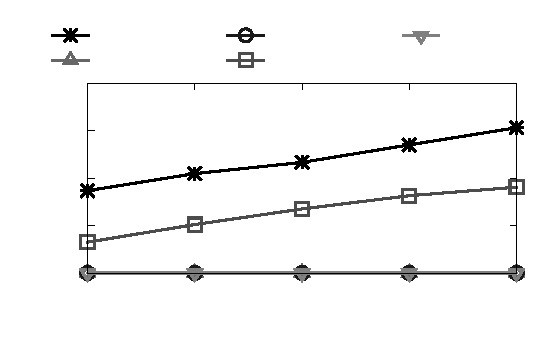
\includegraphics{fig1}}%
    \gplfronttext
  \end{picture}%
\endgroup
}
    \caption{P4 and fat-tree ($\portsPerSwitch=8$)}
    \label{fig:normal_update:p4}
  \end{subfigure}
    \begin{subfigure}[b]{0.49\linewidth}
    \resizebox{\linewidth}{!}{% GNUPLOT: LaTeX picture with Postscript
\begingroup
  \fontfamily{Times-Roman}%
  \selectfont
  \makeatletter
  \providecommand\color[2][]{%
    \GenericError{(gnuplot) \space\space\space\@spaces}{%
      Package color not loaded in conjunction with
      terminal option `colourtext'%
    }{See the gnuplot documentation for explanation.%
    }{Either use 'blacktext' in gnuplot or load the package
      color.sty in LaTeX.}%
    \renewcommand\color[2][]{}%
  }%
  \providecommand\includegraphics[2][]{%
    \GenericError{(gnuplot) \space\space\space\@spaces}{%
      Package graphicx or graphics not loaded%
    }{See the gnuplot documentation for explanation.%
    }{The gnuplot epslatex terminal needs graphicx.sty or graphics.sty.}%
    \renewcommand\includegraphics[2][]{}%
  }%
  \providecommand\rotatebox[2]{#2}%
  \@ifundefined{ifGPcolor}{%
    \newif\ifGPcolor
    \GPcolortrue
  }{}%
  \@ifundefined{ifGPblacktext}{%
    \newif\ifGPblacktext
    \GPblacktexttrue
  }{}%
  % define a \g@addto@macro without @ in the name:
  \let\gplgaddtomacro\g@addto@macro
  % define empty templates for all commands taking text:
  \gdef\gplbacktext{}%
  \gdef\gplfronttext{}%
  \makeatother
  \ifGPblacktext
    % no textcolor at all
    \def\colorrgb#1{}%
    \def\colorgray#1{}%
  \else
    % gray or color?
    \ifGPcolor
      \def\colorrgb#1{\color[rgb]{#1}}%
      \def\colorgray#1{\color[gray]{#1}}%
      \expandafter\def\csname LTw\endcsname{\color{white}}%
      \expandafter\def\csname LTb\endcsname{\color{black}}%
      \expandafter\def\csname LTa\endcsname{\color{black}}%
      \expandafter\def\csname LT0\endcsname{\color[rgb]{1,0,0}}%
      \expandafter\def\csname LT1\endcsname{\color[rgb]{0,1,0}}%
      \expandafter\def\csname LT2\endcsname{\color[rgb]{0,0,1}}%
      \expandafter\def\csname LT3\endcsname{\color[rgb]{1,0,1}}%
      \expandafter\def\csname LT4\endcsname{\color[rgb]{0,1,1}}%
      \expandafter\def\csname LT5\endcsname{\color[rgb]{1,1,0}}%
      \expandafter\def\csname LT6\endcsname{\color[rgb]{0,0,0}}%
      \expandafter\def\csname LT7\endcsname{\color[rgb]{1,0.3,0}}%
      \expandafter\def\csname LT8\endcsname{\color[rgb]{0.5,0.5,0.5}}%
    \else
      % gray
      \def\colorrgb#1{\color{black}}%
      \def\colorgray#1{\color[gray]{#1}}%
      \expandafter\def\csname LTw\endcsname{\color{white}}%
      \expandafter\def\csname LTb\endcsname{\color{black}}%
      \expandafter\def\csname LTa\endcsname{\color{black}}%
      \expandafter\def\csname LT0\endcsname{\color{black}}%
      \expandafter\def\csname LT1\endcsname{\color{black}}%
      \expandafter\def\csname LT2\endcsname{\color{black}}%
      \expandafter\def\csname LT3\endcsname{\color{black}}%
      \expandafter\def\csname LT4\endcsname{\color{black}}%
      \expandafter\def\csname LT5\endcsname{\color{black}}%
      \expandafter\def\csname LT6\endcsname{\color{black}}%
      \expandafter\def\csname LT7\endcsname{\color{black}}%
      \expandafter\def\csname LT8\endcsname{\color{black}}%
    \fi
  \fi
    \setlength{\unitlength}{0.0500bp}%
    \ifx\gptboxheight\undefined%
      \newlength{\gptboxheight}%
      \newlength{\gptboxwidth}%
      \newsavebox{\gptboxtext}%
    \fi%
    \setlength{\fboxrule}{0.5pt}%
    \setlength{\fboxsep}{1pt}%
\begin{picture}(4896.00,3024.00)%
    \gplgaddtomacro\gplbacktext{%
      \csname LTb\endcsname%
      \put(560,560){\makebox(0,0)[r]{\strut{}$0$}}%
      \put(560,1168){\makebox(0,0)[r]{\strut{}$20$}}%
      \put(560,1775){\makebox(0,0)[r]{\strut{}$40$}}%
      \put(560,2383){\makebox(0,0)[r]{\strut{}$60$}}%
      \put(680,360){\makebox(0,0){\strut{}$600$}}%
      \put(1710,360){\makebox(0,0){\strut{}$700$}}%
      \put(2740,360){\makebox(0,0){\strut{}$800$}}%
      \put(3769,360){\makebox(0,0){\strut{}$900$}}%
      \put(4799,360){\makebox(0,0){\strut{}$1000$}}%
    }%
    \gplgaddtomacro\gplfronttext{%
      \csname LTb\endcsname%
      \put(160,1471){\rotatebox{-270}{\makebox(0,0){\strut{}\ylabel}}}%
      \put(2739,140){\makebox(0,0){\strut{}\xlabel}}%
      \csname LTb\endcsname%
      \put(818,2841){\makebox(0,0)[l]{\strut{}\org}}%
      \csname LTb\endcsname%
      \put(818,2601){\makebox(0,0)[l]{\strut{}\sys}}%
      \csname LTb\endcsname%
      \put(2501,2841){\makebox(0,0)[l]{\strut{}\cu}}%
      \csname LTb\endcsname%
      \put(2501,2601){\makebox(0,0)[l]{\strut{}\coconut}}%
      \csname LTb\endcsname%
      \put(4184,2841){\makebox(0,0)[l]{\strut{}\tsu}}%
    }%
    \gplbacktext
    \put(0,0){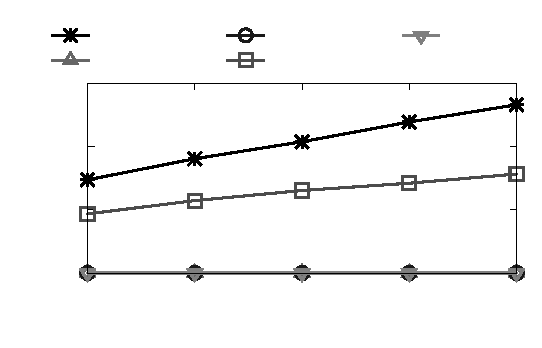
\includegraphics{loss}}%
    \gplfronttext
  \end{picture}%
\endgroup
}
    \caption{OVS and fat-tree ($\portsPerSwitch=8$)}
    \label{fig:normal_update:openvswitch}
  \end{subfigure}
\caption{Packet loss during normal update.  Each data point is an
average of 100 runs.}
\label{fig:normal_update}
\end{figure}

We measured the number of lost packets based on different packet
sending rates when pushing updates to the switches concurrently to
change the paths of packets in the fat-tree topology
($\portsPerSwitch=8$).  As shown in \figref{fig:normal_update}, our
protocol (SCC), TSU, and CU incur no packet loss because these two
mechanisms maintain black-hole freedom.  In addition, we set the TTL
of each packet to be twice its old path length plus its new path
length. So no packet loss also indicates bounded looping, since the
packet will be dropped if its TTL reaches zero.  In contrast, the
normal deployment without any consistent update mechanism and COCONUT
dropped packets because they do not prevent the case where a switch
forwards packets using an old rule to a switch that is not on the new
path for this packet and that has already deleted (or deprecated) its
old rule.  The ``original'' deployment approach also drops packets in
other cases that COCONUT addresses (and that CU, TSU, and SCC also
address).


\subsection{Packet Loss During Link Failure}
\label{sec:eval:link-failure}

\begin{figure}[h]
\centering
  \begin{subfigure}[b]{0.49\linewidth}
    \resizebox{\linewidth}{!}{% GNUPLOT: LaTeX picture with Postscript
\begingroup
  \fontfamily{Times-Roman}%
  \selectfont
  \makeatletter
  \providecommand\color[2][]{%
    \GenericError{(gnuplot) \space\space\space\@spaces}{%
      Package color not loaded in conjunction with
      terminal option `colourtext'%
    }{See the gnuplot documentation for explanation.%
    }{Either use 'blacktext' in gnuplot or load the package
      color.sty in LaTeX.}%
    \renewcommand\color[2][]{}%
  }%
  \providecommand\includegraphics[2][]{%
    \GenericError{(gnuplot) \space\space\space\@spaces}{%
      Package graphicx or graphics not loaded%
    }{See the gnuplot documentation for explanation.%
    }{The gnuplot epslatex terminal needs graphicx.sty or graphics.sty.}%
    \renewcommand\includegraphics[2][]{}%
  }%
  \providecommand\rotatebox[2]{#2}%
  \@ifundefined{ifGPcolor}{%
    \newif\ifGPcolor
    \GPcolortrue
  }{}%
  \@ifundefined{ifGPblacktext}{%
    \newif\ifGPblacktext
    \GPblacktexttrue
  }{}%
  % define a \g@addto@macro without @ in the name:
  \let\gplgaddtomacro\g@addto@macro
  % define empty templates for all commands taking text:
  \gdef\gplbacktext{}%
  \gdef\gplfronttext{}%
  \makeatother
  \ifGPblacktext
    % no textcolor at all
    \def\colorrgb#1{}%
    \def\colorgray#1{}%
  \else
    % gray or color?
    \ifGPcolor
      \def\colorrgb#1{\color[rgb]{#1}}%
      \def\colorgray#1{\color[gray]{#1}}%
      \expandafter\def\csname LTw\endcsname{\color{white}}%
      \expandafter\def\csname LTb\endcsname{\color{black}}%
      \expandafter\def\csname LTa\endcsname{\color{black}}%
      \expandafter\def\csname LT0\endcsname{\color[rgb]{1,0,0}}%
      \expandafter\def\csname LT1\endcsname{\color[rgb]{0,1,0}}%
      \expandafter\def\csname LT2\endcsname{\color[rgb]{0,0,1}}%
      \expandafter\def\csname LT3\endcsname{\color[rgb]{1,0,1}}%
      \expandafter\def\csname LT4\endcsname{\color[rgb]{0,1,1}}%
      \expandafter\def\csname LT5\endcsname{\color[rgb]{1,1,0}}%
      \expandafter\def\csname LT6\endcsname{\color[rgb]{0,0,0}}%
      \expandafter\def\csname LT7\endcsname{\color[rgb]{1,0.3,0}}%
      \expandafter\def\csname LT8\endcsname{\color[rgb]{0.5,0.5,0.5}}%
    \else
      % gray
      \def\colorrgb#1{\color{black}}%
      \def\colorgray#1{\color[gray]{#1}}%
      \expandafter\def\csname LTw\endcsname{\color{white}}%
      \expandafter\def\csname LTb\endcsname{\color{black}}%
      \expandafter\def\csname LTa\endcsname{\color{black}}%
      \expandafter\def\csname LT0\endcsname{\color{black}}%
      \expandafter\def\csname LT1\endcsname{\color{black}}%
      \expandafter\def\csname LT2\endcsname{\color{black}}%
      \expandafter\def\csname LT3\endcsname{\color{black}}%
      \expandafter\def\csname LT4\endcsname{\color{black}}%
      \expandafter\def\csname LT5\endcsname{\color{black}}%
      \expandafter\def\csname LT6\endcsname{\color{black}}%
      \expandafter\def\csname LT7\endcsname{\color{black}}%
      \expandafter\def\csname LT8\endcsname{\color{black}}%
    \fi
  \fi
    \setlength{\unitlength}{0.0500bp}%
    \ifx\gptboxheight\undefined%
      \newlength{\gptboxheight}%
      \newlength{\gptboxwidth}%
      \newsavebox{\gptboxtext}%
    \fi%
    \setlength{\fboxrule}{0.5pt}%
    \setlength{\fboxsep}{1pt}%
\begin{picture}(4896.00,3024.00)%
    \gplgaddtomacro\gplbacktext{%
      \csname LTb\endcsname%
      \put(680,560){\makebox(0,0)[r]{\strut{}$0$}}%
      \put(680,925){\makebox(0,0)[r]{\strut{}$100$}}%
      \put(680,1289){\makebox(0,0)[r]{\strut{}$200$}}%
      \put(680,1654){\makebox(0,0)[r]{\strut{}$300$}}%
      \put(680,2018){\makebox(0,0)[r]{\strut{}$400$}}%
      \put(680,2383){\makebox(0,0)[r]{\strut{}$500$}}%
      \put(800,360){\makebox(0,0){\strut{}$600$}}%
      \put(1800,360){\makebox(0,0){\strut{}$700$}}%
      \put(2800,360){\makebox(0,0){\strut{}$800$}}%
      \put(3799,360){\makebox(0,0){\strut{}$900$}}%
      \put(4799,360){\makebox(0,0){\strut{}$1000$}}%
    }%
    \gplgaddtomacro\gplfronttext{%
      \csname LTb\endcsname%
      \put(160,1471){\rotatebox{-270}{\makebox(0,0){\strut{}\ylabel}}}%
      \put(2799,140){\makebox(0,0){\strut{}\xlabel}}%
      \csname LTb\endcsname%
      \put(878,2841){\makebox(0,0)[l]{\strut{}\org}}%
      \csname LTb\endcsname%
      \put(878,2601){\makebox(0,0)[l]{\strut{}\sys}}%
      \csname LTb\endcsname%
      \put(2561,2841){\makebox(0,0)[l]{\strut{}\cu}}%
      \csname LTb\endcsname%
      \put(2561,2601){\makebox(0,0)[l]{\strut{}\coconut}}%
      \csname LTb\endcsname%
      \put(4244,2841){\makebox(0,0)[l]{\strut{}\tsu}}%
    }%
    \gplbacktext
    \put(0,0){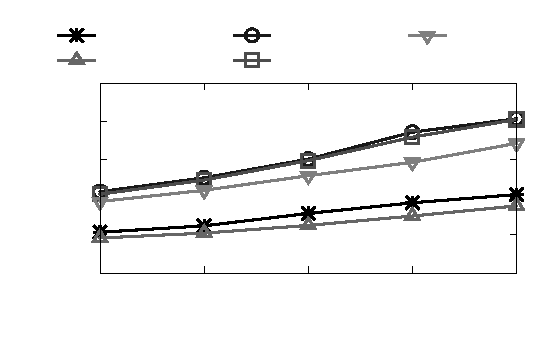
\includegraphics{fig2}}%
    \gplfronttext
  \end{picture}%
\endgroup
}
    \caption{P4 and fat-tree ($\portsPerSwitch=8$)}
    \label{fig:link_failure:fat_tree-p4}
  \end{subfigure}
    \begin{subfigure}[b]{0.49\linewidth}
    \resizebox{\linewidth}{!}{% GNUPLOT: LaTeX picture with Postscript
\begingroup
  \fontfamily{Times-Roman}%
  \selectfont
  \makeatletter
  \providecommand\color[2][]{%
    \GenericError{(gnuplot) \space\space\space\@spaces}{%
      Package color not loaded in conjunction with
      terminal option `colourtext'%
    }{See the gnuplot documentation for explanation.%
    }{Either use 'blacktext' in gnuplot or load the package
      color.sty in LaTeX.}%
    \renewcommand\color[2][]{}%
  }%
  \providecommand\includegraphics[2][]{%
    \GenericError{(gnuplot) \space\space\space\@spaces}{%
      Package graphicx or graphics not loaded%
    }{See the gnuplot documentation for explanation.%
    }{The gnuplot epslatex terminal needs graphicx.sty or graphics.sty.}%
    \renewcommand\includegraphics[2][]{}%
  }%
  \providecommand\rotatebox[2]{#2}%
  \@ifundefined{ifGPcolor}{%
    \newif\ifGPcolor
    \GPcolortrue
  }{}%
  \@ifundefined{ifGPblacktext}{%
    \newif\ifGPblacktext
    \GPblacktexttrue
  }{}%
  % define a \g@addto@macro without @ in the name:
  \let\gplgaddtomacro\g@addto@macro
  % define empty templates for all commands taking text:
  \gdef\gplbacktext{}%
  \gdef\gplfronttext{}%
  \makeatother
  \ifGPblacktext
    % no textcolor at all
    \def\colorrgb#1{}%
    \def\colorgray#1{}%
  \else
    % gray or color?
    \ifGPcolor
      \def\colorrgb#1{\color[rgb]{#1}}%
      \def\colorgray#1{\color[gray]{#1}}%
      \expandafter\def\csname LTw\endcsname{\color{white}}%
      \expandafter\def\csname LTb\endcsname{\color{black}}%
      \expandafter\def\csname LTa\endcsname{\color{black}}%
      \expandafter\def\csname LT0\endcsname{\color[rgb]{1,0,0}}%
      \expandafter\def\csname LT1\endcsname{\color[rgb]{0,1,0}}%
      \expandafter\def\csname LT2\endcsname{\color[rgb]{0,0,1}}%
      \expandafter\def\csname LT3\endcsname{\color[rgb]{1,0,1}}%
      \expandafter\def\csname LT4\endcsname{\color[rgb]{0,1,1}}%
      \expandafter\def\csname LT5\endcsname{\color[rgb]{1,1,0}}%
      \expandafter\def\csname LT6\endcsname{\color[rgb]{0,0,0}}%
      \expandafter\def\csname LT7\endcsname{\color[rgb]{1,0.3,0}}%
      \expandafter\def\csname LT8\endcsname{\color[rgb]{0.5,0.5,0.5}}%
    \else
      % gray
      \def\colorrgb#1{\color{black}}%
      \def\colorgray#1{\color[gray]{#1}}%
      \expandafter\def\csname LTw\endcsname{\color{white}}%
      \expandafter\def\csname LTb\endcsname{\color{black}}%
      \expandafter\def\csname LTa\endcsname{\color{black}}%
      \expandafter\def\csname LT0\endcsname{\color{black}}%
      \expandafter\def\csname LT1\endcsname{\color{black}}%
      \expandafter\def\csname LT2\endcsname{\color{black}}%
      \expandafter\def\csname LT3\endcsname{\color{black}}%
      \expandafter\def\csname LT4\endcsname{\color{black}}%
      \expandafter\def\csname LT5\endcsname{\color{black}}%
      \expandafter\def\csname LT6\endcsname{\color{black}}%
      \expandafter\def\csname LT7\endcsname{\color{black}}%
      \expandafter\def\csname LT8\endcsname{\color{black}}%
    \fi
  \fi
    \setlength{\unitlength}{0.0500bp}%
    \ifx\gptboxheight\undefined%
      \newlength{\gptboxheight}%
      \newlength{\gptboxwidth}%
      \newsavebox{\gptboxtext}%
    \fi%
    \setlength{\fboxrule}{0.5pt}%
    \setlength{\fboxsep}{1pt}%
\begin{picture}(4896.00,3024.00)%
    \gplgaddtomacro\gplbacktext{%
      \csname LTb\endcsname%
      \put(680,560){\makebox(0,0)[r]{\strut{}$0$}}%
      \put(680,1016){\makebox(0,0)[r]{\strut{}$100$}}%
      \put(680,1472){\makebox(0,0)[r]{\strut{}$200$}}%
      \put(680,1927){\makebox(0,0)[r]{\strut{}$300$}}%
      \put(680,2383){\makebox(0,0)[r]{\strut{}$400$}}%
      \put(800,360){\makebox(0,0){\strut{}$600$}}%
      \put(1800,360){\makebox(0,0){\strut{}$700$}}%
      \put(2800,360){\makebox(0,0){\strut{}$800$}}%
      \put(3799,360){\makebox(0,0){\strut{}$900$}}%
      \put(4799,360){\makebox(0,0){\strut{}$1000$}}%
    }%
    \gplgaddtomacro\gplfronttext{%
      \csname LTb\endcsname%
      \put(160,1471){\rotatebox{-270}{\makebox(0,0){\strut{}\ylabel}}}%
      \put(2799,140){\makebox(0,0){\strut{}\xlabel}}%
      \csname LTb\endcsname%
      \put(878,2841){\makebox(0,0)[l]{\strut{}\org}}%
      \csname LTb\endcsname%
      \put(878,2601){\makebox(0,0)[l]{\strut{}\sys}}%
      \csname LTb\endcsname%
      \put(2561,2841){\makebox(0,0)[l]{\strut{}\cu}}%
      \csname LTb\endcsname%
      \put(2561,2601){\makebox(0,0)[l]{\strut{}\coconut}}%
      \csname LTb\endcsname%
      \put(4244,2841){\makebox(0,0)[l]{\strut{}\tsu}}%
    }%
    \gplbacktext
    \put(0,0){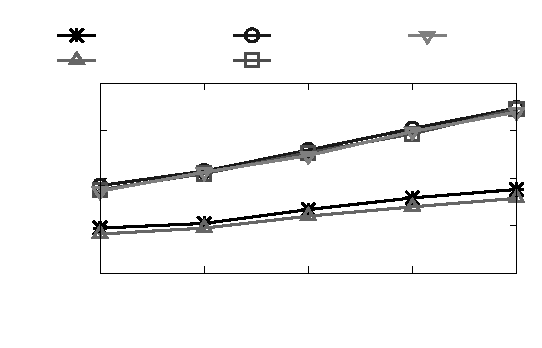
\includegraphics{loss2}}%
    \gplfronttext
  \end{picture}%
\endgroup
}
    \caption{OVS and fat-tree ($\portsPerSwitch=8$)}
    \label{fig:link_failure:fat_tree-ovs}
  \end{subfigure}
    \begin{subfigure}[b]{0.49\linewidth}
    \resizebox{\linewidth}{!}{% GNUPLOT: LaTeX picture with Postscript
\begingroup
  \fontfamily{Times-Roman}%
  \selectfont
  \makeatletter
  \providecommand\color[2][]{%
    \GenericError{(gnuplot) \space\space\space\@spaces}{%
      Package color not loaded in conjunction with
      terminal option `colourtext'%
    }{See the gnuplot documentation for explanation.%
    }{Either use 'blacktext' in gnuplot or load the package
      color.sty in LaTeX.}%
    \renewcommand\color[2][]{}%
  }%
  \providecommand\includegraphics[2][]{%
    \GenericError{(gnuplot) \space\space\space\@spaces}{%
      Package graphicx or graphics not loaded%
    }{See the gnuplot documentation for explanation.%
    }{The gnuplot epslatex terminal needs graphicx.sty or graphics.sty.}%
    \renewcommand\includegraphics[2][]{}%
  }%
  \providecommand\rotatebox[2]{#2}%
  \@ifundefined{ifGPcolor}{%
    \newif\ifGPcolor
    \GPcolortrue
  }{}%
  \@ifundefined{ifGPblacktext}{%
    \newif\ifGPblacktext
    \GPblacktexttrue
  }{}%
  % define a \g@addto@macro without @ in the name:
  \let\gplgaddtomacro\g@addto@macro
  % define empty templates for all commands taking text:
  \gdef\gplbacktext{}%
  \gdef\gplfronttext{}%
  \makeatother
  \ifGPblacktext
    % no textcolor at all
    \def\colorrgb#1{}%
    \def\colorgray#1{}%
  \else
    % gray or color?
    \ifGPcolor
      \def\colorrgb#1{\color[rgb]{#1}}%
      \def\colorgray#1{\color[gray]{#1}}%
      \expandafter\def\csname LTw\endcsname{\color{white}}%
      \expandafter\def\csname LTb\endcsname{\color{black}}%
      \expandafter\def\csname LTa\endcsname{\color{black}}%
      \expandafter\def\csname LT0\endcsname{\color[rgb]{1,0,0}}%
      \expandafter\def\csname LT1\endcsname{\color[rgb]{0,1,0}}%
      \expandafter\def\csname LT2\endcsname{\color[rgb]{0,0,1}}%
      \expandafter\def\csname LT3\endcsname{\color[rgb]{1,0,1}}%
      \expandafter\def\csname LT4\endcsname{\color[rgb]{0,1,1}}%
      \expandafter\def\csname LT5\endcsname{\color[rgb]{1,1,0}}%
      \expandafter\def\csname LT6\endcsname{\color[rgb]{0,0,0}}%
      \expandafter\def\csname LT7\endcsname{\color[rgb]{1,0.3,0}}%
      \expandafter\def\csname LT8\endcsname{\color[rgb]{0.5,0.5,0.5}}%
    \else
      % gray
      \def\colorrgb#1{\color{black}}%
      \def\colorgray#1{\color[gray]{#1}}%
      \expandafter\def\csname LTw\endcsname{\color{white}}%
      \expandafter\def\csname LTb\endcsname{\color{black}}%
      \expandafter\def\csname LTa\endcsname{\color{black}}%
      \expandafter\def\csname LT0\endcsname{\color{black}}%
      \expandafter\def\csname LT1\endcsname{\color{black}}%
      \expandafter\def\csname LT2\endcsname{\color{black}}%
      \expandafter\def\csname LT3\endcsname{\color{black}}%
      \expandafter\def\csname LT4\endcsname{\color{black}}%
      \expandafter\def\csname LT5\endcsname{\color{black}}%
      \expandafter\def\csname LT6\endcsname{\color{black}}%
      \expandafter\def\csname LT7\endcsname{\color{black}}%
      \expandafter\def\csname LT8\endcsname{\color{black}}%
    \fi
  \fi
    \setlength{\unitlength}{0.0500bp}%
    \ifx\gptboxheight\undefined%
      \newlength{\gptboxheight}%
      \newlength{\gptboxwidth}%
      \newsavebox{\gptboxtext}%
    \fi%
    \setlength{\fboxrule}{0.5pt}%
    \setlength{\fboxsep}{1pt}%
\begin{picture}(4896.00,3024.00)%
    \gplgaddtomacro\gplbacktext{%
      \csname LTb\endcsname%
      \put(680,560){\makebox(0,0)[r]{\strut{}$0$}}%
      \put(680,925){\makebox(0,0)[r]{\strut{}$100$}}%
      \put(680,1289){\makebox(0,0)[r]{\strut{}$200$}}%
      \put(680,1654){\makebox(0,0)[r]{\strut{}$300$}}%
      \put(680,2018){\makebox(0,0)[r]{\strut{}$400$}}%
      \put(680,2383){\makebox(0,0)[r]{\strut{}$500$}}%
      \put(800,360){\makebox(0,0){\strut{}$600$}}%
      \put(1800,360){\makebox(0,0){\strut{}$700$}}%
      \put(2800,360){\makebox(0,0){\strut{}$800$}}%
      \put(3799,360){\makebox(0,0){\strut{}$900$}}%
      \put(4799,360){\makebox(0,0){\strut{}$1000$}}%
    }%
    \gplgaddtomacro\gplfronttext{%
      \csname LTb\endcsname%
      \put(160,1471){\rotatebox{-270}{\makebox(0,0){\strut{}\ylabel}}}%
      \put(2799,140){\makebox(0,0){\strut{}\xlabel}}%
      \csname LTb\endcsname%
      \put(878,2841){\makebox(0,0)[l]{\strut{}\org}}%
      \csname LTb\endcsname%
      \put(878,2601){\makebox(0,0)[l]{\strut{}\sys}}%
      \csname LTb\endcsname%
      \put(2561,2841){\makebox(0,0)[l]{\strut{}\cu}}%
      \csname LTb\endcsname%
      \put(2561,2601){\makebox(0,0)[l]{\strut{}\coconut}}%
      \csname LTb\endcsname%
      \put(4244,2841){\makebox(0,0)[l]{\strut{}\tsu}}%
    }%
    \gplbacktext
    \put(0,0){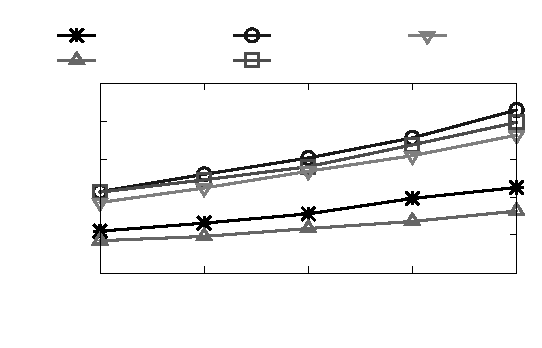
\includegraphics{fig5}}%
    \gplfronttext
  \end{picture}%
\endgroup
}
    \caption{P4 and DFN topology}
    \label{fig:link_failure:dfn}
  \end{subfigure}
  \caption{Packet loss during link failure.  Each data point is an
  average of 100 runs.}
  \label{fig:link_failure}
\end{figure}

In the tests reported in this section, we broke one randomly chosen
link of some existing path, forcing a new epoch with new paths for
the flows traversing that link.  During the delay to update the network with the new
paths, packets on those flows were lost.  For the $\portsPerSwitch=8$
fat-tree topology
(\figrefs{fig:link_failure:fat_tree-p4}{fig:link_failure:fat_tree-ovs}),
the response time included rule generation (i.e., the delay for
executing our algorithm), while we pre-computed the rules for the DFN
topology (\figref{fig:link_failure:dfn}).  The DFN results for Open
vSwitch are similar to those for P4 and so are omitted for brevity.
As we can see in \figref{fig:link_failure}, SCC dropped fewer packets
than COCONUT, TSU, and CU because our protocol has smaller delay to
put the new configuration in place. Specifically, in SCC, new rules
can be applied as soon as they are installed in the switch.  However,
CU and COCONUT require that updated rules reach all switches on the
new paths before any of them can start to be used to route packets, and
TSU deploys new rules over multiple steps. Also, SCC outperforms the
``original'' deployment due to the consistency that SCC offers; e.g.,
SCC prevents packets forwarded using a new rule from then being
matched to an old rule or otherwise dropped.

\subsection{Rule Deployment Time}
\label{sec:eval:deployment}

In the tests reported in this section, we measured the deployment time
of rule updates, including both the new rule installation and old rule
cleanup (and, in our case, send-back rule cleanup).  Each epoch in
these tests involved one path change, and \figref{fig:completion_time}
shows the distribution of rule deployment times for 100 such epochs
for the fat-tree topology ($\portsPerSwitch=8$).  SCC rule deployment
is considerably faster than TSU, CU and COCONUT, with the vast
majority of the 100 SCC deployments completing before even a minority
of the TSU and CU deployments and well before any COCONUT deployments.
Total completion time of SCC is only slightly larger than for the
``original'' protocol, owing to extra rule cleanup.

\begin{figure}[h]
\centering
  \begin{subfigure}[b]{0.49\linewidth}
    \resizebox{\linewidth}{!}{% GNUPLOT: LaTeX picture with Postscript
\begingroup
  \fontfamily{Times-Roman}%
  \selectfont
  \makeatletter
  \providecommand\color[2][]{%
    \GenericError{(gnuplot) \space\space\space\@spaces}{%
      Package color not loaded in conjunction with
      terminal option `colourtext'%
    }{See the gnuplot documentation for explanation.%
    }{Either use 'blacktext' in gnuplot or load the package
      color.sty in LaTeX.}%
    \renewcommand\color[2][]{}%
  }%
  \providecommand\includegraphics[2][]{%
    \GenericError{(gnuplot) \space\space\space\@spaces}{%
      Package graphicx or graphics not loaded%
    }{See the gnuplot documentation for explanation.%
    }{The gnuplot epslatex terminal needs graphicx.sty or graphics.sty.}%
    \renewcommand\includegraphics[2][]{}%
  }%
  \providecommand\rotatebox[2]{#2}%
  \@ifundefined{ifGPcolor}{%
    \newif\ifGPcolor
    \GPcolortrue
  }{}%
  \@ifundefined{ifGPblacktext}{%
    \newif\ifGPblacktext
    \GPblacktexttrue
  }{}%
  % define a \g@addto@macro without @ in the name:
  \let\gplgaddtomacro\g@addto@macro
  % define empty templates for all commands taking text:
  \gdef\gplbacktext{}%
  \gdef\gplfronttext{}%
  \makeatother
  \ifGPblacktext
    % no textcolor at all
    \def\colorrgb#1{}%
    \def\colorgray#1{}%
  \else
    % gray or color?
    \ifGPcolor
      \def\colorrgb#1{\color[rgb]{#1}}%
      \def\colorgray#1{\color[gray]{#1}}%
      \expandafter\def\csname LTw\endcsname{\color{white}}%
      \expandafter\def\csname LTb\endcsname{\color{black}}%
      \expandafter\def\csname LTa\endcsname{\color{black}}%
      \expandafter\def\csname LT0\endcsname{\color[rgb]{1,0,0}}%
      \expandafter\def\csname LT1\endcsname{\color[rgb]{0,1,0}}%
      \expandafter\def\csname LT2\endcsname{\color[rgb]{0,0,1}}%
      \expandafter\def\csname LT3\endcsname{\color[rgb]{1,0,1}}%
      \expandafter\def\csname LT4\endcsname{\color[rgb]{0,1,1}}%
      \expandafter\def\csname LT5\endcsname{\color[rgb]{1,1,0}}%
      \expandafter\def\csname LT6\endcsname{\color[rgb]{0,0,0}}%
      \expandafter\def\csname LT7\endcsname{\color[rgb]{1,0.3,0}}%
      \expandafter\def\csname LT8\endcsname{\color[rgb]{0.5,0.5,0.5}}%
    \else
      % gray
      \def\colorrgb#1{\color{black}}%
      \def\colorgray#1{\color[gray]{#1}}%
      \expandafter\def\csname LTw\endcsname{\color{white}}%
      \expandafter\def\csname LTb\endcsname{\color{black}}%
      \expandafter\def\csname LTa\endcsname{\color{black}}%
      \expandafter\def\csname LT0\endcsname{\color{black}}%
      \expandafter\def\csname LT1\endcsname{\color{black}}%
      \expandafter\def\csname LT2\endcsname{\color{black}}%
      \expandafter\def\csname LT3\endcsname{\color{black}}%
      \expandafter\def\csname LT4\endcsname{\color{black}}%
      \expandafter\def\csname LT5\endcsname{\color{black}}%
      \expandafter\def\csname LT6\endcsname{\color{black}}%
      \expandafter\def\csname LT7\endcsname{\color{black}}%
      \expandafter\def\csname LT8\endcsname{\color{black}}%
    \fi
  \fi
    \setlength{\unitlength}{0.0500bp}%
    \ifx\gptboxheight\undefined%
      \newlength{\gptboxheight}%
      \newlength{\gptboxwidth}%
      \newsavebox{\gptboxtext}%
    \fi%
    \setlength{\fboxrule}{0.5pt}%
    \setlength{\fboxsep}{1pt}%
\begin{picture}(4896.00,3024.00)%
    \gplgaddtomacro\gplbacktext{%
      \csname LTb\endcsname%
      \put(540,975){\makebox(0,0)[r]{\strut{}$0.2$}}%
      \csname LTb\endcsname%
      \put(540,1327){\makebox(0,0)[r]{\strut{}$0.4$}}%
      \csname LTb\endcsname%
      \put(540,1679){\makebox(0,0)[r]{\strut{}$0.6$}}%
      \csname LTb\endcsname%
      \put(540,2031){\makebox(0,0)[r]{\strut{}$0.8$}}%
      \csname LTb\endcsname%
      \put(540,2383){\makebox(0,0)[r]{\strut{}$1$}}%
      \csname LTb\endcsname%
      \put(660,440){\makebox(0,0){\strut{}$0$}}%
      \csname LTb\endcsname%
      \put(1036,440){\makebox(0,0){\strut{}$0.1$}}%
      \csname LTb\endcsname%
      \put(1413,440){\makebox(0,0){\strut{}$0.2$}}%
      \csname LTb\endcsname%
      \put(1789,440){\makebox(0,0){\strut{}$0.3$}}%
      \csname LTb\endcsname%
      \put(2165,440){\makebox(0,0){\strut{}$0.4$}}%
      \csname LTb\endcsname%
      \put(2541,440){\makebox(0,0){\strut{}$0.5$}}%
      \csname LTb\endcsname%
      \put(2918,440){\makebox(0,0){\strut{}$0.6$}}%
      \csname LTb\endcsname%
      \put(3294,440){\makebox(0,0){\strut{}$0.7$}}%
      \csname LTb\endcsname%
      \put(3670,440){\makebox(0,0){\strut{}$0.8$}}%
      \csname LTb\endcsname%
      \put(4046,440){\makebox(0,0){\strut{}$0.9$}}%
      \csname LTb\endcsname%
      \put(4423,440){\makebox(0,0){\strut{}$1$}}%
      \csname LTb\endcsname%
      \put(4799,440){\makebox(0,0){\strut{}$1.1$}}%
    }%
    \gplgaddtomacro\gplfronttext{%
      \csname LTb\endcsname%
      \put(200,1511){\rotatebox{-270}{\makebox(0,0){\strut{}}}}%
      \put(2729,140){\makebox(0,0){\strut{}\updateTime(s)}}%
      \csname LTb\endcsname%
      \put(808,2841){\makebox(0,0)[l]{\strut{}\org}}%
      \csname LTb\endcsname%
      \put(808,2601){\makebox(0,0)[l]{\strut{}\sys}}%
      \csname LTb\endcsname%
      \put(2491,2841){\makebox(0,0)[l]{\strut{}\cu}}%
      \csname LTb\endcsname%
      \put(2491,2601){\makebox(0,0)[l]{\strut{}\coconut}}%
      \csname LTb\endcsname%
      \put(4174,2841){\makebox(0,0)[l]{\strut{}\tsu}}%
    }%
    \gplbacktext
    \put(0,0){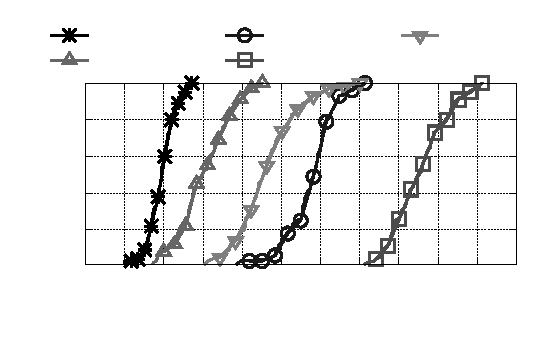
\includegraphics{p4CDF}}%
    \gplfronttext
  \end{picture}%
\endgroup
}
    \caption{P4 and fat-tree ($\portsPerSwitch=8$)}
    \label{fig:completion_time:p4}
  \end{subfigure}
    \begin{subfigure}[b]{0.49\linewidth}
    \resizebox{\linewidth}{!}{% GNUPLOT: LaTeX picture with Postscript
\begingroup
  \fontfamily{Times-Roman}%
  \selectfont
  \makeatletter
  \providecommand\color[2][]{%
    \GenericError{(gnuplot) \space\space\space\@spaces}{%
      Package color not loaded in conjunction with
      terminal option `colourtext'%
    }{See the gnuplot documentation for explanation.%
    }{Either use 'blacktext' in gnuplot or load the package
      color.sty in LaTeX.}%
    \renewcommand\color[2][]{}%
  }%
  \providecommand\includegraphics[2][]{%
    \GenericError{(gnuplot) \space\space\space\@spaces}{%
      Package graphicx or graphics not loaded%
    }{See the gnuplot documentation for explanation.%
    }{The gnuplot epslatex terminal needs graphicx.sty or graphics.sty.}%
    \renewcommand\includegraphics[2][]{}%
  }%
  \providecommand\rotatebox[2]{#2}%
  \@ifundefined{ifGPcolor}{%
    \newif\ifGPcolor
    \GPcolortrue
  }{}%
  \@ifundefined{ifGPblacktext}{%
    \newif\ifGPblacktext
    \GPblacktexttrue
  }{}%
  % define a \g@addto@macro without @ in the name:
  \let\gplgaddtomacro\g@addto@macro
  % define empty templates for all commands taking text:
  \gdef\gplbacktext{}%
  \gdef\gplfronttext{}%
  \makeatother
  \ifGPblacktext
    % no textcolor at all
    \def\colorrgb#1{}%
    \def\colorgray#1{}%
  \else
    % gray or color?
    \ifGPcolor
      \def\colorrgb#1{\color[rgb]{#1}}%
      \def\colorgray#1{\color[gray]{#1}}%
      \expandafter\def\csname LTw\endcsname{\color{white}}%
      \expandafter\def\csname LTb\endcsname{\color{black}}%
      \expandafter\def\csname LTa\endcsname{\color{black}}%
      \expandafter\def\csname LT0\endcsname{\color[rgb]{1,0,0}}%
      \expandafter\def\csname LT1\endcsname{\color[rgb]{0,1,0}}%
      \expandafter\def\csname LT2\endcsname{\color[rgb]{0,0,1}}%
      \expandafter\def\csname LT3\endcsname{\color[rgb]{1,0,1}}%
      \expandafter\def\csname LT4\endcsname{\color[rgb]{0,1,1}}%
      \expandafter\def\csname LT5\endcsname{\color[rgb]{1,1,0}}%
      \expandafter\def\csname LT6\endcsname{\color[rgb]{0,0,0}}%
      \expandafter\def\csname LT7\endcsname{\color[rgb]{1,0.3,0}}%
      \expandafter\def\csname LT8\endcsname{\color[rgb]{0.5,0.5,0.5}}%
    \else
      % gray
      \def\colorrgb#1{\color{black}}%
      \def\colorgray#1{\color[gray]{#1}}%
      \expandafter\def\csname LTw\endcsname{\color{white}}%
      \expandafter\def\csname LTb\endcsname{\color{black}}%
      \expandafter\def\csname LTa\endcsname{\color{black}}%
      \expandafter\def\csname LT0\endcsname{\color{black}}%
      \expandafter\def\csname LT1\endcsname{\color{black}}%
      \expandafter\def\csname LT2\endcsname{\color{black}}%
      \expandafter\def\csname LT3\endcsname{\color{black}}%
      \expandafter\def\csname LT4\endcsname{\color{black}}%
      \expandafter\def\csname LT5\endcsname{\color{black}}%
      \expandafter\def\csname LT6\endcsname{\color{black}}%
      \expandafter\def\csname LT7\endcsname{\color{black}}%
      \expandafter\def\csname LT8\endcsname{\color{black}}%
    \fi
  \fi
    \setlength{\unitlength}{0.0500bp}%
    \ifx\gptboxheight\undefined%
      \newlength{\gptboxheight}%
      \newlength{\gptboxwidth}%
      \newsavebox{\gptboxtext}%
    \fi%
    \setlength{\fboxrule}{0.5pt}%
    \setlength{\fboxsep}{1pt}%
\begin{picture}(4896.00,3024.00)%
    \gplgaddtomacro\gplbacktext{%
      \csname LTb\endcsname%
      \put(540,975){\makebox(0,0)[r]{\strut{}$0.2$}}%
      \csname LTb\endcsname%
      \put(540,1327){\makebox(0,0)[r]{\strut{}$0.4$}}%
      \csname LTb\endcsname%
      \put(540,1679){\makebox(0,0)[r]{\strut{}$0.6$}}%
      \csname LTb\endcsname%
      \put(540,2031){\makebox(0,0)[r]{\strut{}$0.8$}}%
      \csname LTb\endcsname%
      \put(540,2383){\makebox(0,0)[r]{\strut{}$1$}}%
      \csname LTb\endcsname%
      \put(660,440){\makebox(0,0){\strut{}$0.1$}}%
      \csname LTb\endcsname%
      \put(1074,440){\makebox(0,0){\strut{}$0.2$}}%
      \csname LTb\endcsname%
      \put(1488,440){\makebox(0,0){\strut{}$0.3$}}%
      \csname LTb\endcsname%
      \put(1902,440){\makebox(0,0){\strut{}$0.4$}}%
      \csname LTb\endcsname%
      \put(2316,440){\makebox(0,0){\strut{}$0.5$}}%
      \csname LTb\endcsname%
      \put(2730,440){\makebox(0,0){\strut{}$0.6$}}%
      \csname LTb\endcsname%
      \put(3143,440){\makebox(0,0){\strut{}$0.7$}}%
      \csname LTb\endcsname%
      \put(3557,440){\makebox(0,0){\strut{}$0.8$}}%
      \csname LTb\endcsname%
      \put(3971,440){\makebox(0,0){\strut{}$0.9$}}%
      \csname LTb\endcsname%
      \put(4385,440){\makebox(0,0){\strut{}$1$}}%
      \csname LTb\endcsname%
      \put(4799,440){\makebox(0,0){\strut{}$1.1$}}%
    }%
    \gplgaddtomacro\gplfronttext{%
      \csname LTb\endcsname%
      \put(200,1511){\rotatebox{-270}{\makebox(0,0){\strut{}}}}%
      \put(2729,140){\makebox(0,0){\strut{}\updateTime(s)}}%
      \csname LTb\endcsname%
      \put(808,2841){\makebox(0,0)[l]{\strut{}\org}}%
      \csname LTb\endcsname%
      \put(808,2601){\makebox(0,0)[l]{\strut{}\sys}}%
      \csname LTb\endcsname%
      \put(2491,2841){\makebox(0,0)[l]{\strut{}\cu}}%
      \csname LTb\endcsname%
      \put(2491,2601){\makebox(0,0)[l]{\strut{}\coconut}}%
      \csname LTb\endcsname%
      \put(4174,2841){\makebox(0,0)[l]{\strut{}\tsu}}%
    }%
    \gplbacktext
    \put(0,0){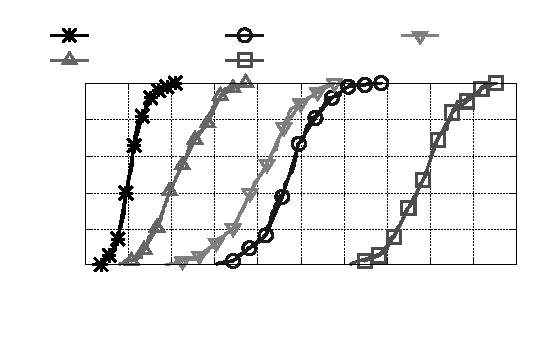
\includegraphics{dfnCDF}}%
    \gplfronttext
  \end{picture}%
\endgroup
}
    \caption{P4 and DFN}
    \label{fig:completion_time:openvswitch}
  \end{subfigure}
\caption{CDF of rule deployment times over 100 epochs.}
\label{fig:completion_time}
\end{figure}

SCC outperforms CU and COCONUT during rule deployment for two reasons.
First, SCC simply deploys rules to fewer switches, since it attempts
to minimize the number of switches to which it must do so.  Second,
SCC involves fewer phases of communication between the controller and
switches.  Here, COCONUT is worse than CU because it requires more
time to clean up old rules.  TSU is better than CU because CU needs to
update more switches.

\subsection{Memory Overhead in Switches}
\label{sec:eval:rules}

To evaluate the number of rules imposed on the switches by each
algorithm, we examined the per-switch logs of rule installations and
deletions over 100 consecutive path changes in the fat-tree topology
($\portsPerSwitch=8$).  We computed a time series of the total number
of rules installed across all switches in the network, if all 100 path
changes were included in one epoch.  This time series for each of SCC,
CU, and COCONUT is shown in \figref{fig:rule_number:fat_tree}.  We
repeated this evaluation on the DFN topology, but by breaking the
``busiest'' link; see \figref{fig:rule_number:dfn}.  Here, the
``busiest'' link is the link that causes the most path changes when
the link fails, which was 306 path changes in this case.  As these
figures show, SCC induced a rule overhead of significantly fewer rules
than CU and COCONUT, because SCC installs extra, send-back rules only
on selected switches on old paths.  In particular, SCC does not
temporarily retain old rules along with new rules, like CU and COCONUT
do.  Though TSU does not add extra rules on switches, old rules are
kept longer because TSU executes in multiple steps.


\begin{figure}[h]
\centering
  \begin{subfigure}[b]{0.49\linewidth}
    \resizebox{\linewidth}{!}{\footnotesize% GNUPLOT: LaTeX picture with Postscript
\begingroup
  \fontfamily{Times-Roman}%
  \selectfont
  \makeatletter
  \providecommand\color[2][]{%
    \GenericError{(gnuplot) \space\space\space\@spaces}{%
      Package color not loaded in conjunction with
      terminal option `colourtext'%
    }{See the gnuplot documentation for explanation.%
    }{Either use 'blacktext' in gnuplot or load the package
      color.sty in LaTeX.}%
    \renewcommand\color[2][]{}%
  }%
  \providecommand\includegraphics[2][]{%
    \GenericError{(gnuplot) \space\space\space\@spaces}{%
      Package graphicx or graphics not loaded%
    }{See the gnuplot documentation for explanation.%
    }{The gnuplot epslatex terminal needs graphicx.sty or graphics.sty.}%
    \renewcommand\includegraphics[2][]{}%
  }%
  \providecommand\rotatebox[2]{#2}%
  \@ifundefined{ifGPcolor}{%
    \newif\ifGPcolor
    \GPcolortrue
  }{}%
  \@ifundefined{ifGPblacktext}{%
    \newif\ifGPblacktext
    \GPblacktexttrue
  }{}%
  % define a \g@addto@macro without @ in the name:
  \let\gplgaddtomacro\g@addto@macro
  % define empty templates for all commands taking text:
  \gdef\gplbacktext{}%
  \gdef\gplfronttext{}%
  \makeatother
  \ifGPblacktext
    % no textcolor at all
    \def\colorrgb#1{}%
    \def\colorgray#1{}%
  \else
    % gray or color?
    \ifGPcolor
      \def\colorrgb#1{\color[rgb]{#1}}%
      \def\colorgray#1{\color[gray]{#1}}%
      \expandafter\def\csname LTw\endcsname{\color{white}}%
      \expandafter\def\csname LTb\endcsname{\color{black}}%
      \expandafter\def\csname LTa\endcsname{\color{black}}%
      \expandafter\def\csname LT0\endcsname{\color[rgb]{1,0,0}}%
      \expandafter\def\csname LT1\endcsname{\color[rgb]{0,1,0}}%
      \expandafter\def\csname LT2\endcsname{\color[rgb]{0,0,1}}%
      \expandafter\def\csname LT3\endcsname{\color[rgb]{1,0,1}}%
      \expandafter\def\csname LT4\endcsname{\color[rgb]{0,1,1}}%
      \expandafter\def\csname LT5\endcsname{\color[rgb]{1,1,0}}%
      \expandafter\def\csname LT6\endcsname{\color[rgb]{0,0,0}}%
      \expandafter\def\csname LT7\endcsname{\color[rgb]{1,0.3,0}}%
      \expandafter\def\csname LT8\endcsname{\color[rgb]{0.5,0.5,0.5}}%
    \else
      % gray
      \def\colorrgb#1{\color{black}}%
      \def\colorgray#1{\color[gray]{#1}}%
      \expandafter\def\csname LTw\endcsname{\color{white}}%
      \expandafter\def\csname LTb\endcsname{\color{black}}%
      \expandafter\def\csname LTa\endcsname{\color{black}}%
      \expandafter\def\csname LT0\endcsname{\color{black}}%
      \expandafter\def\csname LT1\endcsname{\color{black}}%
      \expandafter\def\csname LT2\endcsname{\color{black}}%
      \expandafter\def\csname LT3\endcsname{\color{black}}%
      \expandafter\def\csname LT4\endcsname{\color{black}}%
      \expandafter\def\csname LT5\endcsname{\color{black}}%
      \expandafter\def\csname LT6\endcsname{\color{black}}%
      \expandafter\def\csname LT7\endcsname{\color{black}}%
      \expandafter\def\csname LT8\endcsname{\color{black}}%
    \fi
  \fi
    \setlength{\unitlength}{0.0500bp}%
    \ifx\gptboxheight\undefined%
      \newlength{\gptboxheight}%
      \newlength{\gptboxwidth}%
      \newsavebox{\gptboxtext}%
    \fi%
    \setlength{\fboxrule}{0.5pt}%
    \setlength{\fboxsep}{1pt}%
\begin{picture}(4896.00,3024.00)%
    \gplgaddtomacro\gplbacktext{%
      \csname LTb\endcsname%%
      \put(860,640){\makebox(0,0)[r]{\strut{}$600$}}%
      \csname LTb\endcsname%%
      \put(860,997){\makebox(0,0)[r]{\strut{}$700$}}%
      \csname LTb\endcsname%%
      \put(860,1353){\makebox(0,0)[r]{\strut{}$800$}}%
      \csname LTb\endcsname%%
      \put(860,1710){\makebox(0,0)[r]{\strut{}$900$}}%
      \csname LTb\endcsname%%
      \put(860,2066){\makebox(0,0)[r]{\strut{}$1000$}}%
      \csname LTb\endcsname%%
      \put(860,2423){\makebox(0,0)[r]{\strut{}$1100$}}%
      \csname LTb\endcsname%%
      \put(980,440){\makebox(0,0){\strut{}$0$}}%
      \csname LTb\endcsname%%
      \put(1573,440){\makebox(0,0){\strut{}$0.2$}}%
      \csname LTb\endcsname%%
      \put(2165,440){\makebox(0,0){\strut{}$0.4$}}%
      \csname LTb\endcsname%%
      \put(2758,440){\makebox(0,0){\strut{}$0.6$}}%
      \csname LTb\endcsname%%
      \put(3350,440){\makebox(0,0){\strut{}$0.8$}}%
      \csname LTb\endcsname%%
      \put(3942,440){\makebox(0,0){\strut{}$1$}}%
      \csname LTb\endcsname%%
      \put(4535,440){\makebox(0,0){\strut{}$1.2$}}%
    }%
    \gplgaddtomacro\gplfronttext{%
      \csname LTb\endcsname%%
      \put(420,1531){\rotatebox{-270}{\makebox(0,0){\strut{}The total number of rules}}}%
      \put(2757,140){\makebox(0,0){\strut{}Time (s)}}%
      \csname LTb\endcsname%%
      \put(2157,2841){\makebox(0,0)[l]{\strut{}\sys}}%
      \csname LTb\endcsname%%
      \put(2157,2601){\makebox(0,0)[l]{\strut{}\cu}}%
      \csname LTb\endcsname%%
      \put(3420,2841){\makebox(0,0)[l]{\strut{}\tsu}}%
      \csname LTb\endcsname%%
      \put(3420,2601){\makebox(0,0)[l]{\strut{}\coconut}}%
    }%
    \gplbacktext
    \put(0,0){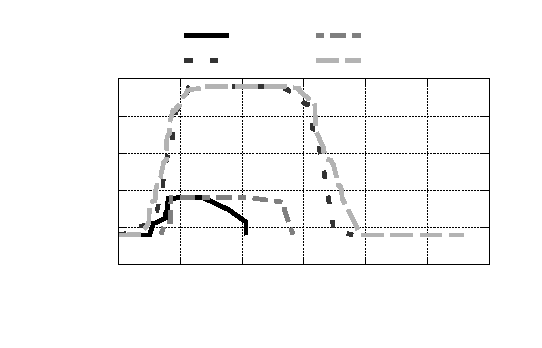
\includegraphics{rule}}%
    \gplfronttext
  \end{picture}%
\endgroup
}
    \caption{P4, fat-tree, 100 path changes}
    \label{fig:rule_number:fat_tree}
  \end{subfigure}
  \begin{subfigure}[b]{0.49\linewidth}
    \resizebox{\linewidth}{!}{\footnotesize% GNUPLOT: LaTeX picture with Postscript
\begingroup
  \fontfamily{Times-Roman}%
  \selectfont
  \makeatletter
  \providecommand\color[2][]{%
    \GenericError{(gnuplot) \space\space\space\@spaces}{%
      Package color not loaded in conjunction with
      terminal option `colourtext'%
    }{See the gnuplot documentation for explanation.%
    }{Either use 'blacktext' in gnuplot or load the package
      color.sty in LaTeX.}%
    \renewcommand\color[2][]{}%
  }%
  \providecommand\includegraphics[2][]{%
    \GenericError{(gnuplot) \space\space\space\@spaces}{%
      Package graphicx or graphics not loaded%
    }{See the gnuplot documentation for explanation.%
    }{The gnuplot epslatex terminal needs graphicx.sty or graphics.sty.}%
    \renewcommand\includegraphics[2][]{}%
  }%
  \providecommand\rotatebox[2]{#2}%
  \@ifundefined{ifGPcolor}{%
    \newif\ifGPcolor
    \GPcolortrue
  }{}%
  \@ifundefined{ifGPblacktext}{%
    \newif\ifGPblacktext
    \GPblacktexttrue
  }{}%
  % define a \g@addto@macro without @ in the name:
  \let\gplgaddtomacro\g@addto@macro
  % define empty templates for all commands taking text:
  \gdef\gplbacktext{}%
  \gdef\gplfronttext{}%
  \makeatother
  \ifGPblacktext
    % no textcolor at all
    \def\colorrgb#1{}%
    \def\colorgray#1{}%
  \else
    % gray or color?
    \ifGPcolor
      \def\colorrgb#1{\color[rgb]{#1}}%
      \def\colorgray#1{\color[gray]{#1}}%
      \expandafter\def\csname LTw\endcsname{\color{white}}%
      \expandafter\def\csname LTb\endcsname{\color{black}}%
      \expandafter\def\csname LTa\endcsname{\color{black}}%
      \expandafter\def\csname LT0\endcsname{\color[rgb]{1,0,0}}%
      \expandafter\def\csname LT1\endcsname{\color[rgb]{0,1,0}}%
      \expandafter\def\csname LT2\endcsname{\color[rgb]{0,0,1}}%
      \expandafter\def\csname LT3\endcsname{\color[rgb]{1,0,1}}%
      \expandafter\def\csname LT4\endcsname{\color[rgb]{0,1,1}}%
      \expandafter\def\csname LT5\endcsname{\color[rgb]{1,1,0}}%
      \expandafter\def\csname LT6\endcsname{\color[rgb]{0,0,0}}%
      \expandafter\def\csname LT7\endcsname{\color[rgb]{1,0.3,0}}%
      \expandafter\def\csname LT8\endcsname{\color[rgb]{0.5,0.5,0.5}}%
    \else
      % gray
      \def\colorrgb#1{\color{black}}%
      \def\colorgray#1{\color[gray]{#1}}%
      \expandafter\def\csname LTw\endcsname{\color{white}}%
      \expandafter\def\csname LTb\endcsname{\color{black}}%
      \expandafter\def\csname LTa\endcsname{\color{black}}%
      \expandafter\def\csname LT0\endcsname{\color{black}}%
      \expandafter\def\csname LT1\endcsname{\color{black}}%
      \expandafter\def\csname LT2\endcsname{\color{black}}%
      \expandafter\def\csname LT3\endcsname{\color{black}}%
      \expandafter\def\csname LT4\endcsname{\color{black}}%
      \expandafter\def\csname LT5\endcsname{\color{black}}%
      \expandafter\def\csname LT6\endcsname{\color{black}}%
      \expandafter\def\csname LT7\endcsname{\color{black}}%
      \expandafter\def\csname LT8\endcsname{\color{black}}%
    \fi
  \fi
    \setlength{\unitlength}{0.0500bp}%
    \ifx\gptboxheight\undefined%
      \newlength{\gptboxheight}%
      \newlength{\gptboxwidth}%
      \newsavebox{\gptboxtext}%
    \fi%
    \setlength{\fboxrule}{0.5pt}%
    \setlength{\fboxsep}{1pt}%
\begin{picture}(4896.00,3024.00)%
    \gplgaddtomacro\gplbacktext{%
      \csname LTb\endcsname%%
      \put(980,640){\makebox(0,0)[r]{\strut{}$13800$}}%
      \csname LTb\endcsname%%
      \put(980,937){\makebox(0,0)[r]{\strut{}$14100$}}%
      \csname LTb\endcsname%%
      \put(980,1234){\makebox(0,0)[r]{\strut{}$14400$}}%
      \csname LTb\endcsname%%
      \put(980,1532){\makebox(0,0)[r]{\strut{}$14700$}}%
      \csname LTb\endcsname%%
      \put(980,1829){\makebox(0,0)[r]{\strut{}$15000$}}%
      \csname LTb\endcsname%%
      \put(980,2126){\makebox(0,0)[r]{\strut{}$15300$}}%
      \csname LTb\endcsname%%
      \put(980,2423){\makebox(0,0)[r]{\strut{}$15600$}}%
      \csname LTb\endcsname%%
      \put(1100,440){\makebox(0,0){\strut{}$0$}}%
      \csname LTb\endcsname%%
      \put(1787,440){\makebox(0,0){\strut{}$0.5$}}%
      \csname LTb\endcsname%%
      \put(2474,440){\makebox(0,0){\strut{}$1$}}%
      \csname LTb\endcsname%%
      \put(3161,440){\makebox(0,0){\strut{}$1.5$}}%
      \csname LTb\endcsname%%
      \put(3848,440){\makebox(0,0){\strut{}$2$}}%
      \csname LTb\endcsname%%
      \put(4535,440){\makebox(0,0){\strut{}$2.5$}}%
    }%
    \gplgaddtomacro\gplfronttext{%
      \csname LTb\endcsname%%
      \put(420,1531){\rotatebox{-270}{\makebox(0,0){\strut{}The total number of rules}}}%
      \put(2817,140){\makebox(0,0){\strut{}Time (s)}}%
      \csname LTb\endcsname%%
      \put(2217,2841){\makebox(0,0)[l]{\strut{}\sys}}%
      \csname LTb\endcsname%%
      \put(2217,2601){\makebox(0,0)[l]{\strut{}\cu}}%
      \csname LTb\endcsname%%
      \put(3480,2841){\makebox(0,0)[l]{\strut{}\tsu}}%
      \csname LTb\endcsname%%
      \put(3480,2601){\makebox(0,0)[l]{\strut{}\coconut}}%
    }%
    \gplbacktext
    \put(0,0){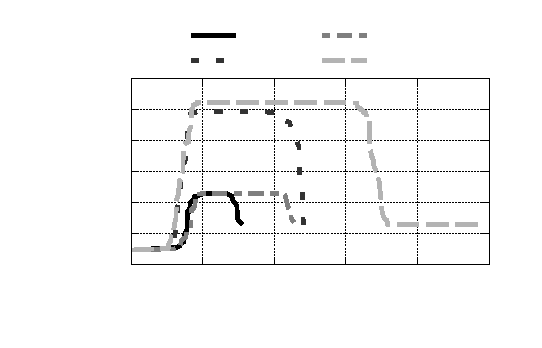
\includegraphics{isprule}}%
    \gplfronttext
  \end{picture}%
\endgroup
}
    \caption{P4, DFN, 306 path changes}
    \label{fig:rule_number:dfn}
  \end{subfigure}
\caption{Rules in the network during epoch installation.}
\label{fig:rule_number}
\end{figure}


\subsection{Rule Generation Time}
\label{sec:eval:rulegen}

Rule generation times for SCC are shown in \figref{fig:rulegen}.
There are two groups of box-plots shown in \figref{fig:rulegen}: one
for fat-tree topologies, and one for ISP topologies.  Of the listed
ISP topologies, the two numbers following each topology name (e.g.,
``40'' and ``61'' in ``Geant2012(40,61)'') are the number of switches
and links in the topology, respectively.  The numbers
in \figref{fig:rulegen} for the fat-tree topologies are
rule-generation times where the new epoch differs from the old epoch
by a sequence of 100 route changes present in the Facebook data (as
in \figref{fig:rule_number}).  The experiments with ISP topologies
reflect the cost of rule generation when a random link fails, causing
all routes traversing it to change.

\begin{figure}
\centering
  \resizebox{0.49\linewidth}{!}{% GNUPLOT: LaTeX picture with Postscript
\begingroup
  \fontfamily{Times-Roman}%
  \selectfont
  \makeatletter
  \providecommand\color[2][]{%
    \GenericError{(gnuplot) \space\space\space\@spaces}{%
      Package color not loaded in conjunction with
      terminal option `colourtext'%
    }{See the gnuplot documentation for explanation.%
    }{Either use 'blacktext' in gnuplot or load the package
      color.sty in LaTeX.}%
    \renewcommand\color[2][]{}%
  }%
  \providecommand\includegraphics[2][]{%
    \GenericError{(gnuplot) \space\space\space\@spaces}{%
      Package graphicx or graphics not loaded%
    }{See the gnuplot documentation for explanation.%
    }{The gnuplot epslatex terminal needs graphicx.sty or graphics.sty.}%
    \renewcommand\includegraphics[2][]{}%
  }%
  \providecommand\rotatebox[2]{#2}%
  \@ifundefined{ifGPcolor}{%
    \newif\ifGPcolor
    \GPcolortrue
  }{}%
  \@ifundefined{ifGPblacktext}{%
    \newif\ifGPblacktext
    \GPblacktexttrue
  }{}%
  % define a \g@addto@macro without @ in the name:
  \let\gplgaddtomacro\g@addto@macro
  % define empty templates for all commands taking text:
  \gdef\gplbacktext{}%
  \gdef\gplfronttext{}%
  \makeatother
  \ifGPblacktext
    % no textcolor at all
    \def\colorrgb#1{}%
    \def\colorgray#1{}%
  \else
    % gray or color?
    \ifGPcolor
      \def\colorrgb#1{\color[rgb]{#1}}%
      \def\colorgray#1{\color[gray]{#1}}%
      \expandafter\def\csname LTw\endcsname{\color{white}}%
      \expandafter\def\csname LTb\endcsname{\color{black}}%
      \expandafter\def\csname LTa\endcsname{\color{black}}%
      \expandafter\def\csname LT0\endcsname{\color[rgb]{1,0,0}}%
      \expandafter\def\csname LT1\endcsname{\color[rgb]{0,1,0}}%
      \expandafter\def\csname LT2\endcsname{\color[rgb]{0,0,1}}%
      \expandafter\def\csname LT3\endcsname{\color[rgb]{1,0,1}}%
      \expandafter\def\csname LT4\endcsname{\color[rgb]{0,1,1}}%
      \expandafter\def\csname LT5\endcsname{\color[rgb]{1,1,0}}%
      \expandafter\def\csname LT6\endcsname{\color[rgb]{0,0,0}}%
      \expandafter\def\csname LT7\endcsname{\color[rgb]{1,0.3,0}}%
      \expandafter\def\csname LT8\endcsname{\color[rgb]{0.5,0.5,0.5}}%
    \else
      % gray
      \def\colorrgb#1{\color{black}}%
      \def\colorgray#1{\color[gray]{#1}}%
      \expandafter\def\csname LTw\endcsname{\color{white}}%
      \expandafter\def\csname LTb\endcsname{\color{black}}%
      \expandafter\def\csname LTa\endcsname{\color{black}}%
      \expandafter\def\csname LT0\endcsname{\color{black}}%
      \expandafter\def\csname LT1\endcsname{\color{black}}%
      \expandafter\def\csname LT2\endcsname{\color{black}}%
      \expandafter\def\csname LT3\endcsname{\color{black}}%
      \expandafter\def\csname LT4\endcsname{\color{black}}%
      \expandafter\def\csname LT5\endcsname{\color{black}}%
      \expandafter\def\csname LT6\endcsname{\color{black}}%
      \expandafter\def\csname LT7\endcsname{\color{black}}%
      \expandafter\def\csname LT8\endcsname{\color{black}}%
    \fi
  \fi
    \setlength{\unitlength}{0.0500bp}%
    \ifx\gptboxheight\undefined%
      \newlength{\gptboxheight}%
      \newlength{\gptboxwidth}%
      \newsavebox{\gptboxtext}%
    \fi%
    \setlength{\fboxrule}{0.5pt}%
    \setlength{\fboxsep}{1pt}%
\begin{picture}(5760.00,3168.00)%
    \gplgaddtomacro\gplbacktext{%
      \csname LTb\endcsname%
      \put(484,1112){\makebox(0,0)[r]{\strut{}$0$}}%
      \csname LTb\endcsname%
      \put(484,1609){\makebox(0,0)[r]{\strut{}$1$}}%
      \csname LTb\endcsname%
      \put(484,2107){\makebox(0,0)[r]{\strut{}$2$}}%
      \csname LTb\endcsname%
      \put(484,2604){\makebox(0,0)[r]{\strut{}$3$}}%
      \csname LTb\endcsname%
      \put(484,3101){\makebox(0,0)[r]{\strut{}$4$}}%
      \csname LTb\endcsname%
      \put(1080,980){\rotatebox{25}{\makebox(0,0)[r]{\strut{}Abilene(11,14)}}}%
      \csname LTb\endcsname%
      \put(1682,980){\rotatebox{25}{\makebox(0,0)[r]{\strut{}Quest(20,31)}}}%
      \csname LTb\endcsname%
      \put(2284,980){\rotatebox{25}{\makebox(0,0)[r]{\strut{}Arnes(34,47)}}}%
      \csname LTb\endcsname%
      \put(2886,980){\rotatebox{25}{\makebox(0,0)[r]{\strut{}Geant2012(40,61)}}}%
      \csname LTb\endcsname%
      \put(3488,980){\rotatebox{25}{\makebox(0,0)[r]{\strut{}Dfn(58,87)}}}%
      \csname LTb\endcsname%
      \put(4692,980){\rotatebox{25}{\makebox(0,0)[r]{\strut{}FatTree(K=6)}}}%
      \csname LTb\endcsname%
      \put(5294,980){\rotatebox{25}{\makebox(0,0)[r]{\strut{}FatTree(K=8)}}}%
    }%
    \gplgaddtomacro\gplfronttext{%
      \csname LTb\endcsname%
      \put(176,2106){\rotatebox{-270}{\makebox(0,0){\strut{}Time (s)}}}%
    }%
    \gplgaddtomacro\gplbacktext{%
      \csname LTb\endcsname%
      \put(4081,1822){\makebox(0,0)[r]{\strut{}0.04}}%
      \put(4081,2297){\makebox(0,0)[r]{\strut{}0.06}}%
      \put(4081,2772){\makebox(0,0)[r]{\strut{}0.08}}%
    }%
    \gplgaddtomacro\gplfronttext{%
    }%
    \gplbacktext
    \put(0,0){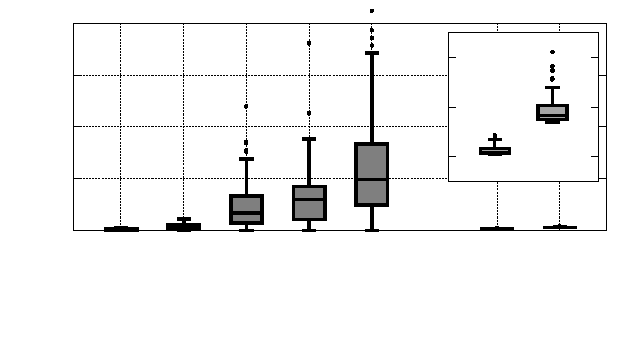
\includegraphics{boxperf}}%
    \gplfronttext
  \end{picture}%
\endgroup
}
  \caption{Distributions of SCC rule-generation times (100 path
  updates in fat-tree topologies; random link failure in ISP
  topologies).}
  \label{fig:rulegen}
\end{figure}


\figref{fig:rulegen} shows distributions of rule-generation times
as box-plots.  Each box shows the first, second (median),
and third quartiles, and whiskers extend to cover points that fall
within $1.5\times$ the interquartile range.  Outliers are shown as
dots.

Rule-generation times were minimal for the fat-tree topologies, even
for epochs modifying 100 routing paths.  Rule
generation times for ISP topologies were more substantial, but
typically completed in under $1\secs$ for all but one topology (DFN).
Rule generation for DFN rarely exceeded $3\secs$, but in these cases,
the link failure induced changes in over 250 routes.  While we
are encouraged by these results, there are numerous opportunities for
optimization in our current codebase (e.g., parallelization).

\subsection{Buffer Overhead}
\label{sec:eval:buffer}

\begin{figure}
\centering
  \resizebox{0.49\linewidth}{!}{% GNUPLOT: LaTeX picture with Postscript
\begingroup
  \fontfamily{Times-Roman}%
  \selectfont
  \makeatletter
  \providecommand\color[2][]{%
    \GenericError{(gnuplot) \space\space\space\@spaces}{%
      Package color not loaded in conjunction with
      terminal option `colourtext'%
    }{See the gnuplot documentation for explanation.%
    }{Either use 'blacktext' in gnuplot or load the package
      color.sty in LaTeX.}%
    \renewcommand\color[2][]{}%
  }%
  \providecommand\includegraphics[2][]{%
    \GenericError{(gnuplot) \space\space\space\@spaces}{%
      Package graphicx or graphics not loaded%
    }{See the gnuplot documentation for explanation.%
    }{The gnuplot epslatex terminal needs graphicx.sty or graphics.sty.}%
    \renewcommand\includegraphics[2][]{}%
  }%
  \providecommand\rotatebox[2]{#2}%
  \@ifundefined{ifGPcolor}{%
    \newif\ifGPcolor
    \GPcolortrue
  }{}%
  \@ifundefined{ifGPblacktext}{%
    \newif\ifGPblacktext
    \GPblacktexttrue
  }{}%
  % define a \g@addto@macro without @ in the name:
  \let\gplgaddtomacro\g@addto@macro
  % define empty templates for all commands taking text:
  \gdef\gplbacktext{}%
  \gdef\gplfronttext{}%
  \makeatother
  \ifGPblacktext
    % no textcolor at all
    \def\colorrgb#1{}%
    \def\colorgray#1{}%
  \else
    % gray or color?
    \ifGPcolor
      \def\colorrgb#1{\color[rgb]{#1}}%
      \def\colorgray#1{\color[gray]{#1}}%
      \expandafter\def\csname LTw\endcsname{\color{white}}%
      \expandafter\def\csname LTb\endcsname{\color{black}}%
      \expandafter\def\csname LTa\endcsname{\color{black}}%
      \expandafter\def\csname LT0\endcsname{\color[rgb]{1,0,0}}%
      \expandafter\def\csname LT1\endcsname{\color[rgb]{0,1,0}}%
      \expandafter\def\csname LT2\endcsname{\color[rgb]{0,0,1}}%
      \expandafter\def\csname LT3\endcsname{\color[rgb]{1,0,1}}%
      \expandafter\def\csname LT4\endcsname{\color[rgb]{0,1,1}}%
      \expandafter\def\csname LT5\endcsname{\color[rgb]{1,1,0}}%
      \expandafter\def\csname LT6\endcsname{\color[rgb]{0,0,0}}%
      \expandafter\def\csname LT7\endcsname{\color[rgb]{1,0.3,0}}%
      \expandafter\def\csname LT8\endcsname{\color[rgb]{0.5,0.5,0.5}}%
    \else
      % gray
      \def\colorrgb#1{\color{black}}%
      \def\colorgray#1{\color[gray]{#1}}%
      \expandafter\def\csname LTw\endcsname{\color{white}}%
      \expandafter\def\csname LTb\endcsname{\color{black}}%
      \expandafter\def\csname LTa\endcsname{\color{black}}%
      \expandafter\def\csname LT0\endcsname{\color{black}}%
      \expandafter\def\csname LT1\endcsname{\color{black}}%
      \expandafter\def\csname LT2\endcsname{\color{black}}%
      \expandafter\def\csname LT3\endcsname{\color{black}}%
      \expandafter\def\csname LT4\endcsname{\color{black}}%
      \expandafter\def\csname LT5\endcsname{\color{black}}%
      \expandafter\def\csname LT6\endcsname{\color{black}}%
      \expandafter\def\csname LT7\endcsname{\color{black}}%
      \expandafter\def\csname LT8\endcsname{\color{black}}%
    \fi
  \fi
    \setlength{\unitlength}{0.0500bp}%
    \ifx\gptboxheight\undefined%
      \newlength{\gptboxheight}%
      \newlength{\gptboxwidth}%
      \newsavebox{\gptboxtext}%
    \fi%
    \setlength{\fboxrule}{0.5pt}%
    \setlength{\fboxsep}{1pt}%
\begin{picture}(5760.00,3456.00)%
    \gplgaddtomacro\gplbacktext{%
      \csname LTb\endcsname%
      \put(682,707){\makebox(0,0)[r]{\strut{}$0$}}%
      \csname LTb\endcsname%
      \put(682,1378){\makebox(0,0)[r]{\strut{}$200$}}%
      \csname LTb\endcsname%
      \put(682,2048){\makebox(0,0)[r]{\strut{}$400$}}%
      \csname LTb\endcsname%
      \put(682,2719){\makebox(0,0)[r]{\strut{}$600$}}%
      \csname LTb\endcsname%
      \put(682,3389){\makebox(0,0)[r]{\strut{}$800$}}%
      \csname LTb\endcsname%
      \put(1555,575){\rotatebox{25}{\makebox(0,0)[r]{\strut{}600}}}%
      \csname LTb\endcsname%
      \put(2437,575){\rotatebox{25}{\makebox(0,0)[r]{\strut{}700}}}%
      \csname LTb\endcsname%
      \put(3319,575){\rotatebox{25}{\makebox(0,0)[r]{\strut{}800}}}%
      \csname LTb\endcsname%
      \put(4201,575){\rotatebox{25}{\makebox(0,0)[r]{\strut{}900}}}%
      \csname LTb\endcsname%
      \put(5083,575){\rotatebox{25}{\makebox(0,0)[r]{\strut{}1000}}}%
    }%
    \gplgaddtomacro\gplfronttext{%
      \csname LTb\endcsname%
      \put(176,2048){\rotatebox{-270}{\makebox(0,0){\strut{}Number of buffered packets}}}%
      \put(3372,154){\makebox(0,0){\strut{}Packets per second}}%
    }%
    \gplbacktext
    \put(0,0){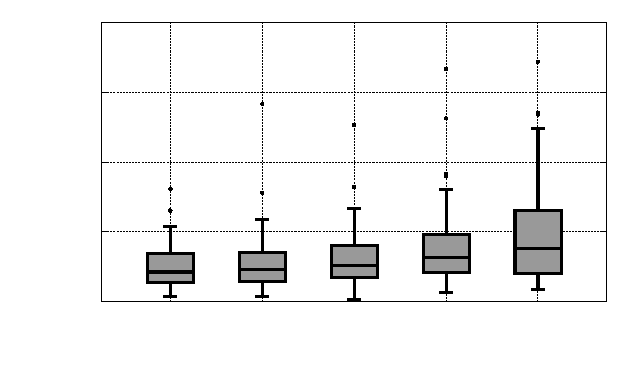
\includegraphics{buffer}}%
    \gplfronttext
  \end{picture}%
\endgroup
}
  \caption{Distributions of SCC maximum switch buffering during 10 path
  updates in fat-tree ($\portsPerSwitch = 8$).}
  \label{fig:buffer}
\end{figure}

In the tests reported in this section, we measured the peak number of
buffered packets on any switch, for different packet sending
rates. Each epoch in these tests involved ten path changes,
and \figref{fig:buffer} shows the distribution of the maximum number
of simultaneously buffered packets at any switch for 100 such epochs
for the fat-tree topology ($\portsPerSwitch = 8$).  As shown in the
figure, the number of buffered packets per switch rarely exceeded 200
and the buffering grew linearly as a function of packet sending rate.
Buffer sizes of commodity switches are usually in the $\megabytes$ or
even $\gigabytes$ range~\cite{buffer},
and so these buffering obligations should not be problematic.
